% ------------------------------------------------------------------------
% ------------------------------------------------------------------------
% ICMC: Modelo de Trabalho Acadêmico (tese de doutorado, dissertação de
% mestrado e trabalhos monográficos em geral) em conformidade com 
% ABNT NBR 14724:2011: Informação e documentação - Trabalhos acadêmicos -
% Apresentação
% ------------------------------------------------------------------------
% ------------------------------------------------------------------------

% Opções: 
%   Qualificação          = qualificacao 
%   Curso                 = doutorado/mestrado
%   Situação do trabalho  = pre-defesa/pos-defesa (exceto para qualificação)
%   Versão para impressão = impressao
\documentclass[qualificacao]{packages/icmc}

% ---------------------------------------------------------------------------
% Pacotes Opcionais
% ---------------------------------------------------------------------------
\usepackage{rotating}           % Usado para rotacionar o texto
\usepackage[all,knot,arc,import,poly]{xy}   % Pacote para desenhos gráficos
% Este pacote pode conflitar com outros pacotes gráficos como o ``pictex''
% Então é necessário usar apenas um dos pacotes conflitantes
\newcommand{\VerbL}{0.52\textwidth}
\newcommand{\LatL}{0.42\textwidth}
% ---------------------------------------------------------------------------

% [Falvojr] Pacotes adicionais
\usepackage{chronology}
\usepackage{rotating}

% [Falvojr] Comandos personalizados
% [Falvojr] https://tex.stackexchange.com/a/198372/54244
\newcommand\ytl[2]{
\parbox[b]{6em}{\hfill{\color{black} #1}~$\cdots\cdots$~}\makebox[0pt][c]{$\bullet$}\vrule\quad \parbox[c]{9cm}{\vspace{7pt}\color{black}\raggedright #2\\[7pt]}\\[-3pt]}
% [FalvoJr] Tipos de colunas personalizados
\newcolumntype{C}[1]{>{\centering\let\newline\\\arraybackslash\hspace{0pt}}m{#1}}
\newcolumntype{L}[1]{>{\raggedright\let\newline\\\arraybackslash\hspace{0pt}}m{#1}}

% ---
% Informações de dados para CAPA e FOLHA DE ROSTO
% ---
% Tanto na capa quanto nas folhas de rosto apenas a primeira letra da primeira palavra (ou nomes próprios) devem estar em letra maiúscula, todas as demais devem ser em letra minúscula.
\tituloPT{Uma Infraestrutura de Apoio ao Ensino e Aprendizagem de Línguas de Sinais}
\tituloEN{An Infrastructure to Support the Teaching and Learning of Sign Languages}
\autor[FalvoJr, V.]{Venilton Falvo Júnior}
\genero{M} % Gênero do autor (M = Masculino / F = Feminino)
\orientador[Orientadora]{Profa. Dra.}{Ellen Francine Barbosa}
%\coorientador{Prof. Dr.}{Fulano de Tal}
\curso{CCMC}
\data{01}{01}{2021} % Data do depósito
\idioma{PT} % Idioma principal do documento (PT = português / EN = inglês)
% ---


% ---
% RESUMOS
% ---

% Resumo em PORTUGUÊS
% conter no máximo 500 palavras
% conter no mínimo 1 e no máximo 5 palavras-chave
\textoresumo[brazil]{
    TODO
    }{línguas de sinais, educação, tecnologias da informação e comunicação}


% resumo em INGLÊS
% conter no máximo 500 palavras
% conter no mínimo 1 e no máximo 5 palavras-chave
\textoresumo[english]{
    TODO
    }{sign languages, education, information and communication technologies}


% ----------------------------------------------------------
% ELEMENTOS PRÉ-TEXTUAIS
% ----------------------------------------------------------

% Inserir a ficha catalográfica
\incluifichacatalografica{tex/pre-textual/ficha-catalografica.pdf}

% DEDICATÓRIA / AGRADECIMENTO / EPÍGRAFE
\textodedicatoria*{tex/pre-textual/dedicatoria}
\textoagradecimentos*{tex/pre-textual/agradecimentos}
\textoepigrafe*{tex/pre-textual/epigrafe}

% Inclui a lista de figuras
\incluilistadefiguras

% Inclui a lista de tabelas
\incluilistadetabelas

% Inclui a lista de quadros
\incluilistadequadros

% Inclui a lista de algoritmos
%\incluilistadealgoritmos

% Inclui a lista de códigos
%\incluilistadecodigos

% Inclui a lista de siglas e abreviaturas
%\incluilistadesiglas

% Inclui a lista de símbolos
%\incluilistadesimbolos

% ----
% Início do documento
% ----
\begin{document}
% ----------------------------------------------------------
% ELEMENTOS TEXTUAIS
% ----------------------------------------------------------
\textual

\chapter{Introdução}
\label{chapter:introducao}

\section{Contexto e Motivação}

%A maioria dos idiomas é baseada em sons audíveis. Sendo assim, as pessoas estão naturalmente acostumadas à língua falada e, para a maioria delas, a comunicação diária é regida pela audição \cite{Duke2009}. No entanto, existem 466 milhões de pessoas, cerca de 6,1\% da população mundial, com perda auditiva incapacitante \cite{WHO2018}. Com isso, grande parte delas têm a necessidade de ``ouvir com os olhos'', algo possível por meio das línguas de sinais.

%As línguas de sinais são formas de comunicação essencialmente baseadas no sentido da visão. Assim, conversas e informações são transmitidas visualmente usando diferentes formas/movimentos das mãos. Para isso, seus usuários combinam movimentos articulados das mãos, expressões faciais, movimentos da cabeça e do corpo para comunicar sentimentos, intenções, humor, além de ideias complexas ou abstratas \cite{Duke2009}.

Segundo a Organização Mundial de Saúde (OMS), existem 466 milhões de pessoas, cerca de 6,1\% da população mundial, com perda auditiva incapacitante \cite{OMS2018}. Sendo assim, grande parte delas têm a necessidade de ``ouvir com os olhos'', algo possível por meio das línguas de sinais, as quais permitem que conversas e informações sejam transmitidas visualmente usando diferentes formas de comunicação sinalizadas. Para isso, seus usuários combinam movimentos articulados das mãos, expressões faciais e movimentos corporais para se comunicarem \cite{Duke2009}.

De acordo com a Organização das Nações Unidas (ONU), tecnicamente não existe uma língua de sinais universal, principalmente devido às singularidades linguísticas em questão, as quais impõem barreiras contundentes para a universalidade das línguas de sinais \cite{ONU2019, Quadros2019}. Nesse contexto, a Federação Mundial de Surdos (WFD -- \textit{World Federation of the Deaf}) estima que existam aproximadamente 72 milhões de surdos em todo o mundo, os quais coletivamente utilizam mais de 300 línguas de sinais diferentes \cite{ONU2019}.

Um relatório da WFD relata que tamanha diversidade agrava ainda mais a falta de consistência em todo o mundo nos processos de interpretação e tradução das línguas de sinais, evidenciando uma linha de pesquisa relevante \cite{Napier2019}. De acordo com \citeonline{Duke2009}, caso todas as línguas de sinais fossem unificadas, elas representariam o terceiro idioma mais usado nos Estados Unidos e o quarto idioma mais usado no mundo.

No Brasil, a Língua Brasileira de Sinais (Libras) foi reconhecida oficialmente em 2002 \cite{Honora2017,Quadros2019}. Desde então, algumas iniciativas foram fomentadas em âmbito nacional para inclusão social/cultural de seus usuários. Segundo o último censo demográfico do Instituto Brasileiro de Geografia e Estatística (IBGE) \cite{IBGE2010}, existem cerca de 9,7 milhões de pessoas com limitações auditivas no Brasil, o que equivale à 5,1\% da população. Vale ressaltar que esses dados estatísticos não foram coletados visando um levantamento sobre o cenário nacional com relação à Libras. Todavia, tais pessoas são usuárias em potencial dessa língua de sinais, mas infelizmente apenas uma parcela delas terá acesso à alfabetização, tendo em vista as dificuldades socioeconômicas do país.

Por outro lado, o advento da tecnologia vem impactando significativamente o processo de ensino e aprendizagem das línguas de sinais. Com isso, soluções disruptivas, como o uso de óculos de realidade aumentada ou técnicas de tradução simultânea, podem orientar o desenvolvimento de aplicações educacionais cada vez mais efetivas e acessíveis aos aprendizes das línguas de sinais \cite{Napier2019}.

Em uma perspectiva relacionada, as Tecnologias de Informação e Comunicação (TICs) têm alterado não apenas as interações pessoais, mas também as práticas de ensino. A globalização das TICs criou um contexto educacional sem precedentes: mais flexível, conectado e inteligente. As tecnologias portáteis, juntamente com as redes de computadores, tornam-se cada vez mais presentes na vida cotidiana, promovendo um acesso onipresente à informação \cite{Cilli2017}.

As TICs dizem respeito a processos e produtos que estão em constante transformação, provindos especialmente da eletrônica, da microeletrônica e da área de telecomunicações. O escopo de ação dessas tecnologias é virtual e utiliza a informação como o principal insumo \cite{Cilli2017}. Sendo assim, diferentes áreas de conhecimento tendem a se beneficiar com o uso dessas tecnologias, principalmente em domínios complexos como o da educação inclusiva baseada em línguas de sinais.

Em sentido amplo, educação indica o meio em que os hábitos, costumes e valores de uma determinada sociedade/grupo são transferidos de uma geração para outra, e estes vão se formando a partir de situações presenciadas e de experiências adquiridas no decorrer da vida. Em específico, educação é um processo contínuo de desenvolvimento das faculdades físicas, intelectuais e morais do ser humano para que este se integre da melhor forma possível em sua comunidade \cite{Cilli2017,Quadros2019}. Note que, em ambas as perspectivas, a inclusão social é essencial para que o indivíduo tenha acesso adequado à educação e isso independe de sua língua dominante (de sinais ou falada) \cite{Quadros2019}. 

A educação é um processo continuo de desenvolvimento para que a pessoa se integre à sociedade ou grupo ao qual pertence \cite{Cilli2017,Quadros2019}. Logo, a inclusão social e digital são aspectos importantes no processo educacional moderno. Nessa perspectiva, as TICs podem contribuir para tornar as práticas educacionais mais inclusivas, personalizando o processo de ensino e aprendizagem ao contexto dos alunos, especialmente em cenários onde a diversidade linguística é essencial, como na educação bilíngue.

\section{Objetivos}

Tendo em vista o contexto e motivações apresentados, este projeto tem como principal objetivo prover uma infraestrutura, que orquestre recursos educacionais visando a educação inclusiva de surdos. Ressalta-se que o conceito de inclusão, na identidade surda, traz consigo um ideal baseado na educação bilíngue. Sendo assim, a infraestrutura em questão permitirá o desenvolvimento de aplicações educacionais bilíngues. %Em especial, a arquitetura SOA foi escolhida devido a sua flexibilidade e compatibilidade com estilos arquiteturais já consolidados na Engenharia de Software (ES) e Industria. %Como por exemplo, \textbf{Re}presentational \textbf{S}tate \textbf{T}ransfer (REST) \cite{Fielding2000} ou Microserviços \cite{Sommerville2015}, os quais, inclusive, podem ser implementados juntos.
Com base nesse objetivo geral, são estabelecidos os seguintes objetivos específicos:

\begin{enumerate}
\item Identificação de um conjunto básico de especificações técnicas e requisitos de desenvolvimento relacionados à educação inclusiva por meio das línguas de sinais, com o apoio das TICs; %Obtido, principalmente, através de um Mapeamento Sistemático (MS);
\item Proposição de uma arquitetura que favoreça o desenvolvimento de soluções educacionais inclusivas no contexto das línguas de sinais. Desta forma, a infraestrutura resultante proverá todos os insumos necessários para o desenvolvimento de ferramentas de Tecnologia Assistiva (TA), as quais devem potencializar de forma significativa a participação do surdo no desempenho de suas tarefas educacionais.
\item Avaliação da arquitetura proposta por especialistas, tendo em vista o refinamento/evolução da abordagem em função de feedbacks das áreas da ES, educação e línguas de sinais. Com isso, a arquitetura é devidamente instanciada e implantada, provendo uma infraestrutura de apoio à criação de soluções educacionais com suporte a línguas de sinais;
\item Desenvolvimento de uma aplicação educacional móvel, criada a partir da infraestrutura proposta, no contexto da educação bilíngue (Libras e Português). Para isso, um tópico educacional específico será definido tendo em vista o ensino e aprendizagem por meio das línguas em questão. %Nesse caso, a Matemática foi o tópico educacional escolhido por ser uma disciplina neutra, ou seja, que não favorece nenhuma das línguas (falada ou de sinais). 
Além disso, é importante ressaltar que as soluções geradas a partir dessa arquitetura/infraestrutura comum serão sensíveis ao contexto de seus usuários, obtendo informações importantes para o tratamento de eventuais regionalidades (presentes em ambas as línguas, falada e de sinais);
\item Condução de experimentos com aprendizes e tutores, %preferencialmente em uma sala de aula inclusiva, 
a fim de avaliar a TA criada e, indiretamente, sua respectiva arquitetura.
\end{enumerate}

Os objetivos apresentados buscam responder à seguinte questão de pesquisa: Como as TICs, aliadas a boas práticas de desenvolvimento e infraestrutura, podem auxiliar/facilitar a criação de aplicações educacionais inclusivas para surdos, por meio de uma interface pública e bilíngue?

%Para o desenvolvimento de ambientes educacionais efetivos, é essencial que sejam consideradas as características intrínsecas dos aprendizes, incluindo suas limitações físicas. Entretanto, usuários com deficiência auditiva ainda enfrentam dificuldades no processo de ensino devido a ambientes inadequados de aprendizagem, que geralmente não foram planejados/projetados pensando em usuários de línguas de sinais \cite{Snoddon2018}.

%Uma era disruptiva é evidente, na qual a disseminação de novas tecnologias e a interconectividade global têm potencial para acelerar o progresso humano, diminuir a barreira digital e desenvolver soluções cada vez mais inclusivas \cite{Itu2019a,Itu2019b}. Por esses motivos, é necessário refletir sobre o ensino e aprendizagem das línguas de sinais, considerando o crescente uso de tecnologias no campo educacional.

%De fato, as TICs podem facilitar o acesso ao conhecimento, especialmente no contexto de pessoas com algum tipo de deficiência. Nesse cenário, este trabalho apresenta a condução de um Mapeamento Sistemático (MS), a fim de destacar o estado da arte considerando o uso de tecnologias no ensino e aprendizagem de línguas de sinais.

%O MS selecionou 139 estudos primários através de uma abordagem de busca baseada em \textit{Quasi-Gold Standard} (QGS) \cite{Zhang2011}, obtendo uma visão geral sobre as principais soluções de software, hardware e contribuições teóricas relacionadas ao domínio em questão. Dessa forma, foi possível delinear os estudos selecionados com foco na Libras. Considerando o cenário nacional, a Libras está presente em 16 destes trabalhos, sendo superada apenas pela \textit{American Sign Language} (ASL), e representando cerca de 11,5\% dos estudos primários do MS. De forma complementar, outros 46 estudos, selecionados manualmente em eventos nacionais, foram incorporados aos estudos primários com a intenção de expandir os resultados e discussões no âmbito da Libras.

\section{Organização}

Neste capítulo foi apresentado o contexto geral ao qual este trabalho de doutorado está inserido, além das motivações e justificativas para o seu desenvolvimento e os objetivos almejados para sua conclusão. 

O Capítulo \ref{chapter:fundamentacao-teorica} apresenta a fundamentação teórica que embasa este trabalho, abordando duas temáticas principais: línguas de sinais e TICs, com ênfase na educação inclusiva e tecnologia assistiva, respectivamente.

O Capítulo \ref{chapter:mapeamento-sistematico} apresenta um mapeamento sistemático sobre o cenário atual de pesquisas envolvendo o ensino e aprendizagem com línguas de sinais por meio do uso de tecnologias. Desta forma, foi possível analisar os cenários global e nacional no que tange o escopo de pesquisa em questão.

O Capítulo \ref{chapter:proposta} apresenta a proposta deste trabalho de doutorado, retomando a caracterização da pesquisa e apresentando as atividades previstas, cronograma, procedimentos metodológicos, resultados esperados e publicações. 
\chapter{Fundamentação Teórica}
\label{chapter:fundamentacao-teorica}

\section{Considerações Iniciais}
\label{fundamentacao-teorica:inicio}

Neste capítulo é apresentado um levantamento bibliográfico sobre os principais conceitos teóricos que fundamentam este projeto. Na Seção \ref{fundamentacao-teorica:linguas-sinais}, o conceito de línguas de sinais é explanado, com ênfase na caracterização do tema tendo em vista o contexto educacional, bem como os principais desafios e problemas identificados. A Seção \ref{fundamentacao-teorica:tic} fundamenta o conceito das TICs, apresentando suas principais ferramentas de apoio ao ensino e aprendizagem, as quais têm grande potencial no apoio à educação inclusiva.

\section{Línguas de Sinais}
\label{fundamentacao-teorica:linguas-sinais}

Segundo \citeonline{Honora2017}, as línguas de sinais são naturais, pois surgiram espontaneamente do convívio entre as pessoas. Elas podem ser comparadas à complexidade e à expressividade das línguas faladas, já que podem transmitir qualquer conceito, concreto ou abstrato, emocional ou racional, complexo ou simples. Tratam-se de línguas organizadas e não de simples junções de gestos, o que as caracterizariam apenas como linguagens. Sendo assim, por terem regras e serem totalmente estruturadas, são denominadas línguas.

Entretanto, tal classificação precisou de algum tempo e, principalmente, pesquisa para ser aceita formalmente. Segundo \citeonline{Quadros2019}, os estudos das línguas de sinais, inicialmente tiveram como função convencer os linguistas e demais agentes de políticas linguísticas/educacionais de que elas eram, de fato, línguas. Havia uma compreensão equivocada, com base no senso comum, de que as línguas de sinais seriam universais por usarem o corpo em movimentos supostamente compreendidos como gestos. Os gestos, nesse caso, eram associados à ideia de que a produção das línguas de sinais representaria formas universais e de que elas seriam facilmente entendidas por qualquer pessoa. Desse modo, haveria apenas uma única ``linguagem'' de sinais, reduzindo o status de língua para apenas uma forma de comunicação gestual compartilhável \cite{Quadros2004}. No entanto, o reconhecimento dos níveis linguísticos nas línguas de sinais permite seu enquadramento, no campo da Linguística, tanto do ponto de vista teórico, quanto aplicado \cite{Quadros2019}.

Para \citeonline{Gesser2009}, essa suposta universalidade é uma das crenças mais recorrentes quando se fala em língua de sinais. Nessa conjuntura, embora se possa traçar um histórico das origens e apontar possíveis parentescos e semelhanças no nível estrutural das línguas humanas (sejam elas faladas ou de sinais), alguns fatores favorecem a diversificação e a mudança da língua dentro de uma comunidade linguística, como, por exemplo, a extensão e a descontinuidade territorial, além da diversidade cultural oriunda desses acontecimentos.

Além disso, \citeonline{Gesser2009} afirma que, o que pode ser considerado universal é o impulso dos indivíduos para a comunicação e, no caso dos usuários das línguas de sinais, esse impulso é sinalizado. Sendo assim, considerar a ideia de universalidade, traz implicitamente uma tendência de simplificar a riqueza linguística em questão, sugerindo que talvez para os surdos fosse mais fácil se todos usassem uma língua única/uniforme. Nesse sentido, tendo em vista que as línguas de sinais são naturais, seria improvável obter tal uniformidade. De forma complementar, essa ideia tende a ser mais plausível em línguas artificiais, mas essas não se encaixam ao contexto proposto neste trabalho.
%Mesmo que, do ponto de vista prático, tal uniformidade fosse desejável, seria improvável a existência de uma língua que, além de única, permanecesse imutável em cinco continentes.

De acordo com \citeonline{Honora2017}, as línguas de sinais distinguem-se das línguas faladas porque se utilizam do meio visual-espacial em detrimento do oral-auditivo, ou seja, na elaboração das línguas de sinais é necessário olhar os movimentos que o emissor realiza para entender sua mensagem. Já na língua falada é preciso apenas ouvi-la, sem necessariamente estar olhando para o emissor. Um exemplo é um casal de ouvintes que conversa mesmo quando estão em cômodos separados em uma casa. Por outro lado, nas línguas de sinais esta situação é impossível, pois é necessário estar ao alcance da visão para que o sinal seja notado e interpretado pelos receptores.

\citeonline{Honora2017} e \citeonline{Quadros2019} ressaltam que as línguas de sinais são vivas, pois estão em constante transformação com o surgimento de novos sinais, sendo introduzidos pela comunidade surda de acordo com a sua necessidade. Conforme apresentado anteriormente, as línguas de sinais não são universais. Portanto, cada uma tem a sua própria estrutura gramatical e, assim como não temos uma língua falada única, também não temos uma língua de sinais universal. Além disso, mesmo países com a mesma língua falada podem possuir línguas de sinais diferentes. Um exemplo é o caso de Brasil e Portugal, países que compartilham a língua portuguesa, mas têm línguas de sinais diferentes. O contrário acontece com os Estados Unidos e o Canadá, que possuem a mesma língua falada e de sinais.

Nesse contexto, \citeonline{Quadros2019} descreve que estudos das diferentes línguas de sinais do mundo evidenciaram as especificidades dos sinais de cada país, identificando inclusive sua autonomia diante das línguas nacionalmente faladas. Essa autonomia é evidenciada também pelo fato de as línguas de sinais pertencerem a diferentes famílias linguísticas, de origens distintas das línguas faladas em seus respectivos países. Por exemplo, a Libras tem origem na LSF (Língua de Sinais Francesa), enquanto a LGP (Língua Gestual Portuguesa) tem origem na STS (Língua de Sinais Sueca). Considerando essas origens, apesar de a língua falada ser a portuguesa no Brasil e em Portugal (exceto pelas variações já estabelecidas), a Libras e a LGP são completamente diferentes, pois cada uma apresenta um conjunto de fonemas próprios, que tornam as palavras muito distintas, para não falar das diversas estruturas existentes em uma língua e noutra.

Até então, esta seção apresentou algumas das principais características das línguas de sinais: (i) são línguas e não linguagens, pois possuem uma estrutura e regras próprias; (ii) não são universais, porque surgiram naturalmente, diante da necessidade de comunicação entre grupos geograficamente e culturalmente distintos; (iii) uniformidade na língua falada não garante o mesmo com relação às línguas de sinais, à exemplo de Brasil e Portugal.

Em tempo, vale ressaltar que as temáticas apresentadas possuem uma série de terminologias que advém de diferentes áreas do conhecimento, fato que muitas vezes pode dar margem para interpretações equivocadas. Nessa perspectiva, \citeonline{Quadros2019} apresenta um glossário com um conjunto de definições especificamente selecionados para o esclarecimento de conceitos relevantes no domínio das línguas de sinais. O glossário em questão foi adaptado, com ênfase em termos pertinentes a esta pesquisa, os quais são apresentados em formato de Tabelas no decorrer desta seção. Nesse sentido, as Tabelas \ref{tab:glossario:tipos-linguas}, \ref{tab:glossario:modalidades-linguas}, \ref{tab:glossario:representacoes-visual-espaciais} e \ref{tab:glossario:termos-usuarios} organizam tais definições, destacando-as de acordo com sua importância.

\begin{table}[htbp]
\caption{Glossário: tipos de línguas}
\label{tab:glossario:tipos-linguas}
\begin{tabularx}{\textwidth}{l|X} \hline
\textbf{Língua de sinais} & \textbf{O termo ``língua de sinais'' se refere às línguas que usam a modalidade visual-espacial. Esse termo é usado genericamente em alusão a qualquer língua de sinais específica.} \\ \hline
Língua falada & As línguas faladas são as línguas orais-auditivas, ou seja, as línguas que utilizam os canais oral (aparelho vocal) e auditivo (aparelho auditivo) para produzir e perceber a fala. Essa forma será usada neste trabalho para se opor as línguas de sinais. O termo ``língua falada'' é pre ferido ao termo ``língua oral'' porque as línguas de sinais também são línguas orais, no sentido de serem produzidas ``oralmente'' em oposição à forma escrita. \\ \hline
\end{tabularx}
\caption*{Fonte: \citeonline{Quadros2019}.}
\end{table}

\begin{table}[htbp]
\caption{Glossário: modalidades de línguas}
\label{tab:glossario:modalidades-linguas}
\begin{tabularx}{\textwidth}{l|X} \hline
Oral-auditiva & A língua oral-auditiva se refere às línguas faladas. O português, por exemplo, é uma língua oral-auditiva, produzida oralmente com a intenção de ser ouvida. \\ \hline
\textbf{Visual-espacial} & \textbf{As línguas de sinais são visual-espaciais, pois são articuladas no espaço por meio do corpo (mãos, face etc) e acessadas visualmente, ou seja, pela visão. Os sinais são produzidos corporalmente e vistos uns pelos outros (não utilizam sons e não são ouvidos). De forma análoga a visual-espaciais, a nomenclatura gestual-espaciais também é aceita.} \\ \hline
\end{tabularx}
\caption*{Fonte: \citeonline{Quadros2019}.}
\end{table}

Em especial, a \autoref{tab:glossario:representacoes-visual-espaciais}, define formalmente os termos ``gestos'' e ``sinais''. De forma resumida, um gesto pode representar a origem de um sinal, se tornando linguístico e evoluindo sua respectiva língua de sinais. Por outro lado, ainda existem pesquisas visando a desambiguação desses termos, as quais podem culminar na gramaticalização dos gestos nas línguas de sinais. Por outro lado, a \autoref{tab:glossario:termos-usuarios} apresenta os principais termos atribuídos aos usuários das línguas de sinais. Nesse contexto, \citeonline{Quadros2019} afirma que o termo ``surdo'' é o mais apropriado considerando os usuários das línguas de sinais, pois não carrega consigo estereótipos médicos (``deficiente auditivo'') e/ou relacionados a impossibilidade de fala (``surdo-mudo'').

Um adendo importante, ainda considerando a \autoref{tab:glossario:termos-usuarios}, é de que existem outros termos comumente atribuídos aos usuários das línguas de sinais. Neste cenário, mas em uma perspectiva mais ampla, \citeonline{Oliveira2016} apresenta que ao longo dos anos diversos termos foram considerados apropriados para representar as pessoas com algum tipo de deficiência física. Entretanto, o termo recomendado atualmente é ``Pessoa com Deficiência'' (PcD), pois ele indica que há algum tipo de deficiência sem que isso inferiorize o indivíduo. Sendo assim, o termo ``PcD'' será utilizado neste trabalho em contextos mais genéricos, onde a terminologia ``surdo'' não seja adequada.

\begin{table}[htbp]
\caption{Glossário: representações visual-espaciais}
\label{tab:glossario:representacoes-visual-espaciais}
\begin{tabularx}{\textwidth}{l|X} \hline
\textbf{Gestos} & \textbf{A Gestos representam produções a partir do corpo para se referir a diferentes níveis de comportamento com ou sem significado . Os gestos são usados tanto nas línguas faladas quanto nas línguas de sinais. Nas línguas faladas, como os gestos são produzidos pelo corpo, são facilmente identificados como gestos. No caso das línguas de sinais, os gestos se apresentam na mesma modalidade dos sinais. Assim, nem sempre é fácil identificar os gestos e os sinais como produções que apresentem fronteiras claras. Os gestos podem se fundir com os sinais e se tornarem linguísticos. Os gestos nas línguas faladas são identificados como extralinguísticos. No entanto, os estudos com as línguas de sinais têm apontado para a gramaticalização dos gestos nas línguas de sinais. Talvez os gestos também possam ser considerados elementos linguísticos nas línguas faladas.} \\ \hline
\textbf{Sinais} & \textbf{As pessoas que usam uma língua de sinais normalmente se referem as palavras que a compõem como ``sinais''. Nesse caso , os ``sinais'' correspondem às ``palavras'' de sua língua falada.} \\ \hline
\end{tabularx}
\caption*{Fonte: \citeonline{Quadros2019}.}
\end{table}

\begin{table}[htbp]
\caption{Glossário: termos comuns atribuídos a usuários de línguas de sinais}
\label{tab:glossario:termos-usuarios}
\begin{tabularx}{\textwidth}{l|X} \hline
Deficiente auditivo & Deficiente auditivo é um termo para se referir aos surdos a partir da perspectiva médica. Os surdos que integram comunidades surdas e usam uma língua de sinais normalmente não utilizam o termo deficiente auditivo, pois preferem ser chamados de surdos. Por outro lado, a expressão deficiente auditivo é utilizada por surdos que não aprendem a língua de sinais. São surdos submetidos à oralização com exclusão da língua de sinais. \\ \hline
\textbf{Surdo} & \textbf{É como se identifica a pessoa que é surda, identificação considerada a mais apropriada entre os surdos que usam a língua de sinais.} \\ \hline
Surdo-mudo & É uma forma antiga de se referir aos surdos. Atualmente, os surdos consideram essa forma politicamente incorreta, pois a expressão ``mudo'' indica impossibilidade de falar, o que não expressa, de fato, a identidade surda. Os surdos podem falar e usam uma língua de sinais para se expressarem. \\ \hline
\end{tabularx}
\caption*{Fonte: \citeonline{Quadros2019}.}
\end{table}

Com isso, temas relacionados ao domínio em questão podem ser explorados de forma adequada, tendo em vista a definição e esclarecimento das principais terminologias usadas no campo das línguas de sinais, especialmente no contexto deste trabalho. Considerando as subseções a seguir, primeiramente a Libras é apresentada em detalhes, com suas respectivas características e políticas públicas voltadas para a inclusão social. Em seguida, a educação inclusiva é abordada, com ênfase no letramento bilíngue. Por fim, alguns dos desafios e problemas identificados no contexto das línguas de sinais são discutidos.

\subsection{Libras}
\label{fundamentacao-teorica:linguas-sinais:libras}

No Brasil a história das línguas de sinais teve início em 1857, com a chegada do educador francês Hernest Huet, um ex-aluno surdo do Instituto de Paris, que trouxe consigo o conhecimento sobre o alfabeto manual francês e a LSF, tidas como as principais influências para a criação da Libras \cite{Honora2017,Almeida2015}. Por sua vez, Libras é a sigla para \textbf{Lí}ngua \textbf{Bra}sileira de \textbf{S}inais, cuja comunicação é realizada através de gestos, expressões faciais e corporais, características em consonância com a modalidade visual-espacial.

Nesse contexto, muitas pessoas acreditam que a Libras é um alfabeto manual, algo equivocado tendo em vista as discussões supracitadas sobre a completude linguística das línguas de sinais. De acordo com \citeonline{Gesser2009}, essa inverdade fixa-se na falácia de que as línguas de sinais são limitadas e que a única forma de expressão comunicativa seria uma adaptação das letras realizadas manualmente, convencionadas e representadas a partir da língua oral.

Segundo \citeonline{Gesser2009}, o alfabeto manual, utilizado para soletrar manualmente as palavras (também referido como datilologia), é apenas um recurso utilizado por falantes da língua de sinais. Não é uma língua, mas sim um código de representação das letras alfabéticas. Sendo assim, tem uma função relevante na interação entre os usuários da línguas de sinais, principalmente para soletrar nomes próprios (pessoas ou lugares), siglas e algum vocábulo inexistente na língua de sinais.

No Brasil, o alfabeto manual é composto de 27 sinais, contando o grafema ç que é a configuração de mão da letra c com movimento trêmulo \cite{Gesser2009}. Cada formato da mão corresponde a uma letra do alfabeto do português brasileiro (\autoref{fig:libras-alfabeto}). De forma análoga também temos os números (\autoref{fig:libras-numeros}), os quais servem de referência para uma série de outros sinais, como por exemplo os dias da semana (\autoref{fig:libras-dias-semana}).

\begin{figure}[htbp]
\caption{Libras: alfabeto manual.}
\label{fig:libras-alfabeto}
\centerline{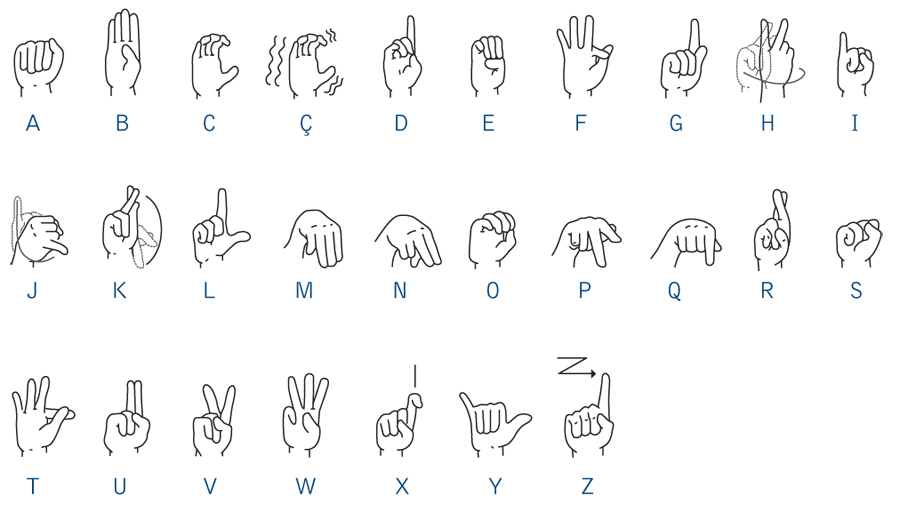
\includegraphics[width=0.95\textwidth]{images/libras-alfabeto.jpg}}
\caption*{Fonte: Centro de Educação para Surdos Rio Branco \url{www.ces.org.br}.}
\end{figure}

De modo complementar, tendo em mente a plenitude linguística da Libras, existem unidades mínimas para a formação dos sinais, tais como os fonemas nas línguas faladas. Considerando as características estruturais da Libras, seus sinais podem ser decompostos em cinco parâmetros \cite{Honora2017, Quadros2019}:

\begin{itemize}
    \item \textbf{Configuração das Mãos (CM)}: tem relação com as formas das mãos para a execução do sinal. Pode ser representado por uma letra do alfabeto, número ou outras formas de colocar a mão no momento inicial do sinal. A configuração das mãos é a representação de como estará a mão dominante (direita para os destros e esquerda para os canhotos) no momento inicial do sinal. Alguns sinais também poder ser representados pelas duas mãos;
    \item \textbf{Localização (L)}: também chamado de Ponto de Articulação (PA), diz respeito ao local onde incide a mão configurada para a execução do sinal. Pode ser alguma parte do corpo ou o sinal poderá ser realizado num espaço neutro vertical (ao lado do corpo) ou espaço neutro horizontal (na frente do corpo);
    \item \textbf{Movimento (M)}: alguns sinais têm movimento, outros não, são sinais estáticos. Movimento é o deslocamento da mão no espaço para execução do sinal;
    \item \textbf{Orientação ou Direcionalidade (O/D)}: é a direção que o sinal terá para ser executado;
    \item \textbf{Expressão Facial e/ou Corporal (EF/EC)}: muitos sinais necessitam de um complemento facial e até corporal para fazer com que sejam compreendidos. A expressão facial são as feições feitas pelo rosto para dar vida e entendimento ao sinal executado.
\end{itemize}

\begin{figure}[htbp]
\caption{Libras: números.}
\label{fig:libras-numeros}
\centerline{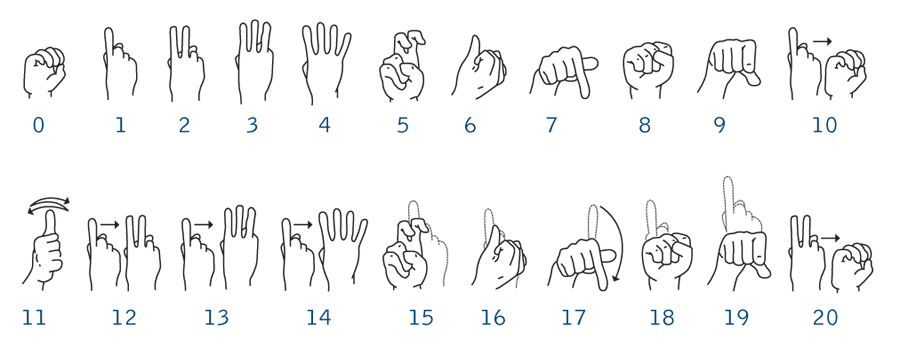
\includegraphics[width=0.95\textwidth]{images/libras-numeros.jpg}}
\caption*{Fonte: Centro de Educação para Surdos Rio Branco \url{www.ces.org.br}.}
\end{figure}

\begin{figure}[htbp]
\caption{Libras: dias da semana.}
\label{fig:libras-dias-semana}
\centerline{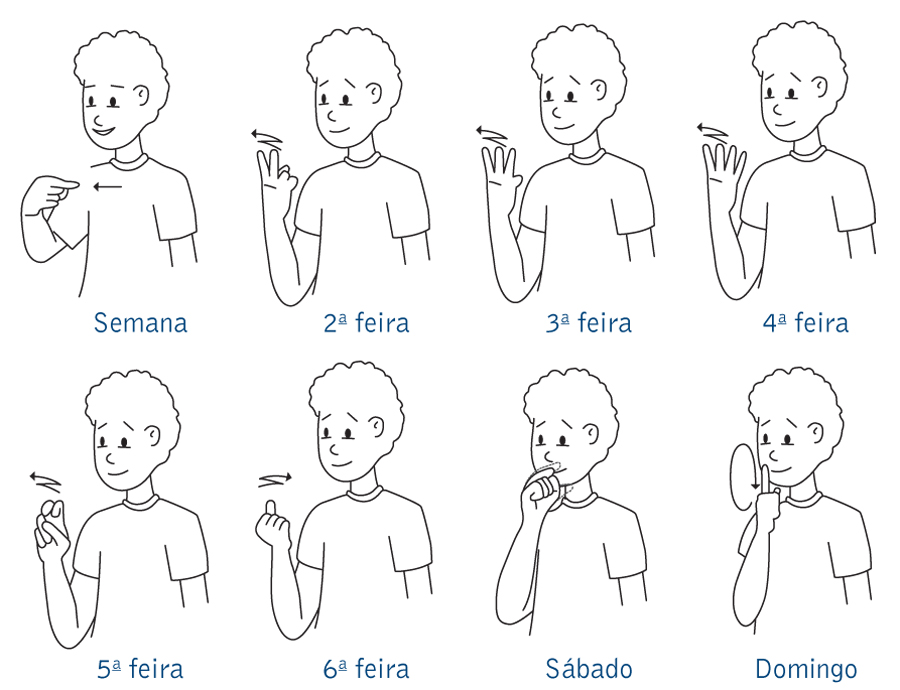
\includegraphics[width=0.8\textwidth]{images/libras-dias-semana.jpg}}
\caption*{Fonte: Centro de Educação para Surdos Rio Branco \url{www.ces.org.br}.}
\end{figure}

Considerando os parâmetros em questão, é possível ter uma dimensão da complexidade e capacidade linguística da Libras. Em particular, a \autoref{fig:libras-palavras} apresenta três palavras completamente distintas que compartilham a mesma CM (a letra ``L''). Entretanto, cada uma possui suas respectivas particularidades tendo em vista os parâmetros da Libras: (i) L: bochecha, M: semicircular para fora; (ii) L: testa, M: retilíneo repetido; e (iii) L: queixo, M: da articulação do dedo indicador -- abrir e fechar repetidamente.

\begin{figure}[htbp]
\centering
\caption{Libras: exemplos de sinais}
\label{fig:libras-palavras}
\begin{tabular}{ccc} 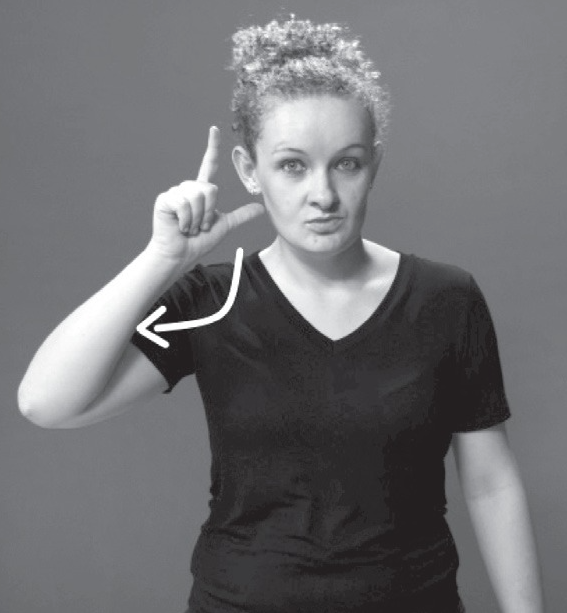
\includegraphics[width=0.331\textwidth]{images/libras-sinal-conseguir.png} &
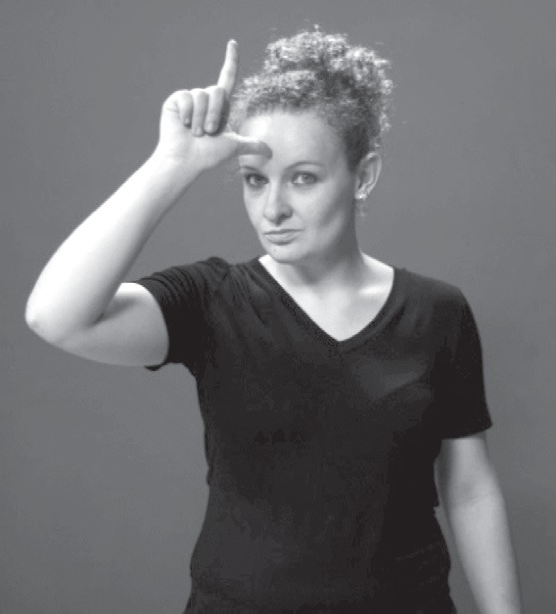
\includegraphics[width=0.325\textwidth]{images/libras-sinal-alemanha.png} & 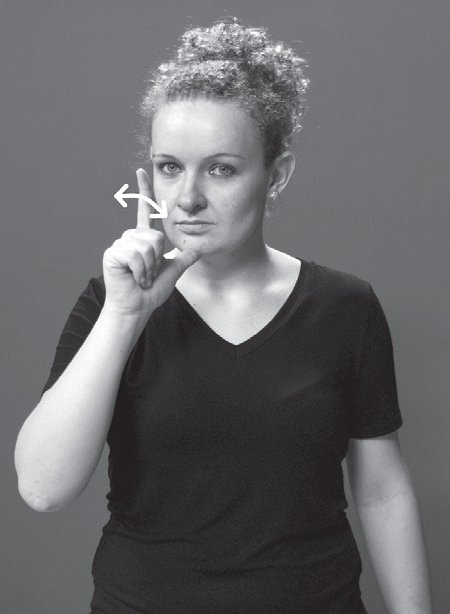
\includegraphics[width=0.264\textwidth]{images/libras-sinal-agua.png} \\
(i) Conseguir & (ii) Alemanha & (iii) Água \\
\end{tabular}
\caption*{Fonte: \citeonline{Quadros2019}}
\end{figure}

Adicionalmente, \citeonline{Quadros2019} apresenta uma visão mais técnica, na qual reitera formalmente que a Libras é uma língua dotada de todos os níveis de análise linguística. Tais características findam nossa discussão sobre a inegável integralidade da Libras enquanto língua:
\begin{itemize}
    \item Unidades mínimas (fonemas), que se combinam para formar palavras;
    \item Padrões prosódicos (realizados de forma não manual, através de expressões corporais ou faciais, por exemplo);
    \item Suas palavras se combinam para formar enunciados;
    \item Os enunciados apresentam proposições que podem ser analisadas do ponto de vista semântico, pragmático;
    \item Seus usos apresentam questões de ordem sociolinguística.
\end{itemize}

Sob outra perspectiva, levando em consideração o contexto social, as comunidades surdas brasileiras são representadas pela Federação Nacional de Educação e Integração de Surdos (FENEIS), que congrega várias instituições do país \cite{Quadros2019}. Uma das agendas da FENEIS era o reconhecimento legal da Libras, que culminou com a Lei nº 10.436/2002. Com isso, a Libras foi sancionada como língua de sinais oficial em 24 de Abril de 2002 \cite{Honora2017,Quadros2019,Cristiano2020}.

Segundo \citeonline{Quadros2019}, essa agenda fazia parte de um compromisso internacional estabelecido pela WFD, que inclui o reconhecimento legal das línguas de sinais de cada país. A FENEIS sempre esteve representada nas discussões em torno de questões relativas aos surdos, em especial, às políticas linguísticas voltadas para a Libras nos espaços governamentais.

Desde então, uma série de outras leis que regulamentam a Libras e assuntos relacionados à surdez vem sendo propostas. Nesse sentido, a \autoref{tab:libras:timeline} apresenta uma linha do tempo com as principais leis, decretos, portarias e resoluções sobre esses temas \cite{Cristiano2020}. Iniciativas como essas favorecem a inclusão social dos surdos, além de promover a democratização da educação inclusiva, apresentada em detalhes a seguir.

\begin{table}
\caption{Linha do tempo de leis sobre Libras e/ou Surdez.}
\label{tab:libras:timeline}
\centering
\begin{minipage}[t]{0.75\linewidth}
\color{gray}
\rule{\linewidth}{1pt}
\ytl{2002}{\href{https://www.libras.com.br/lei-10436-de-2002}{Lei nº 10.436}}
\ytl{2003}{\href{https://www.libras.com.br/portaria-3284-de-2003}{Portaria nº 3.284}}
\ytl{2004}{\href{https://www.libras.com.br/lei-10845-de-2004}{Lei nº 10.845}\\
\href{https://www.libras.com.br/lei-4304-de-2004}{Lei nº 4.304}\\
\href{https://www.libras.com.br/lei-4309-de-2004}{Lei nº 4.309}\\
\href{https://www.libras.com.br/projeto-de-lei-180-de-2004}{Projeto de Lei do Senado nº 180}}
\ytl{2005}{\href{https://www.libras.com.br/decreto-5626-de-2005}{Decreto nº 5.626}\\
\href{https://www.libras.com.br/lei-prolibras}{Prolibras}}
\ytl{2008}{\href{https://www.libras.com.br/resolucao-25-de-2008}{Resolução nº 25}\\
\href{https://www.libras.com.br/lei-11796-de-2008}{Lei nº 11.796}}
\ytl{2010}{\href{https://www.libras.com.br/lei-12319-de-2010}{Lei nº 12.319}\\
\href{https://www.libras.com.br/mensagem-532-de-2010}{Mensagem nº 532}\\
\href{https://www.libras.com.br/portaria-MEC-20-2010}{Portaria Normativa MEC 20/2010 – DOU: 08.10.2010}}
\ytl{2015}{\href{https://www.libras.com.br/lei-13146-de-2015}{Lei 13.146}}
\bigskip
\rule{\linewidth}{1pt}%
\end{minipage}%
\fautor
\end{table}

\subsection{Educação Inclusiva}
\label{fundamentacao-teorica:linguas-sinais:educacao-inclusiva}

Desde a década de 1990, surgem iniciativas globais de apoio a inclusão de PcD em escolas regulares. Em especial, a Declaração de Salamanca \cite{UNESCO1994} fomentou diretrizes básicas sobre a educação de alunos com deficiência nas escolas tradicionais para combater atitudes discriminatórias, visando uma sociedade mais inclusiva.

De acordo com a Declaração de Salamanca, o princípio fundamental da educação inclusiva é de que todos os alunos possam aprender juntos, independentemente de suas dificuldade e/ou diferenças. Por outro lado, tendo em vista a grande diversidade de PcD, essa é uma tarefa extremamente complexa, a qual exige uma nova postura tanto da gestão escolar quanto dos professores na busca de novos caminhos pedagógicos \cite{David2015}.

No Brasil, a atenção dada às minorias vem crescendo progressivamente nas últimas décadas, com o intuito de reduzir a exclusão social e proporcionar maior qualidade de vida. Em 2007, com o advento da ``Convenção dos Direitos das Pessoas com Deficiência'', os países signatários assumiram compromissos formais visando a educação inclusiva \cite{David2015,Quadros2019}. Como resultado, o Decreto nº 6.949/2009 (citado a seguir) foi estabelecido como uma referência para a criação de novas políticas públicas nesse contexto, as quais vêm adotando medidas para que:

\begin{quote}
\textit{``As PcD não sejam excluídas do sistema educacional geral sob alegação de deficiência e que as crianças com deficiência não sejam excluídas do ensino primário gratuito e compulsório ou do ensino secundário, sob alegação de deficiência:}
\begin{itemize}
    \item \textit{As PcD possam ter acesso ao ensino primário inclusivo, de qualidade e gratuito, e ao ensino secundário, em igualdade de condições com as demais pessoas na comunidade em que vivem;}
    \item \textit{Adaptações razoáveis de acordo com as necessidades individuais sejam providenciadas;}
    \item \textit{As PcD recebam o apoio necessário, no âmbito do sistema educacional geral, com vistas a facilitar sua efetiva educação;}
    \item \textit{Medidas de apoio individualizadas e efetivas sejam adotadas em ambientes que maximizem o desenvolvimento acadêmico e social, de acordo com a meta de inclusão plena.''}
\end{itemize}
\end{quote}

Em especial, a inclusão escolar foi formalizada no Brasil em 2008 por meio da ``Política Nacional de Educação Especial na Perspectiva Inclusiva''. Posteriormente, com a Lei Brasileira de Inclusão (LBI) em 2015, a conciliação da legislação nacional com a última ``Convenção dos Direitos das Pessoas com Deficiência'' (2011) estabeleceu legalmente as condições de implementação do sistema educacional inclusivo em todos os níveis e modalidades \cite{Alana2019}.

Por outro lado, o paradigma inclusivo, amparado pelas políticas nacionais, demonstrou a necessidade de uma profunda reestruturação do sistema educacional brasileiro. Essa reestruturação, que se propõem a atender a diversidade de seus alunos da melhor maneira possível, culminou projetos de uma escola para todos \cite{Almeida2015}. No que se refere à inclusão de pessoas com surdez, pode-se afirmar que há uma tensão explícita entre aqueles que defendem a presença dos alunos com surdez em escolas e classes tradicionais e aqueles que lutam pela educação de surdos em instituições bilíngues \cite{Almeida2015,Quadros2019}.

Segundo \citeonline{Almeida2015}, é importante esclarecer que aqueles que defendem o fim da educação especial de surdos e sua inserção nas escolas tradicionais, sem concentrá-los numa mesma turma, argumentam que insistir na educação de surdos é retroceder na inclusão e discriminar negativamente esses alunos. Entretanto, desconsideram diversas questões, tais como as linguísticas e culturais, intrínsecas à educação de surdos, e, também, a grande heterogeneidade presente em meio às pessoas com surdez.%, desde a polarização mais comum entre surdos, no sentido cultural do termo, e pessoas com deficiência auditiva e/ou ensurdecidas, até as demais diferenças sociais, físicas, etárias, étnicas e pessoais desses indivíduos.

\citeonline{Quadros2019} defende que, no caso específico dos surdos, ``inclusão'' deveria significar acesso à educação bilíngue, em que há agrupamentos de surdos, uso da língua de sinais, ensino da língua de sinais, ensino da língua portuguesa como segunda língua e a criação de um ambiente multilíngue e multicultural.

\citeonline{Quadros2019} e \citeonline{Almeida2015} concordam que os movimentos surdos clamam por inclusão em uma outra perspectiva. Nota-se que eles entendem a inclusão como garantia dos direitos de terem acesso à educação de fato, consolidada em princípios pedagógicos que estejam adequados aos surdos. Tais proposições ultrapassam as questões linguísticas, incluindo aspectos sociais, culturais, políticos e educacionais. Sendo assim, a educação bilíngue possui grande importância na concepção da educação inclusiva para surdos, pois trata a língua de sinais e a língua falada com o mesmo grau de importância no âmbito escolar. De acordo com \citeonline{Quadros2019}, os objetivos da educação bilíngue incluem os seguintes pontos:

\begin{enumerate}[label=(\alph*),noitemsep,topsep=0pt]
    \item Legitimar a experiência visual;
    \item Assegurar o desenvolvimento socio-emocional íntegro das crianças a partir da identificação com surdos adultos (encontro surdo-surdo);
    \item Criar um ambiente linguístico-social apropriado às formas particulares de processamento cognitivo e linguístico das crianças surdas;
    \item Garantir as possibilidades para que as crianças surdas construam uma teoria de mundo;
    \item Oportunizar o acesso à informação curricular e cultural.
\end{enumerate}

Nesse contexto, \citeonline{Quadros2019} discorre que sobre duas abordagens relevantes no âmbito da educação bilíngue com Libras, as quais, idealmente, devem coexistir em uma sala de aula inclusiva. Possibilitando assim, que surdos e ouvintes interajam naturalmente, tendo em vista as suas respectivas línguas principal (L1) e secundária (L2):
\begin{itemize}
    \item \textbf{Ensino de Libras como L1}: primeiramente, a carga horária para o ensino de Libras deve ser equivalente à carga horária da segunda língua (Português). Isso já integra a reestruturação da arquitetura escolar, pois as línguas passam a ocupar parte da carga horária de ensino de forma mais equivalente. Com isso, o aluno surdo será educado com ênfase na Libras, língua com a qual pode não ter tido contato prévio, geralmente porque ela não é a língua de convívio da maioria de seus familiares, o que caracteriza um desafio pedagógico adicional;
    \item \textbf{Ensino de Libras como L2}: para alunos ouvintes, familiares e demais pessoas envolvidas na comunidade escolar é um dos pilares da educação bilíngue, especialmente nas escolas inclusivas. Considerando um currículo no qual a Libras e a língua portuguesa compartilhem uma carga horária equivalente, os alunos ouvintes contarão com o ensino da Libras como segunda língua. A equivalência entre Libras e Língua portuguesa na distribuição da carga horária escolar é muito importante, pois legitima as duas línguas no espaço escolar ao lhes dar o mesmo status.
\end{itemize}

Por fim, \citeonline{Quadros2019} sintetiza o histórico das políticas públicas para a educação bilíngue em uma sequencia de acontecimentos fundamentais, muitos dos quais foram citados previamente. Para a autora, os seguintes eventos merecem destaque: (i) Lei ``da Libras'' nº 10.436/2002; (ii) Decreto nº 5.626/2005, (iii) Convenção dos Direitos das Pessoas com Deficiência (2007, 2011); (iv) Lei nº 13.005/2014 (que estabelece o Plano Nacional de Educação para o período de 2014-2024).

%Em 2018, após dez anos da Política, segundo o Censo Escolar, o número de matrículas da educação especial (na política de educação inclusiva do Brasil) chegou a 1,2 milhão, um aumento de 70\% desde 2008. Dentre as quais, o percentual de alunos incluídos em salas regulares, que em 2008 era de 54\%, passou para 92\% em 2018 \cite{Alana2019}.

A educação inclusiva representa um avanço no modo de conceber a escolarização de PcD, indicando os suportes educacionais necessários para operacionalizá-la. Em especial, no contexto dos surdos, a educação bilíngue surge como uma forma de inclusão da Libras como uma alternativa e não uma exceção. Entretanto, ainda existem muitos desafios e problemas para uma hipotética democratização das línguas de sinais, os quais são discutidos a seguir.

\subsection{Desafios e Problemas}
\label{fundamentacao-teorica:linguas-sinais:desafios}

Nesta seção alguns dos principais desafios das línguas de sinais e educação inclusiva são apresentados. Para isso, duas vertentes de discussão são delineadas: (i) Libras é língua de herança -- regionalidades e risco de extinção das línguas de sinais nacionais e locais; (ii) Educação inclusiva para todos -- alternativas para potencialização do ensino bilíngue em âmbito nacional. 

\citeonline{Quadros2019} discute as relações de pertencimento às comunidades surdas brasileiras e associa o termo ``língua de herança'' à Libras. Segundo \citeonline{Quadros2017}, a Libras é passada de geração em geração entre surdos de uma mesma comunidade (não necessariamente dentro do núcleo familiar). Além disso, é uma língua usada, principalmente, em grandes centros urbanos de um país que possui outra língua oficial, o Português, veiculado nos meios de comunicação, documentos oficiais, órgãos públicos etc. Sendo assim, a Libras é certamente uma língua de herança.

Nesse contexto, \citeonline{Quadros2019} expande essa discussão ao classificar as línguas de sinais em: nacionais e locais. Segundo a autora, as línguas de sinais locais são usadas por surdos geralmente de pequenas comunidades situadas em espaços geográficos específicos dentro de um mesmo país. Por outro lado, nacionais são as línguas usadas por várias comunidades surdas de um país, apresentando abrangência nacional. 

A Libras, por ser difundida em todo o território brasileiro, é considerada a língua de sinais nacional. Já as línguas de sinais locais, variam entre desligadas (isoladas), rurais e de vilas (incluindo as línguas de sinais indígenas, também locais e isoladas) \cite{Quadros2017,Quadros2019}. Nesse sentido, a autora discorre sobre uma maior possibilidade de extinção das línguas de sinais locais, principalmente devido a maior disseminação da Libras que, com o tempo, poderia se consolidar através das novas gerações e interromper a ``tradição'' das línguas locais.

A extinção de uma línguas de sinais, traz consigo uma perda social e cultural imensuráveis. Nesse contexto, \citeonline{Quadros2019} apresenta evidências de que a própria Libras está em risco, não obstantes seu reconhecimento por meio de lei e as várias políticas públicas para sua valorização. Tal risco decorre da forma de transmissão da Libras, o fato de não ser transmitida de pai para filho -- a maioria das crianças surdas nasce em famílias de ouvintes monolíngues -- torna a língua suscetível a constantes reinvenções. As crianças surdas crescem sem uma língua estabelecida. Em alguns casos, na tentativa de se comunicarem, elaboram produções próprias que podem se tornar verdadeiras línguas emergentes. No entanto, muitas vezes, terão contato tardio com uma língua de sinais já estabelecida, como a Libras.

De forma complementar, \citeonline{Quadros2019} alerta que existem políticas educacionais que inviabilizam a aquisição de linguagem através da Libras, quando não proporcionam o desenvolvimento da criança surda com seus pares (outras crianças surdas) e com referências de adultos surdos sinalizantes da Libras. Com isso, a criança surda só virá a ter contato com a Libras tardiamente, já com vários comprometimentos de ordem linguística e cognitiva. No período sem acesso à Libras, algumas crianças têm contato superficial com professores que sabem alguns sinais e, se tiverem sorte, com intérpretes de Libras. Nesse contexto, as crianças aprendem uma sinalização que não é propriamente uma língua, estabelecida a partir de modelos que apenas incorporam algo da Libras.

Portanto, podemos concluir que a Libras também está em risco, pois as crianças vão se tornar os adultos surdos de amanhã, e os adultos surdos sinalizantes da Libras irão morrer algum dia. O legado da Libras só será mantido se as crianças surdas tiverem contato com adultos surdos sinalizantes em Libras, pois a herança linguística é transmitida pela comunidade surda, não pelas famílias \cite{Quadros2019}.

Por outro lado, ao pensar na educação inclusiva, um dos grandes desafios que se apresentam é o atendimento a todos os indivíduo, de forma igualitária, no que se refere aos direitos à educação, e que valorize a diversidade como elemento que possibilite, a todo e qualquer indivíduo, com ou sem deficiências, as ferramentas necessárias para o seu aprendizado \cite{Almeida2015}.

\citeonline{Almeida2015} afirma que os modelos de escolarização impostos aos surdos, na maioria das vezes, os desconsideraram em sua especificidade. Adicionalmente, o autor critica a atual aplicação de propostas inclusivas, ditas bilíngues, que ``mantêm de forma velada a ideia de que o surdo precisa ser reabilitado e de que a Libras é apenas mais um recurso de acessibilidade''. Essa critica é extremamente pertinente e traz a tona a diferença fundamental entre os termos acessibilidade e inclusão, no contexto dos surdos. Nesse sentido, \citeonline{Quadros2019} discorre sobre esses conceitos, com o adendo do termo exclusão (\autoref{tab:glossario:acessibilidade-exclusao-inclusao}).

\begin{table}[htbp]
\caption{Glossário: Acessibilidade, Exclusão e Inclusão}
\label{tab:glossario:acessibilidade-exclusao-inclusao}
\begin{tabularx}{\textwidth}{l|X} \hline
Acessibilidade &  Tudo o que é acessível, ou seja, tudo o que as pessoas conseguem compreender, atender, aquilo de que conseguem participar efetivamente. \textbf{No caso dos surdos, a acessibilidade começa pela língua de sinais, que os inclui na conversa, na interação, no espaço social.} Há também outros aspectos a serem considerados para garantir a acessibilidade aos surdos. Um exemplo é o espaço, que precisa ser suficientemente iluminado para ser visto pelos surdos. Locais escuros os excluem. Sinais luminosos, em vez de sinais sonoros em espaços públicos e escolas são também outro exemplo de medidas que tornam o espaço acessível ao surdo.\\ \hline
Exclusão & Exclusão envolve a privação de alguém em participar de algumas atividades ou funções. No caso dos surdos, uma das formas mais contundentes de exclusão é o uso da língua falada. \textbf{Os surdos não ouvem a língua falada, então são facilmente excluídos do que está sendo tratado.} Para evitar a exclusão dos surdos em contextos em que se usa a fala como meio de comunicação, são contratados intérpretes de línguas de sinais, tornando assim o ambiente acessível. \\ \hline
\textbf{Inclusão} & \textbf{Inclusão é um termo usado para se referir à inserção das pessoas com deficiência (em certos contextos, abrange quaisquer pessoas que apresentem marcas sociais diferenciadas, tais como negros, homossexuais, mulheres, todas consideradas relativas do ponto de vista de quem estabelece o que seria a norma) na sociedade. O termo é comumente usado para se referir à ``educação inclusiva'' (\autoref{fundamentacao-teorica:linguas-sinais:educacao-inclusiva}), na qual os surdos são incluídos, idealmente, através do bilinguismo.} \\ \hline
\end{tabularx}
\caption*{Fonte: \citeonline{Quadros2019}.}
\end{table}

Com base nas definições de \citeonline{Quadros2019} e as discussões preestabelecidas neste trabalho, fica evidente que os surdos almejam a inclusão, além da acessibilidade, que fica implícita em um contexto inclusivo. Isso porque o fato de um ambiente ou solução ser acessível, não garante que o mesmo seja inclusivo. Por isso, é necessário refletir sobre estratégias e ferramentas que possam auxiliar na inclusão dos surdos, em especial no âmbito educacional. Tendo isso em mente, a seção seguinte fundamenta possíveis alternativas no conjuntura das tecnologias aplicadas à educação.

\section{Tecnologias da Informação e Comunicação (TICs)}
\label{fundamentacao-teorica:tic}

A educação e a busca por conhecimento representam, especialmente no contexto das PcD, algumas das formas mais efetivas para a inclusão social dessas pessoas. Esse cenário, associado ao rápido crescimento das Tecnologias de Informação e Comunicação (TICs), tem favorecido o surgimento de novas modalidades de ensino, proporcionando alternativas mais adequadas ao contexto de seus aprendizes na atual sociedade \cite{Kukulska2005, Castrillo2014}. 

Segundo a União Internacional de Telecomunicações (ITU), agência especializada nas TICs, pela primeira vez na história mais da metade da população mundial têm acesso à Internet, o equivalente a 4 bilhões de pessoas \cite{Itu2020}. Cronologicamente, o acesso individual à rede subiu de 17\% em 2005 para 51\% em 2019, um aumento expressivo que demostra uma forte tendência para um mundo totalmente conectado. De modo adicional, o ITU apresentou uma variação dessa estimativa considerando o público jovem (15 a 24 anos). Com isso, ficou evidente que esse grupo de pessoas é muito mais ativo com relação à Internet (\autoref{fig:itu-uso-internet}).

\begin{figure}[htbp]
\caption{ITU: Porcentagem de indivíduos que usam a Internet.}
\label{fig:itu-uso-internet}
\centerline{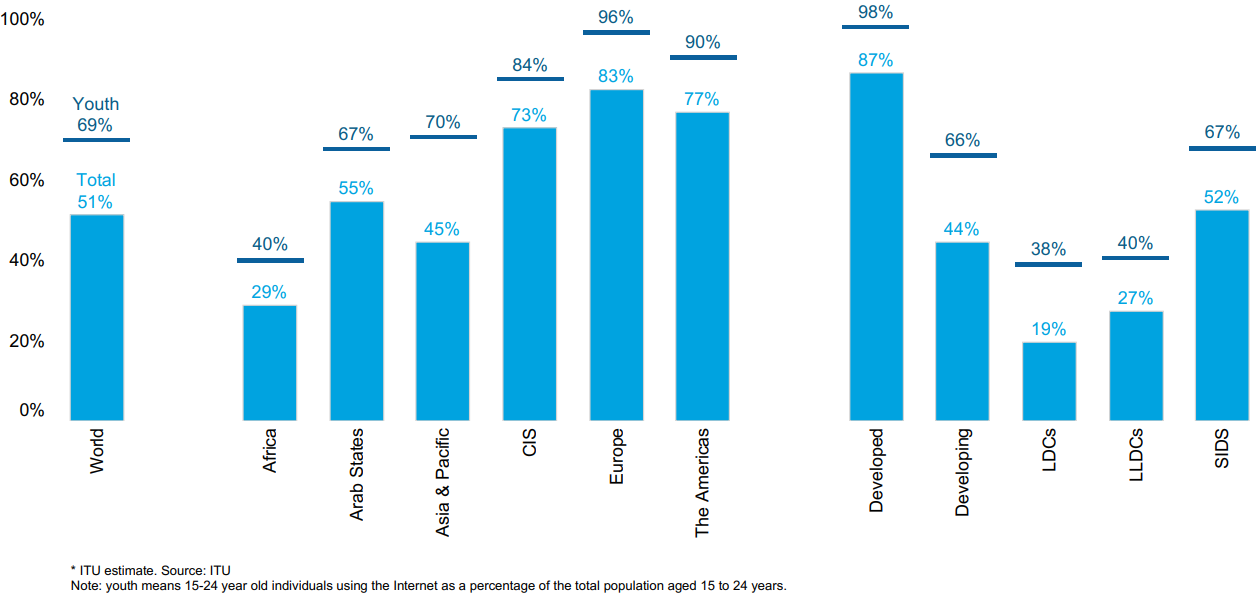
\includegraphics[width=1\textwidth]{images/itu-individuals-using-internet.png}}
\caption*{Fonte: \citeonline{Itu2020}}
\end{figure}

Vale ressaltar que as TICs não se limitam à soluções baseadas em Internet, muitas delas, inclusive, têm a capacidade de funcionar totalmente offline. Com isso, em cenários onde o acesso à Rede ainda é escasso (como em zonas rurais), também é possível promover o uso das TICs. Nesse sentido, de acordo com o último relatório do \citeonline{Itu2020}, em apenas 8 das 73 economias analisadas menos da metade da população possui um smartfone (\autoref{fig:itu-donos-smartfones}). No Brasil, por exemplo, estima-se que 80-89\% das pessoas possui ao menos um dispositivo.

\begin{figure}[htbp]
\caption{ITU: Porcentagem de indivíduos que possuem um smartfone.}
\label{fig:itu-donos-smartfones}
\centerline{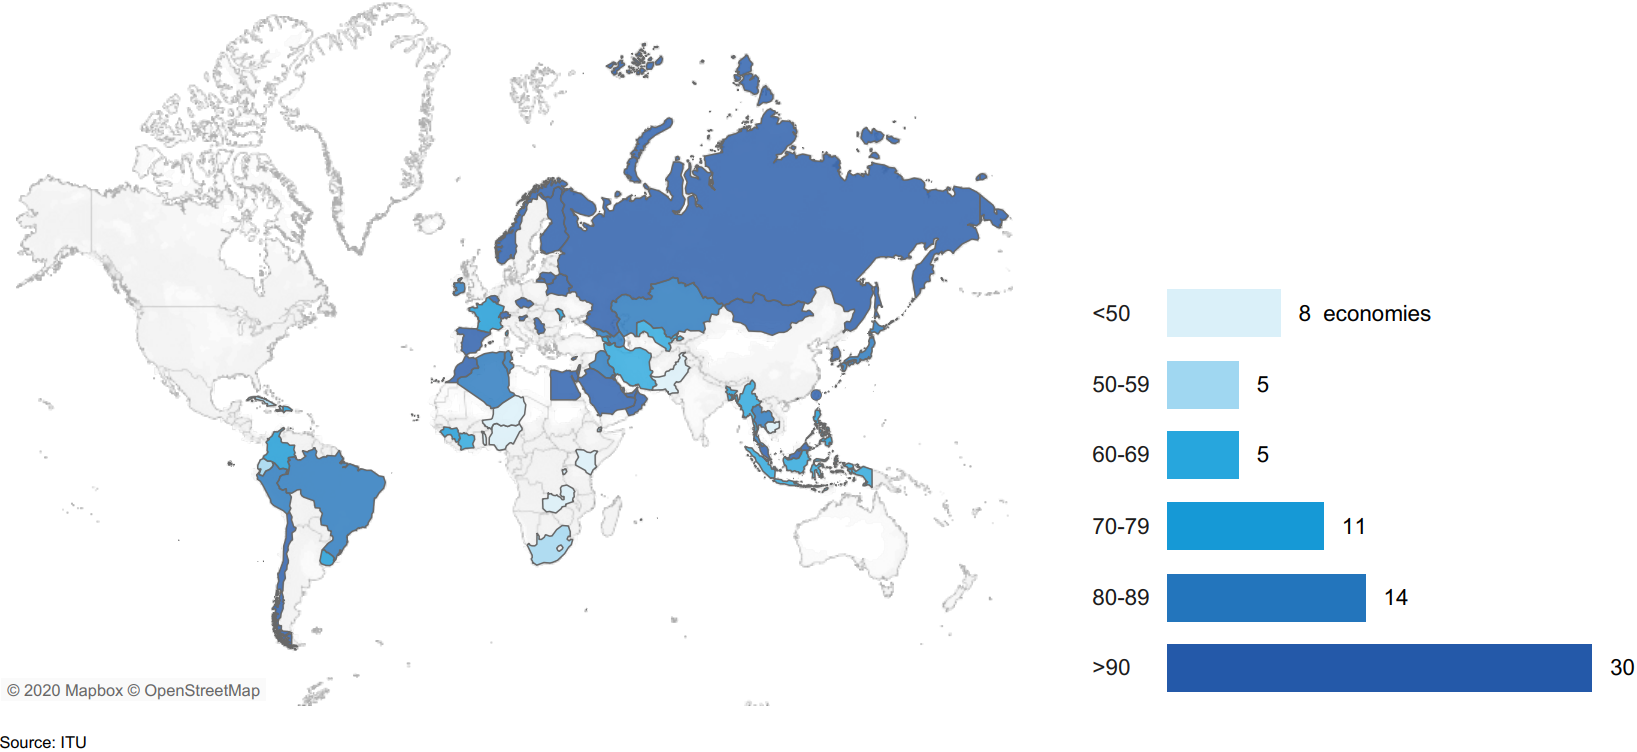
\includegraphics[width=1\textwidth]{images/itu-individuals-owning-mobile-phone.png}}
\caption*{Fonte: \citeonline{Itu2020}}
\end{figure}

Sendo assim, é possível inferir que o desenvolvimento de aplicativos móveis seria uma abordagem efetiva no Brasil. Além disso, é sabido que o público jovem é mais ativo no uso da Internet \cite{Itu2020}, o que pode servir de insumo para requisitos e especificações técnicas de soluções. Portanto, tais fatos podem direcionar de forma assertiva o desenvolvimento de aplicações adequadas ao contexto de seus usuários, especialmente no domínio educacional.%, visando o suporte às línguas oral e de sinais, por exemplo.

\subsection{Tecnologia e Educação}
\label{fundamentacao-teorica:tic:educacao}

\citeonline{Cilli2017} relatam que a educação no Brasil contou com vários tipos de abordagens desde o século XX, as quais se mesclavam em alguns momentos e se distanciavam em outros, mas em cada uma delas foram utilizadas as tecnologias disponíveis de acordo com a forma pela qual se acreditava que ocorria o processo de ensino-aprendizagem. Nesse contexto, \citeonline{Cilli2017} fundamentam as abordagens mais importantes historicamente nas seguintes:

\begin{itemize}
    \item \textbf{Tradicional}: Trata-se de uma concepção e uma prática educacional que persiste no tempo, em suas diferentes formas, na qual o adulto é considerado como um homem acabado, ``pronto'' e o aluno como um ``adulto em miniatura'', que precisa ser atualizado;
    \item \textbf{Comportamentalista}: Nessa abordagem o conhecimento é considerado uma nova descoberta para o aluno. Contudo, considera-se que esse novo conhecimento já se encontrava presente na realidade exterior do aluno. Em outras palavras, o ser humano é uma consequência das influências ou forças existentes no meio ambiente e, dessa forma, surge a hipótese de que o homem não é um ser livre, pois depende do conhecimento que já existe fora dele para sobreviver. Portanto, o conhecimento é o resultado direto da experiência, e o comportamento humano deve ser estruturado indutivamente , via experiência;
    \item \textbf{Humanista}: Enfatiza o papel do sujeito como principal elaborador do conhecimento humano. Propõe que o crescimento deve ser centrado no desenvolvimento da personalidade do indivíduo, na sua capacidade de atuar como uma pessoa integrada, uma vez que o homem é considerado como uma pessoa situada no mundo. Não existem modelos prontos nem regras a seguir, mas um processo de vir a ser . O objetivo do ser humano é a auto realização ou uso pleno de suas potencialidades e capacidades;
    \item \textbf{Sociocultural}: A partir das obras de Paulo Freire, enfatiza-se os aspectos sócio-político-culturais , havendo uma grande preocupação com a cultura popular. Cabe enfatizar que essa preocupação ocorre desde a II Guerra Mundial com um aumento crescente até nossos dias, uma vez que o homem está inserido no contexto histórico, o que indica que a ação educativa deve promover o indivíduo como sendo único dentro da sociedade a qual pertence;
    \item \textbf{Cognitivista}: Organização do conhecimento, a qual ocorre por meio do processamento de informações, dos estilos de pensamento ou estilos cognitivos e dos comportamentos relativos à tomada de decisões, dentre outros. Nesse sentido, o homem e mundo são analisados conjuntamente, já que o conhecimento é o produto da interação entre eles;
    \item \textbf{Teoria da Aprendizagem Significativa}: Processo pelo qual uma nova informação se relaciona de maneira não arbitrária e substantiva na estrutura cognitiva do aluno. Em outras palavras, ela não ocorre de forma literal, não é armazenada na memória da mesma forma que o aluno ouviu ou leu a informação;
    \item \textbf{Teoria das Inteligências Múltiplas}: Desenvolvida por Howard Gardner no início da década de 1980, na Universidade de Harvard, onde o autor é professor. Por meio dessa teoria foi possível identificar, de forma clara e objetiva, as necessidades atuais dos alunos em suas várias faixas etárias. Por isso, essa teoria é utilizada como embasamento na prática pedagógica de inúmeras escolas no mundo inteiro. De acordo com Gardner todos nós possuímos, pelo menos, nove tipos diferentes de inteligência, chamadas por ele de Inteligências Múltiplas. Vamos relembrar aqui que Inteligência diz respeito à forma como as pessoas resolvem problemas e interagem com a sociedade com a qual convivem:
    \subitem 1. \textit{Linguística ou verbal}: domínio e gosto pelos idiomas e pelas palavras.  Ex: poetas, escritores e linguistas;
    \subitem 2. \textit{Lógico matemática}:  capacidade de confrontar e avaliar objetos e abstrações. Facilidade para o raciocínio dedutivo e para solucionar problemas matemáticos. Ex: engenheiros, matemáticos, físicos;
    \subitem 3. \textit{Musical}: facilidade em reproduzir padrões musicais de ouvido além de discernir os diferentes timbres e ritmos. Ex: músicos, interpretes, compositores;
    \subitem 4. \textit{Visuespacial}: capacidade de compreender o mundo visual com precisão e reproduzi-los mentalmente mesmo sem estímulos físicos. Ex: arquitetos, escultores, cartógrafos, jogadores de xadrez;
    \subitem 5. \textit{Corporal cinestésica}: capacidade de controlar e orquestrar movimentos do corpo. Ex: atores, esportistas, dançarinos;
    \subitem 6. \textit{Intrapessoal}: capacidade de se conhecer. Ex: psicólogos, psicanalistas, neurologistas e conselheiro;
    \subitem 7. \textit{Interpessoal}: habilidade de entender as interações, motivações e desejos dos outros. Ex: políticos, religiosos, professores;
    \subitem 8. \textit{Naturalista}: sensibilidade para compreender e organizar os objetos, fenômenos e padrões da natureza, como reconhecer plantas, animais e minerais. Ex: geólogos, biólogos;
    \subitem 9. \textit{Existencial}: capacidade de refletir e ponderar sobre questões fundamentais da existência. Ex: Jean-Paul Sartre, Papa Francisco, Dalai Lama. 
\end{itemize}

Tendo em vista as abordagens em questão, \citeonline{Cilli2017} detalha cada um delas no contexto do uso da tecnologia como ferramenta de apoio ao processo ensino-aprendizagem. Desta forma, a \autoref{tab:abordagens-pedagogicas:tecnologia} foi idealizada com o objetivo de sintetizar tais tecnologias, as quais nem sempre são citadas diretamente, pois o conceito de tecnologia pode ser relativizado dependendo da abordagem.

\begin{table}[htbp]
\caption{Tecnologias/Recursos das abordagens pedagógicas}
\label{tab:abordagens-pedagogicas:tecnologia}
\begin{tabularx}{\textwidth}{p{3.5cm}|X} \hline
\textbf{Abordagem} & \textbf{Recursos/Tecnologias} \\ \hline
Tradicional & As tecnologias mais utilizadas são aquelas que permitem maior intensidade na concentração do aluno para que este possa memorizar a maior quantidade de informações possível. Por isso, os recursos de ensino mais utilizados são: \textbf{livro, caderno, lousa, e as ações do professor enquanto transmissor de informações}. \\ \hline
Comportamentalista & Recursos que permitem o uso de estimulo e resposta como o estudo dirigido e a instrução programada, cujos \textbf{materiais já trazem as respostas dos exercícios e tentam prever possíveis questionamentos que os alunos possam fazer a respeito do que estão aprendendo}, com base no comportamento dos mesmos. \\ \hline
Humanista & Qualquer tipo de recurso que facilite tanto o desenvolvimento racional como o emocional, e os brinquedos pedagógicos tem especial destaque nesse processo por serem capazes de simular situações de convívio com a família e com a sociedade em geral, permitindo assim com que o aluno se expresse e reconheça a importância da forma como essas expressões ocorrem, principalmente no que diz respeito a seu desenvolvimento emocional. Aqui estão presentes recursos como \textbf{fantoches, roupas para teatro, livros interativos, histórias contadas via meios digitais}. \\ \hline
Sociocultural & Recursos com os quais os alunos convivem no seu dia a dia, também podem ser considerados como recursos tecnológicos para a aprendizagem. Aqui podemos citar a \textbf{televisão, vídeos, imagens de realidades a serem entendidas}. \\ \hline
Cognitivista & Recursos tecnológicos como \textbf{computadores, tablets e smartfones} permitem com que os alunos participem de jogos digitais, pesquisas na Internet e construção de textos de forma colaborativa. \\ \hline
Teoria da Aprendizagem Significativa & Esta teoria nos inspira a refletir sobre a estrutura em que os diversos \textbf{conteúdos são desenvolvidos para que posteriormente sejam disponibilizados em recursos tecnológicos}, ou, então, de que forma o professor planejará as atividades para que todo o processo seja organizado de forma significativa e atenda aos objetivos propostos. \\ \hline
Teoria das Inteligências Múltiplas & Assim como a Teoria da Aprendizagem Significativa, nos estimula a analisar que tipo de conteúdo está sendo veiculado para a promoção do ensino e da aprendizagem. Contudo, no caso da Teoria das Inteligências Múltiplas, também podemos observar a qualidade das atividades que são propostas para garantir que os principais tipos de competências e habilidades realmente sejam contemplados no processo. \\ \hline
\end{tabularx}
\caption*{Fonte: \citeonline{Cilli2017}.}
\end{table}

Com isso, foi possível obter uma visão geral das principais abordagens pedagógicas existentes. Entretanto, elas devem se adaptar em muitos aspectos, visando a educação inclusiva, como visto anteriormente. Nesse sentido, para que a tecnologia possa apoiar tais abordagens em um contexto inclusivo, as tecnologias assistivas são fundamentais, pois potencializam o aprendizado de PcD. A seção a seguir trata desse tema em maiores detalhes.

\subsection{Tecnologia Assistiva}
\label{fundamentacao-teorica:tic:assistiva}

Segundo \citeonline{Bersch2017}, a Tecnologia Assistiva (TA) é um termo que identifica o conjunto de recursos e serviços que contribuem para proporcionar ou ampliar habilidades funcionais de PcD e consequentemente promover independência e inclusão. Já \cite{Cook2015} a define como uma ampla gama de equipamentos, serviços, estratégias e práticas concebidas e aplicadas para reduzir os problemas encontrados pelas PcD.

No Brasil, em 2006 foi instituído o Comitê de Ajudas Técnicas (CAT), estabelecido pelo Decreto nº 5.296/2004 no âmbito da Secretaria Especial dos Direitos Humanos da Presidência da República, com o objetivo de aperfeiçoar, dar transparência e legitimidade ao desenvolvimento da TA. No início, ``Ajudas Técnicas'' era um termo utilizado, mas atualmente foi descontinuado em detrimento da TA \cite{Cat2008}. De forma adicional, \citeonline{Cat2008} define a TA como:

\begin{quote}
``\textit{Uma área do conhecimento, de característica interdisciplinar, que engloba produtos, recursos, metodologias, estratégias, práticas e serviços que objetivam promover a funcionalidade, relacionada à atividade e participação, de PcD, incapacidades ou mobilidade reduzida, visando sua autonomia, independência, qualidade de vida e inclusão social.}''
\end{quote}

\citeonline{Bersch2017}, por sua vez, vem contribuindo consistentemente na área da TA. Nesse sentido, a autora propõem a classificação do conceito de TA em algumas categorias, as quais estão listadas a seguir, com destaque para a categoria destinada às recursos/serviços para surdos:

\begin{itemize}
\item Auxílios para a vida diária e vida prática;%:  Materiais e produtos para auxílio em tarefas rotineiras tais como comer, cozinhar, vestir-se, tomar banho e executar necessidades pessoais, manutenção da casa etc.
\item Comunicação Aumentativa e Alternativa (CAA);%:  Recursos, eletrônicos ou não, que permitem a comunicação expressiva e receptiva das pessoas sem a fala ou com limitações da mesma. Recursos como as pranchas de comunicação, construídas com simbologia gráfica (BLISS, PCS e outros), letras ou palavras escritas, são utilizados pelo usuário da CAA para expressar;
\item Recursos de acessibilidade ao computador;%:  Equipamentos de entrada e saída (síntese de voz, Braille), auxílios alternativos de acesso (ponteiras de cabeça, de luz), teclados modificados ou alternativos, acionadores, softwares especiais (de reconhecimento de voz, etc.), que permitem as pessoas com deficiência a usarem o computador.
\item Sistemas de controle de ambiente;%:  Sistemas eletrônicos que permitem as pessoas com limitações moto-locomotoras, controlar remotamente aparelhos eletro-eletrônicos, sistemas de segurança, entre outros, localizados em seu quarto, sala, escritório, casa e arredores.
\item Projetos arquitetônicos para acessibilidade;%:  Adaptações estruturais e reformas na casa e/ou ambiente de trabalho, através de rampas, elevadores, adaptações em banheiros entre outras, que retiram ou reduzem as barreiras físicas, facilitando a locomoção da pessoa com deficiência.
\item Órteses e próteses;%:  Troca ou ajuste de partes do corpo, faltantes ou de funcionamento comprometido, por membros artificiais ou outros recurso ortopédicos (talas, apoios etc.). Inclui-se os protéticos para auxiliar nos deficits ou limitações cognitivas, como os gravadores de fita magnética ou digital que funcionam como lembretes instantâneos.
\item Adequação postural;%:  Adaptações para cadeira de rodas ou outro sistema de sentar visando o conforto e distribuição adequada da pressão na superfície da pele (almofadas especiais, assentos e encostos anatômicos), bem como posicionadores e contentores que propiciam maior estabilidade e postura adequada do corpo através do suporte e posicionamento de tronco/cabeça/membros.
\item Auxílios de mobilidade;%:  Cadeiras de rodas manuais e motorizadas, bases móveis, andadores, scooters de 3 rodas e qualquer outro veículo utilizado na melhoria da mobilidade pessoal.
\item Auxílios para ampliação da função visual e recursos que traduzem conteúdos visuais em áudio ou informação tátil;%:  Auxílios para grupos específicos que inclui lupas e lentes, Braille para equipamentos com síntese de voz, grandes telas de impressão, sistema de TV com aumento para leitura de documentos, publicações etc.
\item \textbf{Auxílios para melhorar a função auditiva e recursos utilizados para traduzir os conteúdos de áudio em imagens, texto e língua de sinais.};%:  Auxílios que inclui vários equipamentos (infravermelho, FM), aparelhos para surdez, telefones com teclado — teletipo (TTY), sistemas com alerta táctil-visual, entre outros.
\item Mobilidade em veículos;%:  Acessórios e adaptações que possibilitam a condução do veículo, elevadores para cadeiras de rodas, camionetas modificadas e outros veículos automotores usados no transporte pessoal.
\item Esporte e Lazer.
\end{itemize}

Retomando o conceito de educação inclusiva, as TA são ferramentas importantes para que os surdos tenham alternativas em termos de acessibilidade e, idealmente, sejam incluídos em todos os sentidos. De acordo com \citeonline{Bersch2017}, no campo educacional, pode haver uma distinção sutil entre TA e tecnologia educacional. Para não haver dúvidas, a autora sugere que se façam três perguntas:

\begin{quote}

1. ``\textit{O recurso está sendo utilizado por um aluno que enfrenta alguma barreira em função de sua deficiência (sensorial, motora ou intelectual) e este recurso/estratégia o auxilia na superação desta barreira?}''

2. ``\textit{O recurso está apoiando o aluno na realização de uma tarefa e proporcionando a ele a participação autônoma no desafio educacional, visando sempre chegar ao objetivo educacional proposto?}''

3. ``\textit{Sem este recurso o aluno estaria em desvantagem ou excluído de participação?}''

\end{quote}

Tendo respostas afirmativas para as três questões, \citeonline{Bersch2017} afirma que o recurso pode ser classificado como TA, mesmo quando ele se denomina como tecnologia educacional. Isso porque, de modo geral, toda a TA é uma tecnologia educacional, desde que esteja no domínio da educação. Com isso, é possível identificar de forma simples soluções/ferramentas sob a perspectiva teórica correta.

Nesta subseção foi possível entender o conceito de TA e sua relação intrínseca com a educação inclusiva, pois a TA pode prover soluções robustas o suficiente para que sinalizantes e ouvintes possam interagir de forma mais legítima/inclusiva. Com isso, a seguir, discutimos um pouco sobre a perspectiva de desenvolvimento desta proposta, juntamente com seus desafios e eventuais problemas.

\subsection{Desafios e Problemas}
\label{fundamentacao-teorica:tic:desafios}

Talvez o maior desafio das TICs seja atingir a onipresença a nível global, pois em países desenvolvidos  essa etapa já está praticamente concluída, tendo em vista alguns parâmetros relevantes como o acesso à Internet e o uso de smartfones. Esse cenário, aliado a necessidade de democratizar a educação inclusiva/bilíngue para surdos, sugere uma linha de pesquisa interessante.

Por outro lado, as práticas pedagógicas também devem ser levadas em conta, pois fazem parte do processo de ensino-aprendizagem e, consequentemente, influenciarão em sua dinâmica social e cultural. Por isso, propor algo que seja adaptável para diferentes contextos educacionais é uma das premissas deste projeto.

Sendo assim, podemos concluir que, para a criação de ambientes educacionais mais inclusivos, é necessário levar em consideração uma série de aspectos. Primeiramente, tratar as línguas de sinais com a mesma importância da língua falada, favorecendo a diversidade e a disseminação da cultura surda. Nesse contexto, o uso de TICs é importante para que as práticas pedagógicas sejam devidamente apoiadas através de recursos educacionais efetivos, os quais, muitas vezes, se caracterizam como TA. Por fim, identificar o estado da prática, considerando o ensino e aprendizagem com línguas de sinais mediante o uso das TICs, tornou-se uma premissa importante para a continuidade deste trabalho. Assim, um estudo sistemático foi conduzido, o qual é descrito em detalhes na seção seguinte.

\section{Considerações Finais}
\label{fundamentacao-teorica:fim}

Ao fim desta seção foi possível obter uma visão geral sobre os temas que fundamental este trabalho. De modo geral, as línguas de sinais foram apresentadas, com ênfase na Libras e nas boas práticas da educação inclusiva identificadas na literatura. Além disso, reforçamos que a Libras, assim como qualquer outra língua, possui completude linguística e variações regionais/culturais, o que deve ser levado em conta para a inclusão efetiva dos surdos no contexto escolar, preferencialmente através da educação bilíngue (Libras/Português).

Em outra perspectiva, as TICs podem ser grandes aliadas para a desmistificação do processo de inclusão dos surdos. Isso porque essas tecnologias nunca estiveram tão presentes no nosso cotidiano, o que permite a reflexão sobre potenciais soluções de TA no contexto educacional, visando a sinergia e inclusão entre alunos sinalizantes e ouvintes.

Entretanto, essas são percepções iniciais, fundamentadas apenas com base nos conceitos apresentados nesta seção. Sendo assim, a seguir apresenta-se a condução de um Mapeamento Sistemático da Literatura, cujo objetivo é identificar o estado da prática com relação aos conceitos de: (i) línguas de sinais; (ii) ensino e aprendizagem; e (iii) tecnologias. Com isso, a presente discussão será formalmente delineada considerando questões de pesquisa cuidadosamente definidas para esta proposta.

\chapter{Tecnologia, Educação e Línguas de Sinais: Um Mapeamento Sistemático}
\label{chapter:mapeamento-sistematico}

\section{Considerações iniciais}
\label{ms:inicio}

Segundo \citeonline{Kitchenham2007}, existem duas abordagens principais para a condução de estudos sistemáticos de literatura. A primeira delas é a Revisão Sistemática (RS), definida como um estudo secundário que usa uma metodologia para identificar, analisar e interpretar todas as evidências relacionadas a uma questão de pesquisa com um escopo bem definido, de forma replicável e menos propensa a viés.

\citeonline{Kitchenham2007} também definem um segundo tipo de estudo, denominado Mapeamento Sistemático (MS), que tem como objetivo apresentar as evidências de um domínio de estudo em um alto nível de granularidade, agrupando as evidências encontradas em áreas de similaridade e geralmente identificando linhas de pesquisa em ascensão e/ou áreas com contribuições científicas escassas.

Adicionalmente, \citeonline{Petersen2015} mencionam que a técnica de MS é recomendada quando há a falta de estudos primários relevantes e de alta qualidade. O MS é recomendado, em detrimento de uma RS, quando o tópico for muito abrangente ou existam poucas evidências a serem coletadas em um domínio mais específico. Desta forma, como consideramos um escopo de pesquisa amplo (buscando a convergência entre três grandes áreas: tecnologia, educação e línguas de sinais), optou-se pela condução de um MS.

Especificamente, o MS descrito neste trabalho buscou verificar o cenário atual de pesquisas envolvendo temáticas que relacionem os conceitos de ensino e aprendizagem através das línguas de sinais mediante o uso de tecnologia. Para isso, algumas das principais diretrizes disponíveis na literatura foram utilizadas no desenvolvimento deste estudo \cite{Kitchenham2007,Zhang2011,Petersen2015}.

As seções a seguir apresentam todo processo de condução do MS. A \autoref{ms:conducao} apresenta os detalhes sobre o protocolo, execução, extração de dados e resultados, já as Seções \ref{ms:cenario-internacional} e \ref{ms:cenario-nacional} discutem os estudos primários sob as perspectivas internacional e nacional.

\section{Mapeamento Sistemático}
\label{ms:conducao}

As diretrizes de \citeonline{Kitchenham2007,Zhang2011,Petersen2015} foram consideradas na definição do protocolo de pesquisa e processo de condução deste MS. Lembrando que um MS tem por objetivo evidenciar lacunas para, por exemplo, endossar futuras RS e/ou identificar linhas de pesquisa emergentes \cite{Kitchenham2007}. Além disso, por meio de uma categorização, o mapeamento fornece um resumo visual e conciso sobre uma determinada área ou temática \cite{Petersen2008}.

Segundo \citeonline{Nakagawa2010}, o primeiro e mais importante passo para obter sucesso em um MS é planejá-lo corretamente. Desta forma, com base nas diretrizes citadas previamente, definimos um protocolo que explorou estrategicamente cada uma das diretrizes \cite{Kitchenham2007,Zhang2011,Petersen2015}.

Nesse sentido, a abordagem proposta por \citeonline{Zhang2011} tem maior destaque neste MS, pois nossa estratégia de busca e critérios de qualidade se basearam nas diretrizes propostas pelos autores. A \autoref{ms:zhang-approach} sintetiza a abordagem de pesquisa sistemática em questão, a qual foi sutilmente adaptada para este estudo, visando aumentar o rigor do processo de pesquisa através do conceito do \textit{Quasi-Gold Standard} (QGS) em conjunto com algumas das boas práticas propostas pelas diretrizes de \citeonline{Kitchenham2007} e \citeonline{Petersen2015}.

\begin{figure}[htbp]
\caption{Busca sistemática baseada em QGS.}
\label{ms:zhang-approach}
\centerline{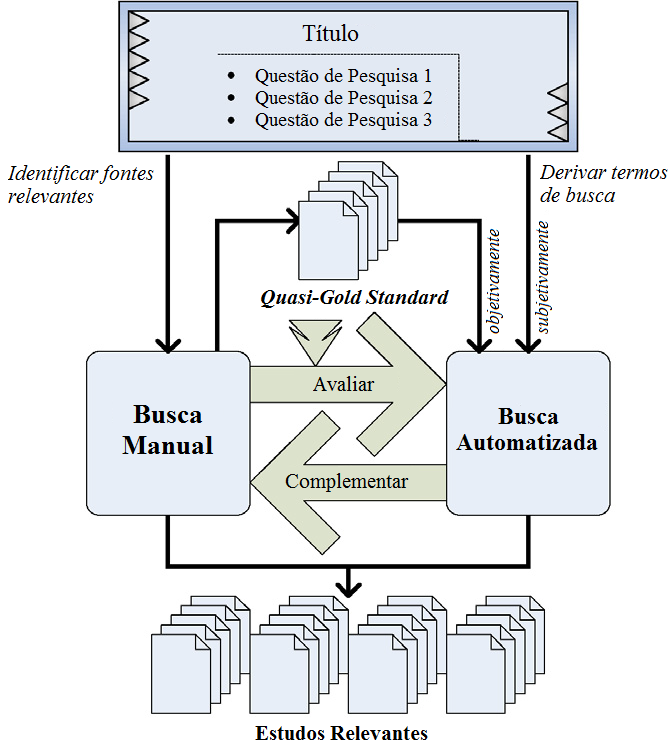
\includegraphics[width=0.55\textwidth]{images/zhang-systematic-mapping-approach.png}}
\caption*{Fonte: \citeonline{Zhang2011}.}
\end{figure}

Considerando a \autoref{ms:zhang-approach} é possível interpretar, em alto nível, a dinâmica da abordagem de \citeonline{Zhang2011}. Primeiramente, as questões de pesquisa devem ser definidas, juntamente com seus respectivos critérios de seleção (Subseções \ref{ms:conducao-escopo} e \ref{ms:conducao-busca}). Em seguida, as fontes para a busca manual (\autoref{ms:conducao-busca-manual}) e os termos para a busca automatizada (\autoref{ms:conducao-busca-automatizada}) são identificados/derivados. Com isso, o processo de busca manual define um conjunto de estudos primários relevantes, chamado de QGS. Através do QGS, a busca automatizada é avaliada e, se necessário, novas iterações podem ser realizadas (com o objetivo de refinar a busca automatizada) até que a qualidade seja considerada adequada pelo cálculo da \textit{quasi-sensitivity} (\autoref{ms:zhang-approach-steps}), mais detalhes na Subseção \ref{ms:conducao-busca-performance}. Por fim, os estudos selecionados pela busca automatizada, juntamente com o QGS (definido na busca manual), são classificados como relevantes/primários possibilitando a extração dos dados com o objetivo de responder às questões de pesquisa (Subseções \ref{ms:conducao-extracao-dados} e \ref{ms:resultados}).

\begin{figure}[htbp]
\caption{Etapas busca sistemática baseada em QGS.}
\label{ms:zhang-approach-steps}
\centerline{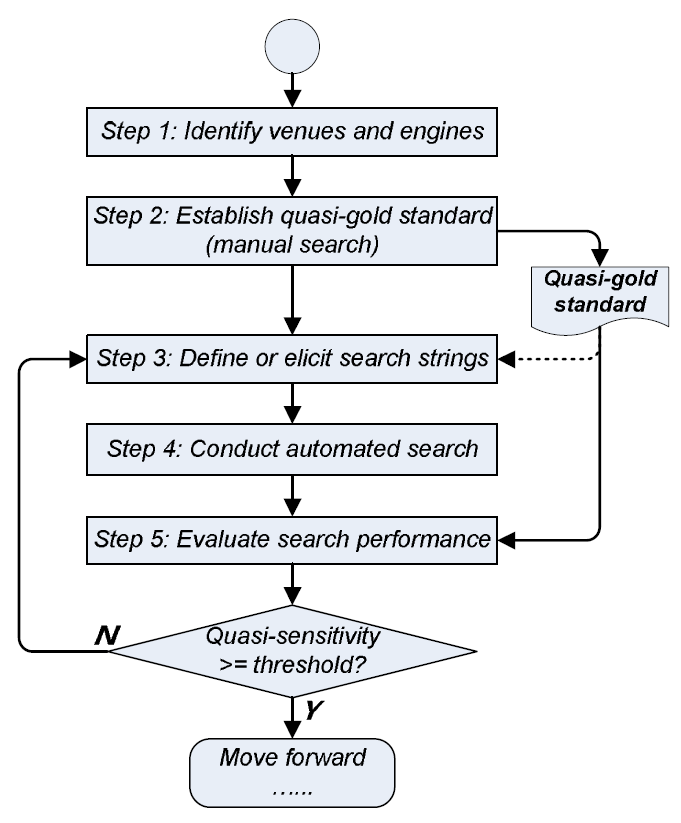
\includegraphics[width=0.55\textwidth]{images/zhang-systematic-mapping-steps.png}}
\caption*{Fonte: \citeonline{Zhang2011}.}
\end{figure}

\subsection{Definição do Escopo}
\label{ms:conducao-escopo}

As Questões de Pesquisa (QP) são essenciais para definir o escopo e identificar possíveis palavras-chave em um estudo sistemático de literatura \cite{Kitchenham2007,Petersen2015}. Neste contexto, uma abordagem comumente usada se dá através da aplicação dos critérios de PICO. Segundo \citeonline{Petticrew2008}, as QP podem ser estruturadas sob quatro aspectos: \textit{Population} (População); \textit{Intervention} (Intervenção); \textit{Comparison} (Comparação); e \textit{Outcome} (Resultados). Os critérios de PICO são apresentados na \autoref{table:pico}.

\begin{table}[!ht]
\caption{Critérios de PICO.}
\label{table:pico}
\centering
\begin{tabular}{ll}
\toprule
\textbf{\textit{Population}} & Alunos/Aprendizes de línguas de sinais. \\
\textbf{\textit{Intervention}} & Tecnologias relevantes para o ensino por meio das línguas de sinais. \\
\textbf{\textit{Comparison}} & Não se aplica. \\
\textbf{\textit{Outcome}} & Panorama tecnológico sobre o ensino baseado em línguas de sinais. \\ 
\bottomrule
\end{tabular}
\fautor
\end{table}

Através dos critérios definidos no PICO é possível identificar, de forma abstrata, o escopo do MS proposto. Sendo assim, o objetivo deste MS é determinar como a tecnologia está sendo aplicada no ensino e aprendizagem baseado em línguas de sinais, o que derivou as seguintes QP:

\begin{itemize}
    \item \textbf{QP1}: Quais áreas de desenvolvimento estão pesquisando sobre o ensino e aprendizagem através das linguagens de sinais?
    \begin{itemize}
        \item Quais são os tipos de soluções propostas (software ou hardware ou teóricas)?
        \item Quais tecnologias foram usadas?
        \item Quais métodos de avaliação foram aplicados?
    \end{itemize}
    \item \textbf{QP2}: Quais tópicos educacionais são abordados?
    \item \textbf{QP3}: Quais línguas de sinais são abordadas?
    \begin{itemize}
        \item Quais estudos abordam múltiplas línguas de sinais?
    \end{itemize}
\end{itemize}

De acordo com  \citeonline{Kitchenham2007}, um dos objetivos de um MS é realizar um levantamento de estudos relevantes para avaliar a quantidade de evidências existentes, visando responder as questões de pesquisa propostas. Segundo \citeonline{Felizardo2012}, o processo precisa ser rigoroso e imparcial, além de envolver uma ampla cobertura de fontes de informação, como bancos de dados, periódicos e conferências. Para minimizar o viés e maximizar o número de estudos examinados, é necessária uma estratégia de busca bem definida. A seguir, apresentamos em mais detalhes nossa abordagem de pesquisa, juntamente com seus critérios de seleção e avaliação da qualidade.

\subsection{Critérios de Seleção}
\label{ms:conducao-busca}

Segundo \citeonline{Kitchenham2007,Petersen2015}, os estudos sistemáticos requerem critérios explícitos de inclusão e exclusão para avaliar seus potenciais estudos primários. Assim, definimos os seguintes critérios de seleção:

\begin{itemize}
    \item Critério de Inclusão:
    \begin{itemize}
        \item Os estudos apresentam contribuições (software ou hardware ou teóricas) para o ensino e a aprendizagem de línguas de sinais.
    \end{itemize}
    \item Critérios de Exclusão:
    \begin{itemize}
        \item Estudos que não foram publicados no período de 2000 a 2019, seguindo um racional semelhante à \citeonline{Radermacher2013,Scatalon2019}, os quais sugerem que estudos anteriores a 2000 não representam as abordagens educacionais atuais, especialmente considerando o contexto da Engenharia de Software (ES);
        \item Estudos que não estão no campo da ES;
        \item Estudos classificados como resumos, resumos de conferências/editoriais, literatura cinza ou capítulos de livros;
        \item Estudos não apresentados em inglês ou português;
        \item Estudos não acessíveis em texto completo;
        \item Estudos duplicados ou superficialmente complementares de outros estudos.
    \end{itemize}
\end{itemize}

Ainda se tratando sobre os critérios de exclusão, consideramos necessários alguns esclarecimentos. Primeiro, escolhemos o inglês e o português, porque o primeiro é o idioma mais indexado pelos mecanismos de busca e o segundo é o idioma nativo dos autores. Além disso, pretendemos obter uma visão geral das contribuições em português. Por fim, entendemos como ``estudos não acessível em texto completo'' os trabalhos não cobertos por nosso acesso institucional. Com isso, estudos pagos e/ou inacessíveis, foram desconsiderados.

A seguir, apresentamos nossa busca manual e seus respectivos estudos selecionados que, por definição, representariam nosso QGS. Entretanto, a \autoref{ms:conducao-busca-manual} discorre sobre decisões importantes com relação à composição do QGS, pautadas principalmente pela grande diferença na qualidade de indexação entre as fontes nacionais e internacionais. Com isso, nosso QGS foi composto majoritariamente por estudos selecionados internacionalmente. Assim, a coesão entre a nossa estratégia de busca manual e a abordagem de \citeonline{Zhang2011} se mostrou mais adequada.

\subsection{Busca Manual}
\label{ms:conducao-busca-manual}

Para a etapa de busca manual, selecionamos fontes (periódicos e conferências) com ênfase em ES e educação. As fontes nacionais e internacionais foram definidas com o apoio de especialistas em ES do LabES\footnote{Laboratório de Engenharia de Software do ICMC--USP}. Nesta etapa, o conjunto \textit{title-abstract-keywords} foi utilizado para a avaliação dos estudos. De modo adicional, eventualmente outras seções foram lidas, visando uma classificação mais assertiva com base nos critérios de seleção propostos.

A \autoref{ms:table:busca-manual-nacional} apresenta as conferências e periódicos nacionais considerados durante a busca manual. Entretanto, os estudos obtidos dessas fontes foram desconsiderados na composição do QGS, pois a maioria das conferências/periódicos brasileiros não são indexados pelos mecanismos de busca internacionais e isso reduziria consideravelmente a eficácia da abordagem de busca sistemática baseada em QGS \cite{Zhang2011}. Todavia, os 46 estudos primários selecionados em fontes brasileiras serão devidamente discutidos nos resultados deste MS. 

\begin{table}[htbp]
\centering
\caption{Busca manual nacional}
\label{ms:table:busca-manual-nacional}
\begin{tabular}{lcc}
\hline
\textbf{Conferências/Periódicos} & \textbf{Fonte} & \textbf{Selecionados} \\ \hline
DesafIE                          & CEIE           & -                     \\
JAIE                             & CEIE           & -                     \\
RBIE                             & CEIE           & 2                     \\
RENOTE                           & CINTED         & 13                    \\
SBIE                             & CEIE           & 13                    \\
WAVE2                            & CEIE           & -                     \\
WCBIE                            & CEIE           & 11                    \\
WIE                              & CEIE           & 7                     \\
\multicolumn{2}{l}{\textbf{Total}}                & \textbf{46}           \\ \hline
\end{tabular}
\fautor
\end{table}

Por outro lado, a \autoref{ms:table:busca-manual-internacional} apresenta as conferências e periódicos internacionais considerados durante a busca manual. Essa etapa resultou na seleção de 19 estudos primários, que representam o QGS deste MS. Considerando as Bibliotecas/Editoras em questão, todas as fontes relevantes (com ao menos um estudo selecionado) podem ser obtidas pelas seguintes fontes: ACM (ACM Digital Library), IEEE (IEEE Xplore), Elsevier (ScienceDirect) e Springer (Springer Link). Sendo assim, de acordo com \citeonline{Zhang2011}, é apropriado que essas mesmas bases de dados sejam utilizadas para executar a busca automatizada, gerando assim uma sinergia maior com o QGS.

\begin{table}[htbp]
\centering
\caption{Busca manual internacional (QGS)}
\label{ms:table:busca-manual-internacional}
\begin{tabular}{lcc}
\hline
\textbf{Conferência/Periódico} & \textbf{Fonte}     & \textbf{Selecionados (QGS)} \\ \hline
ACM TOCE                       & ACM                & 0            \\ 
Computers \& Education         & Elsevier           & 5            \\ 
FIE                            & IEEE               & 0            \\ 
HCI International              & Springer           & 5            \\ 
ICALT                          & IEEE               & 5            \\ 
IEEE Trans. Educ.              & IEEE               & 1            \\ 
IEEE Trans. Learn. Technol.    & IEEE               & 0            \\ 
Informatics in Education       & Vilnius University & 0            \\ 
ITiCSE                         & ACM                & 2            \\ 
Learning @ Scale               & ACM                & 0            \\ 
SIGCSE                         & ACM                & 1            \\ 
\textbf{Total}                 & \textbf{}          & \textbf{19}  \\ \hline
\end{tabular}
\fautor
\end{table}

Por fim, em atenção a abordagem de busca sistemática baseada em QGS, se faz necessário esclarecer algumas definições. Primeiramente, o termo \textit{Gold Standard} representa todos os estudos primários possíveis de uma questão de pesquisa, ou seja, algo difícil de se obter. Por outro lado, o QGS representa um subconjunto desses estudos, se tornando uma alternativa mais viável \cite{Zhang2011}. Portanto, \citeonline{Zhang2011} sugerem a criação do QGS a partir dos estudos selecionados pela busca manual (\autoref{ms:table:busca-manual-internacional}), com o objetivo de aferir a qualidade da busca automatizada. Para isso, utilizamos a \textit{quasi-sensitivity}, uma formula que avalia o desempenho da busca automatizada, que deve incluir idealmente a maior parte dos estudos do QGS. 

A seção a seguir apresenta maiores detalhes sobre a condução da busca automatizada, tendo em vista as bases de dados e estudos relevantes (QGS) identificados através do processo de busca manual supracitado. Além disso, o processo de avaliação de performance da busca automatizada através da \textit{quasi-sensitivity} é devidamente detalhado.

\subsection{Busca Automatizada}
\label{ms:conducao-busca-automatizada}

Antes de realizar uma busca automatizada, é essencial definir os critérios para criação de uma string de busca. Nesse sentido, duas estratégias para identificação de palavras-chave foram utilizadas em conjunto: (i) análise do PICO e suas respectivas QP; (ii) importação da tripla \textit{title-abstract-keywords} em um software de análise de frequência. Os resultados desse processo produziram a seguinte string de busca:

\begin{center}
    (\textit{learn} \textbf{OR} \textit{learning} \textbf{OR} \textit{teach} \textbf{OR} \textit{teaching}) \textbf{AND}\\
    (``\textit{sign language}'' \textbf{OR} ``\textit{signed language}'') \textbf{AND}\\
    (\textit{technology} \textbf{OR} \textit{technologies})\\
\end{center}

Seguindo a proposta de \citeonline{Zhang2011}, realizamos a busca automatizada nas quatro bases de dados identificadas como relevantes pela busca manual: ACM Digital Library\footnote{https://dl.acm.org}, IEEE Xplore\footnote{https://ieeexplore.ieee.org}, ScienceDirect\footnote{https://sciencedirect.com}, Springer Link\footnote{https://link.springer.com}. Portanto, a string de busca em questão foi executada nessas máquinas de busca.

A \autoref{method:table:automated-search} resume os resultados da busca automatizada, onde a seleção dos estudos seguiu o mesmo racional apresentado na busca manual. Além disso, nossa busca automatizada retornou a maioria dos estudos selecionados pela busca manual (QGS), o que sugere uma boa sensibilidade da nossa string de busca. Nesse sentido, mais detalhes são discutidos na seção a seguir.

\begin{table}[htbp]
\centering
\caption{Resultados da busca automatizada}
\label{method:table:automated-search}
\begin{tabular}{lllll}
\hline
 &  & Busca Final &                 &                   \\ \cline{3-5} 
Base de Dados & \textbf{QGS} & Recuperados    & \textbf{no QGS} & \textbf{Relevantes} \\ \hline
ACM DigitalLibrary & 3            & 922          & 3               & 47                \\
IEEE Xplore        & 6            & 359          & 5               & 59                \\
ScienceDirect      & 5            & 1,961        & 5               & 20                \\
SpringerLink       & 5            & 4,980        & 5               & 36                \\
\textbf{Total}   & \textbf{19}  & 8,222        & \textbf{18}     & \textbf{162}      \\ \hline
\end{tabular}
\fautor
\end{table}

\subsubsection{Avaliação de Performance da Busca Automatizada}
\label{ms:conducao-busca-performance}

Segundo \citeonline{Zhang2011}, a qualidade da busca automatizada de uma pesquisa cientifica pode ser avaliada usando critérios consolidados na literatura, como a sensibilidade e a precisão. Nesse sentido, os autores propõem o conceito de \textit{quasi-sensibilidade}, uma derivação da sensibilidade tradicional que incorpora o QGS como critério de qualidade (\autoref{method:equation:quasi-sensitivity}).

\begin{equation}
\label{method:equation:quasi-sensitivity}
\text{\textit{quasi-sensibility}} = \frac{\text{\textit{Estudos relevantes recuperados (\textbf{no QGS})}}}{\text{\textit{Total de estudos relevantes (\textbf{QGS})}}}
\end{equation}

Portanto, para avaliar o desempenho da busca automatizada, calculamos a \textit{quasi-sensitivity} considerando os dados da \autoref{method:table:automated-search}. De acordo com \citeonline{Zhang2011}, quando o desempenho da pesquisa é aceitável (quase sensibilidade $\geq$ 80\%), os resultados da busca automatizada podem ser mesclados com o QGS e o processo de busca é finalizado (\autoref{ms:zhang-approach-steps}).

Como resultado, a \textit{quasi-sensitivity} foi calculada em 94,74\% (18/19), ou seja, o desempenho da pesquisa é aceitável \cite{Zhang2011}. Portanto, os 163 artigos selecionados pelas buscas manual e automatizada são potenciais estudos primários, portanto devem ser lidos na íntegra. Nesta etapa, 24 estudos foram excluídos de acordo com os critérios de inclusão e exclusão pré-estabelecidos. A \autoref{method:figure:evaluation-refinement} organiza nossos 139 estudos primários, tendo em vista a abordagem de busca sistemática baseada em QGS.

\begin{figure}[htbp]
\caption{Resultados da busca sistemática baseada em QGS.}
\label{method:figure:evaluation-refinement}
\centerline{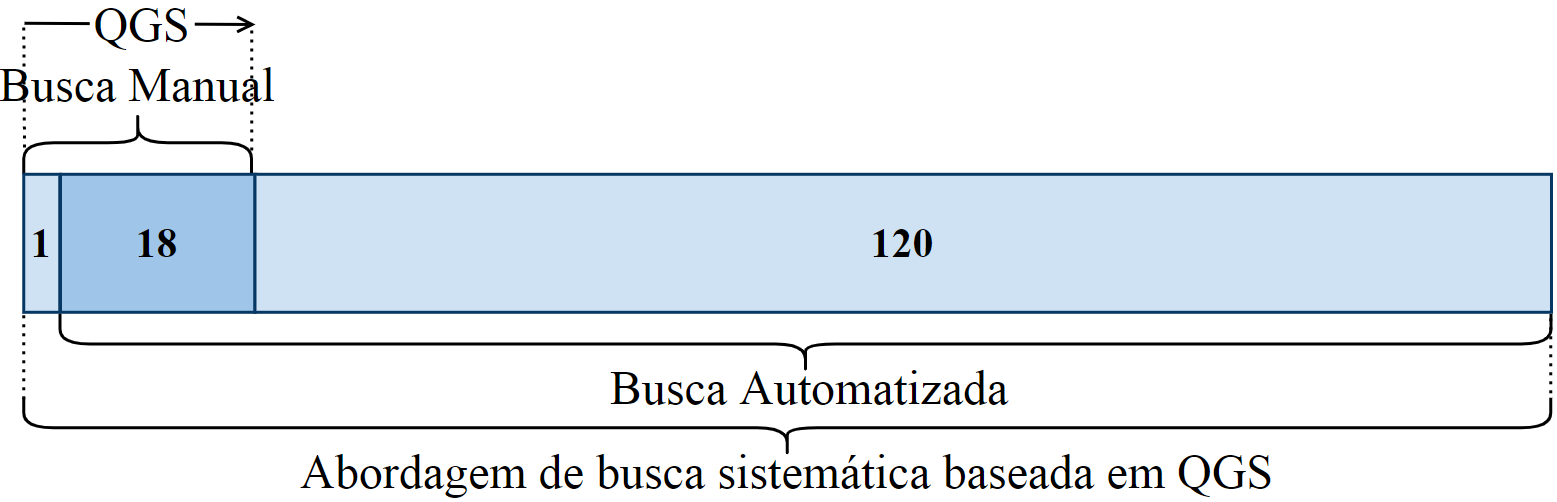
\includegraphics[width=0.8\textwidth]{images/systematic-mapping.png}}
\fautor
\end{figure}

\subsection{Extração de Dados}
\label{ms:conducao-extracao-dados}

Para extrair as informações relevantes dos estudos primários identificados, criamos um formulário de extração de dados. O modelo na \autoref{method:table:data-extraction} descreve as informações extraídas e apresenta seu relacionamento com cada QP, quando aplicável.

\begin{table}[htbp]
\centering
\caption{Formulário de extração de dados}
\label{method:table:data-extraction}
\begin{tabular}{lll}
\hline
\textbf{Item} & \textbf{Descrição} & \textbf{QP} \\ \hline
\textit{\textbf{Informações Gerais}} & & \\ \hline
ID & Identificador (prefixos \textit{INT} ou \textit{BRA}). & \\
Título & Título do estudo. & \\
Autores & Nomes dos autores. & \\
Ano & Ano de publicação do artigo. & \\
Conferência/Periódico & Nome do meio de publicação. & \\
Tipo de busca & Manual; Automatizada; Ambas. & \\
Língua & Inglês; Português. & \\
País & País da afiliação do primeiro autor. & \\ \hline
\textit{\textbf{Informações Específicas}} & & \\ \hline
Área da ES & Área de conhecimento da ES (SWEBOK). & QP1 \\
Tipo de solução & Software; Hardware; Teórica. & QP1 \\
Estratégia empírica & Quais estratégias empíricas foram encontradas. & QP1 \\
Tópico educacional & Quais tópicos educacionais foram encontrados. & QP2 \\
Línguas de sinais & Quais línguas de sinais foram encontradas. & QP3 \\ \hline
\end{tabular}
\fautor
\end{table}

Devido ao grande número de estudos primários selecionados no MS, optou-se por não incluir todas as referências explicitamente neste trabalho. Sendo assim, todos os artigos e seus respectivos dados (incluindo um glossário para o formulário de extração de dados) estão disponíveis online\footnote{\url{https://bit.ly/SM-DataExtraction}}.

Os estudos primários oriundos de eventos \textit{Internacionais} -- 139 publicações selecionados por meio da abordagem de busca sistemática baseada em QGS; e \textit{Brasileiros} -- 46 publicações selecionadas por meio da busca manual nacional, foram devidamente identificados pelos prefixos \textit{INT} e \textit{BRA}. Assim, um total de 185 estudos primários foram identificados pelo MS, os quais serão apresentados e discutidos nas seções a seguir.

\subsection{Resultados}
\label{ms:resultados}

Considerando os 185 estudos primários selecionados pelo MS, as informações mais relevantes para as QP foram sintetizadas seguindo a estrutura do formulário de extração de dados. Assim, nesta seção cada questão de pesquisa será abordada individualmente, evidenciando suas respectivas constatações. Antes disso, com base na análise de informações essenciais dos estudos, alguns cenários adicionais interessantes foram identificados. Com isso, foi possível estender os resultados deste MS por meio de informações transcendem as QP apresentadas.

Primeiramente, considerando a quantidade de publicações por ano, identificamos uma linha de tendência linear crescente (\autoref{results:figure:publications-year}). Portanto, é estatisticamente possível que este domínio de pesquisa esteja em ascensão globalmente. Além disso, o número reduzido de publicações anteriores a 2010 (menos de 16\%) pode ser considerado para a definição de critérios de exclusão mais rigorosos em uma replicação ou atualização deste MS.

\begin{figure}[htbp]
\caption{Linha de tendência linear ($R^2$) de publicações internacionais por ano}
\label{results:figure:publications-year}
\centerline{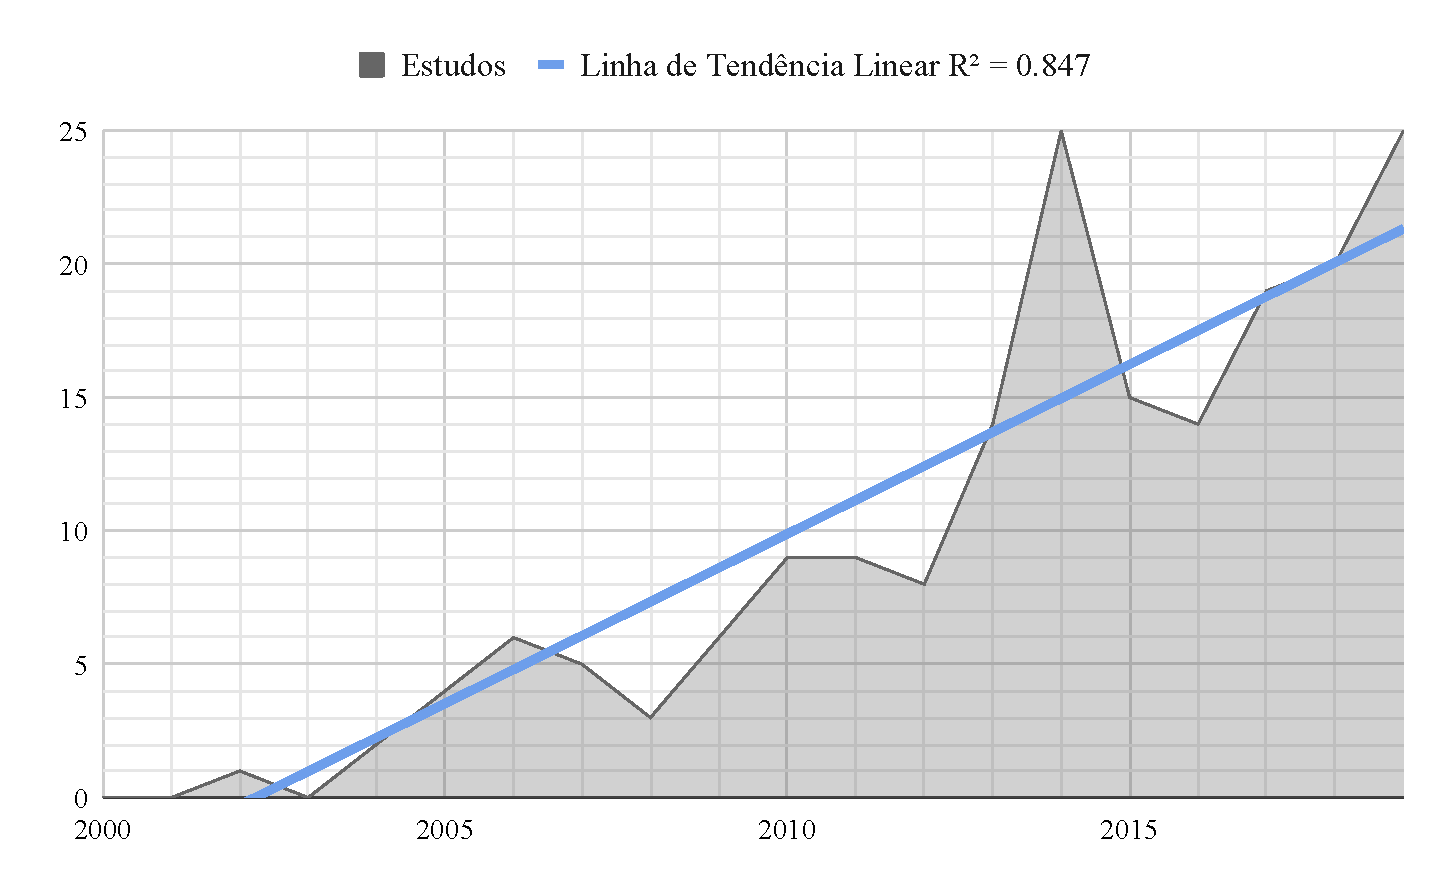
\includegraphics[width=\columnwidth]{images/publications-sm-timeline.pdf}}
\fautor
\end{figure}

%Outro dado relevante diz respeito às fontes das publicações, que também podem compor o racional das buscas manuais em possíveis estudos futuros. No contexto brasileiro, os 46 artigos classificados como relevantes na busca manual nacional podem ser avaliados sob essa perspectiva. Sendo assim, a Tabela \ref{results:table:manual-search-brazil} apresenta as conferências e periódicos destes estudos, que não foram considerados em nosso QGS porque as bases de dados, utilizadas nas buscas automatizadas, indexam predominantemente estudos em inglês. Considerando estes trabalhos, tem-se uma percepção mais assertiva com relação a Libras, tema onipresente nas publicações em questão.

%Por outro lado, a Tabela \ref{results:table:publication-venues} apresenta os principais locais de publicação, considerando os 139 estudos primários obtidos de fontes internacionais, os quais estão ordenados pela quantidade de estudos selecionados. Nesse contexto, a presença de conferências e periódicos definidos na busca manual internacional (em destaque na Tabela) sugere uma execução efetiva dessa fase considerando o protocolo de busca adotado.

Outro dado relevante diz respeito às fontes das publicações, que também podem compor o racional das buscas manuais em possíveis estudos futuros. A \autoref{results:table:publication-venues} apresenta os principais locais de publicação, considerando todos os estudos primários deste MS, os quais estão ordenados pela quantidade de estudos selecionados. No contexto internacional, a presença de conferências e periódicos definidos na busca manual (em destaque na Tabela) sugere uma execução efetiva dessa fase considerando o protocolo de busca adotado.

\begin{table}[htbp]
\caption{Conferências/Periódicos mais relevantes}
\label{results:table:publication-venues}
\centering
\begin{tabular}{lcc|lcc}
\hline
\multicolumn{3}{c|}{\textbf{Internacionais (\textit{INT})}} & \multicolumn{3}{c}{\textbf{Nacionais (\textit{BRA})}} \\ \hline
\textbf{Nome} & \textbf{Fonte} & \textbf{Estudos} & \textbf{Nome} & \textbf{Fonte} & \textbf{Estudos} \\ \hline
\textit{\textbf{HCI International}} & \textit{\textbf{Springer}} & \textit{\textbf{12}} & RENOTE & CINTED & 13 \\ 
ICCHP & Springer & 8 & SBIE & CEIE & 13 \\ 
\textit{\textbf{ICALT}} & \textit{\textbf{IEEE}} & \textit{\textbf{6}} & WCBIE & CEIE & 11 \\ 
ASSETS & ACM & 6 & WIE & CEIE & 7 \\ 
\textit{\textbf{Computers \& Education}} & \textit{\textbf{Elsevier}} & \textit{\textbf{5}} & RBIE & CEIE & 2 \\ 
Procedia Computer Science & Elsevier & 5 & - & - & - \\ 
Outros & - & 97 & - & - & - \\ 
\multicolumn{2}{l}{\textbf{Total}} & \textbf{139} & \multicolumn{2}{l}{\textbf{Total}} & \textbf{46} \\ \hline
\end{tabular}
\fautor
\end{table}

Além disso, foi analisada a distribuição dos estudos primários internacionais por país de origem. Nesse contexto, identificou-se uma grande quantidade de publicações relevantes nos Estados Unidos e Brasil, com 22 e 21 artigos respectivamente, que juntos representam 31\% dos estudos primários deste MS. Com isso, mesmo desconsiderando os estudos selecionados pela busca manual nas fontes nacionais, o Brasil se destacou internacionalmente na publicação de trabalhos que exploram o uso da tecnologia para o ensino e aprendizagem através das línguas de sinais.

Lembrando que as conferências e periódicos das buscas manuais foram definidos com o apoio de especialistas nas áreas de ES e educação. Para isso, critérios como relevância do evento e facilidade no acesso às publicações foram levados em consideração. Entretanto, tais critérios são subjetivos e, portanto, estão sujeitos a viés. Além disso, alguns dos locais sugeridos (internacional e nacionalmente) não identificaram nenhum estudo relevante. Portanto, possíveis replicações deste MS devem ponderar eventuais evoluções nos eventos definidos para as buscas manuais.

A seguir são discutidos os principais resultados deste trabalho, de modo a responder cada QP definida no escopo do MS. Adicionalmente, com o objetivo de organizar os estudos primários, eles serão classificados com relação à sua origem: internacional (\textit{INT}) ou nacional (\textit{BRA}). Com isso, os resultados podem ser isolados, o que pode beneficiar o planejamento e condução de trabalhos futuros.

\subsubsection{Soluções Tecnológicas (QP1)}

%A primeira questão de pesquisa tem como objetivo identificar os tópicos formais da ES que também vêm sendo investigados e adotados no cenário da educação por meio das línguas de sinais. As áreas identificadas foram classificadas com base na estrutura \textit{Software Engineering Body of Knowledge} (\textit{SWEBOK}) \cite{Bourque2014, Petersen2015}.

A primeira questão de pesquisa têm como objetivo identificar as vertentes de desenvolvimento exploradas para a construção de soluções educacionais com suporte a línguas de sinais. Para isso, as contribuições deste MS foram classificadas com base na estrutura \textit{Software Engineering Body of Knowledge} (\textit{SWEBOK}) \cite{Bourque2014, Petersen2015}.

Sendo assim, foram consideradas as quinze áreas possíveis da ES do \textit{SWEBOK}, das quais quatro foram exploradas pelos estudos primários deste MS. Essa concentração já era esperada, pois definimos como objetivo encontrar soluções tecnológicas em um domínio específico, o que geralmente remete a áreas mais técnicas. A \autoref{results:table:se-areas} apresenta as áreas da ES identificadas nesta pesquisa, considerando os 185 estudos primários (139 Internacionais e 46 Brasileiros).

\begin{table}[htbp]
\caption{Áreas da ES (SWEBOK)}
\label{results:table:se-areas}
\centering
\begin{tabular}{lcccc}
\hline
                          & \multicolumn{2}{c}{\textbf{\textit{INT}}} & \multicolumn{2}{c}{\textbf{\textit{BRA}}} \\ \cline{2-5} 
\textbf{Área da ES}       & \textbf{Estudos} & \textbf{\%}             & \textbf{Estudos} & \textbf{\%}             \\ \hline
Construção de Software    & 65               & 47\%                    & 23               & 50\%                    \\ 
Projeto de Software       & 47               & 34\%                    & 5                & 11\%                    \\ 
Fundamentos da Engenharia & 24               & 17\%                    & 9                & 19\%                    \\ 
Qualidade de Software     & 3                & 2\%                     & 9                & 19\%                    \\ 
\textbf{Total}            & \textbf{139}     & \textbf{100\%} & \textbf{46}      & \textbf{100\%} \\ \hline
\end{tabular}
\fautor
\end{table}

\begin{itemize}
    \item \textit{Construção de Software}: estudos com ênfase no desenvolvimento de soluções, incluindo seus respectivos detalhes de construção. Além disso, podem apresentar definições secundárias de design e qualidade. Por fim, o projeto e implementação de APIs (\textit{Application Programming Interfaces}) também são classificados nessa área;
    \item \textit{Projeto de Software}: estudos que apresentam conceitos de análise e projeto aplicados à soluções tecnológicas. Abstrações como arquiteturas e frameworks também são comuns nessa vertente;
    \item \textit{Fundamentos da Engenharia}: estudos com foco na avaliação empírica de suas soluções. Sendo assim, essa área possui relação direta com estudos de caso, surveys e experimentos.
    \item \textit{Qualidade de Software}: estudos com avaliações e validações não formais, relacionadas a critérios de qualidade minimamente estruturados. Revisões e auditorias de garantia de qualidade também são conduzidas nessa área.
\end{itemize}

Considerando as áreas da ES, é evidente que a maioria dos estudos primários apresentem o ``\textit{Projeto}'' e ``\textit{Construção}'' de soluções para o ensino/aprendizagem através das línguas de sinais. Por outro lado, existe uma quantidade importante de estudos com ênfase em avaliações empíricas, o que mostra a importância das avaliações formais na ES. Esses estudos foram classificados na área ``\textit{Fundamentos da Engenharia}'' (\textit{INT8, INT9, INT11, INT12, INT17, INT22, INT30, INT31, INT32, INT33, INT38, INT39, INT40, INT43, INT45, INT77, INT83, INT84, INT91, INT93, INT98, INT113, INT130, INT131, BRA14, BRA17, BRA22, BRA27, BRA28, BRA35, BRA37, BRA40, BRA46}).

É importante observar, ainda, que muitos outros artigos apresentavam avaliações empíricas, mas foram classificados em outras áreas da ES, semanticamente mais adequadas a suas respectivas contribuições primárias. Nesse cenário, 47.5\% dos estudos primários do MS apresentaram algum tipo de avaliação empírica -- \textit{survey}, estudo de caso ou experimento \cite{Wohlin2012}. Por outro lado, considerando a busca manual nacional, essa porcentagem foi ligeiramente superior, com um total de 52.1\%. Assim, é possível aferir que aproximadamente a metade dos estudos primários identificados possuem algum tipo de avaliação formal.

No entanto, existe um número inferior de estudos com ênfase em avaliações não empíricas, cujo principal objetivo geralmente é conduzir validações menos estruturadas em um determinado domínio de aplicação. Tais estudos foram classificados como ``\textit{Qualidade de Software}''. Nesse sentido, o MS retornou um número baixo de estudos com esta contribuição primária, cerca de 2\% (\textit{INT59, INT76, INT117}). Já a busca manual nacional obteve aproximadamente 19\% de seus estudos nesta categoria (\textit{BRA6, BRA7, BRA8, BRA9, BRA10, BRA11, BRA16, BRA18, BRA26}), evidenciando que esta é uma área da ES muito investigada no Brasil. 

De modo geral, as contribuições dos estudos primários foram classificadas em software, hardware ou teórica. Com isso, este trabalho identificou que 69.8\% de seus estudos têm ênfase em software, 11.3\% em hardware (\textit{INT11, INT12, INT19, INT43, INT58, INT61, INT65, INT67, INT71, INT88, INT97, INT102, INT105, INT108, INT125, INT133, INT137, INT138, BRA1, BRA14, BRA26}) e 18.9\% são contribuições teóricas (\textit{INT2, INT32, INT37, INT39, INT44, INT57, INT59, INT60, INT63, INT79, INT80, INT84, INT85, INT91, INT95, INT103, INT131, INT134, INT135, BRA6, BRA7, BRA8, BRA9, BRA10, BRA11, BRA13, BRA16, BRA17, BRA18, BRA22, BRA27, BRA28, BRA35, BRA37, BRA38}).

Desta forma, é possível concluir que a maioria das soluções tecnológicas para ensino e aprendizagem por meio de línguas de sinais vêm se baseando em software. Neste contexto, foram categorizados mais especificamente cada um dos estudos (\autoref{results:figure:publications-solutions}).

\begin{figure}[htbp]
\caption{Publicações por tipo de solução}
\label{results:figure:publications-solutions}
\centerline{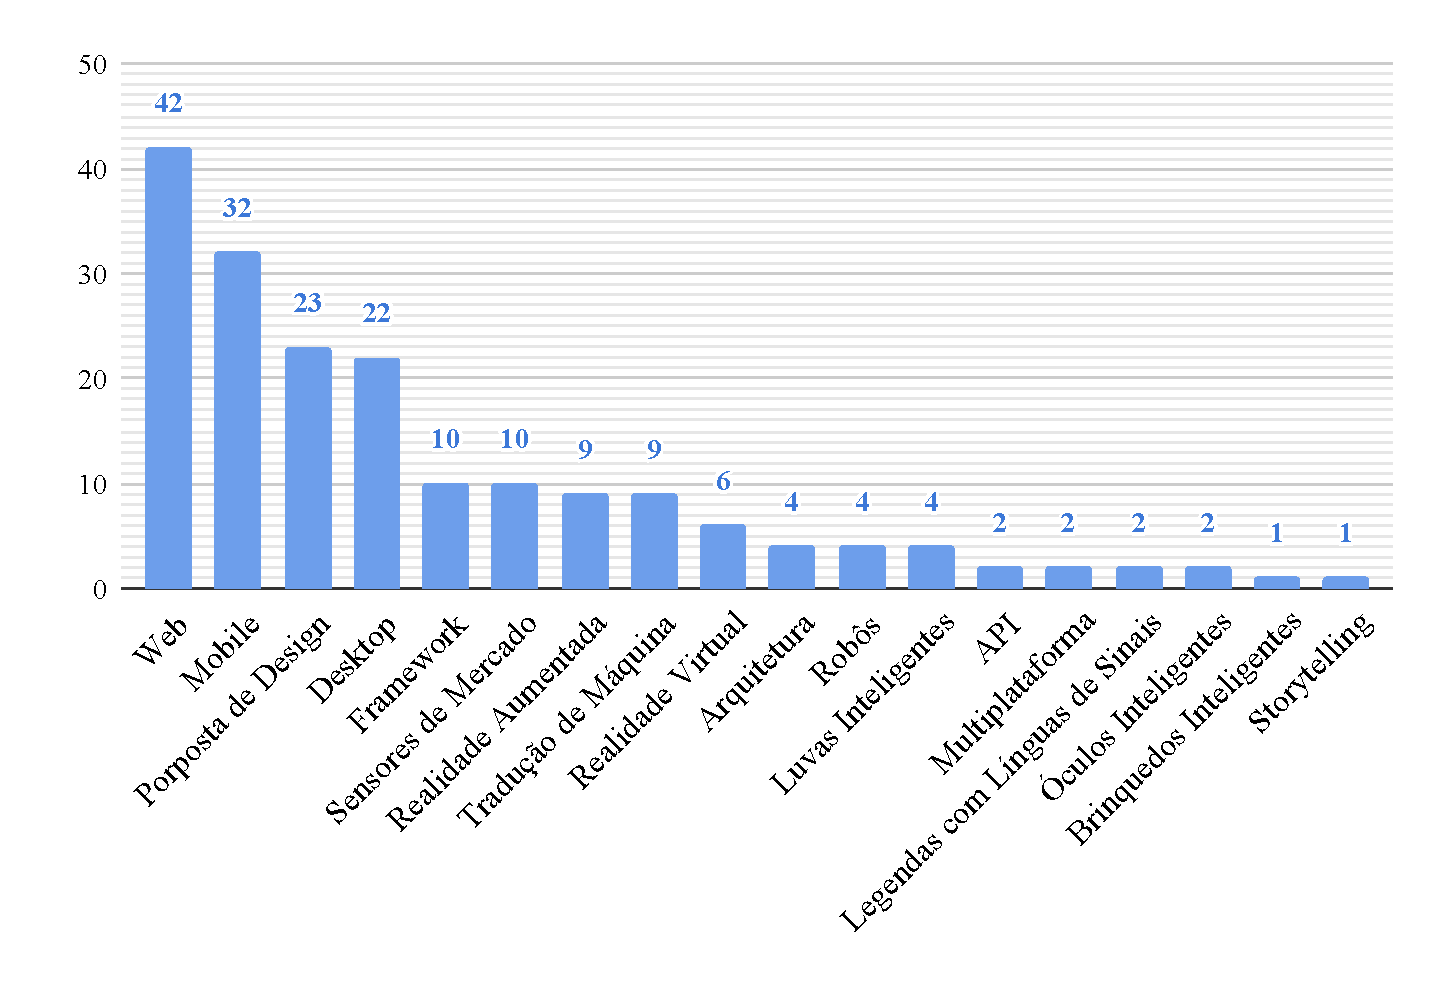
\includegraphics[width=\columnwidth]{images/publications-solutions.pdf}}
\fautor
\end{figure}

Essas informações evidenciam o dominância de algumas plataformas de desenvolvimento de software: Web, Mobile e Desktop. Juntas, essas plataformas equivalem a 52\% dos estudos primários. No entanto, foram identificadas apenas duas soluções que são claramente multiplataforma (\textit{INT70, INT116}). Essa pequena fração de contribuições pode denotar uma lacuna relevante em termos de usabilidade, já que a falta de uma experiência unificada pode prejudicar e/ou limitar a experiência dos usuários.

Sob outra perspectiva, diversas propostas de design foram identificadas (\textit{INT2, INT26, INT27, INT32, INT38, INT39, INT40, INT44, INT79, INT80, INT84, INT85, INT87, INT95, INT130, INT131, INT134, BRA13, BRA17, BRA30, BRA32, BRA37, BRA38}), mostrando que os potenciais projetos vêm sendo avaliados pela comunidade científica antes de sua efetiva implementação.

Propostas relacionadas à tradução de máquina e legendas de línguas de sinais foram classificadas individualmente (\textit{INT5, INT10, INT17, INT20, INT21, INT47, INT54, INT82, INT86, INT121, INT129}). Com isso, foi possível obter uma visão mais técnica sobre a complexidade e os desafios encontrados nesse tipo de solução, geralmente exploradas por meio de abordagens de Inteligência Artificial (IA). Nestas vertentes, não foram identificados artigos na busca manual nacional, porém três publicações do MS aplicam tais técnicas no contexto da Libras (\textit{INT17, INT20, INT47}). 

Uma quantidade significativa de estudos têm ênfase em sensores de mercado (\textit{INT19, INT43, INT58, INT61, INT97, INT105, INT108, INT138, INT123, BRA1}). Nesse sentido, os sensores Kinect\footnote{https://developer.microsoft.com/pt-br/windows/kinect}, Leap Motion\footnote{https://developer.leapmotion.com} e Myo Armband\footnote{https://developerblog.myo.com} foram os mais utilizados, nesta ordem. Isso evidencia que existem iniciativas na indústria que viabilizam o desenvolvimento de soluções para o reconhecimento de línguas de sinais por meio de hardware padronizados, comumente munidos de um Kit de Desenvolvimento de Software (SDK).

Por fim, os estudos primários demonstram que algumas técnicas e tecnologias vêm ganhando notoriedade. Nesse sentido, merece destaque o uso dos conceitos de Realidade Aumentada (RA) e Realidade Virtual (RV) em diversas soluções (\textit{INT34, INT46, INT69, INT77, INT96, INT106, INT124, INT135, BRA25, BRA29, BRA31}). Além disso, algumas API, frameworks e arquiteturas de software foram propostas (\textit{INT49, INT63, INT64, INT68, INT74, INT75, INT78, INT103, BRA22, BRA27, BRA28, BRA35, BRA44, BRA45}), mostrando que existem iniciativas para a criação de soluções mais genéricas e estruturadas nesse domínio.

\subsubsection{Tópicos Educacionais (QP2)}

A segunda QP identifica os tópicos educacionais das publicações, com o objetivo de entender melhor o público-alvo das soluções propostas. Para isso, foram extraídos os temas relacionados ao ensino e aprendizagem tendo em vista os estudos relevantes deste trabalho. A \autoref{results:table:educational-topics} sintetiza todos os tópicos educacionais identificados, considerando o MS e a busca manual nacional.

\begin{table}[htbp]
\caption{Tópicos Educacionais}
\label{results:table:educational-topics}
\centering
\begin{tabular}{lcccc}
\hline
                                 & \multicolumn{2}{c}{\textit{\textbf{INT}}} & \multicolumn{2}{c}{\textit{\textbf{BRA}}} \\ \cline{2-5} 
\textbf{Tópico Educacional}      & \textbf{Estudos}      & \textbf{\%}        & \textbf{Estudos}      & \textbf{\%}        \\ \hline
Línguas de Sinais                & 59                    & 42.4\%             & 19                    & 41.3\%             \\ 
Geral                            & 48                    & 34.5\%             & 10                    & 21.7\%             \\ 
Língua de Sinais Escrita         & 10                    & 7.2\%              & 3                     & 4.3\%              \\ 
Matemática                       & 7                     & 5.0\%              & -                     & -                  \\ 
Alfabeto                         & 6                     & 4.3\%              & 1                     & 2.2\%              \\ 
Ciência da Computação            & 4                     & 2.9\%              & 4                     & 8.7\%              \\ 
Língua Nativa do País            & 2                     & 1.4\%              & 9                     & 19.6\%             \\ 
Princípios Islâmicos             & 1                     & 0.7\%              & -                     & -                  \\ 
Ciências                         & 1                     & 0.7\%              & -                     & -                  \\ 
Aprendizagem Baseada no Trabalho & 1                     & 0.7\%              & -                     & -                  \\ 
\textbf{Total}                   & \textbf{139}          & \textbf{100\%}     & \textbf{46}           & \textbf{100\%}     \\ \hline
\end{tabular}
\fautor
\end{table}

Cerca de 42.2\% dos estudos investigam o ensino de línguas de sinais, evidenciando que ainda existem muitos desafios sendo investigados pela comunidade científica. Por outro lado, cerca de 31.3\% são estudos aplicados à educação, independentemente de um tópico; geralmente são soluções mais flexíveis e com uma capacidade disruptiva maior. Os outros 26.5\% estão distribuídos entre outros tópicos de ensino, nos quais destacam-se as línguas de sinais escritas, predominantemente baseadas em \textit{SignWriting}\footnote{http://signwriting.org} (\textit{INT9, INT25, INT26, INT27, INT28, INT29, INT30, INT31, INT64, INT68, BRA3, BRA19, BRA20}).

O \textit{SignWriting} é um sistema de escrita que usa símbolos visuais para representar as formas das mãos, movimentos e expressões faciais das línguas de sinais. Por meio dele é possível escrever qualquer sinal, independentemente da língua de sinais, sendo possível considerá-lo como um sistema de escrita universal. Entretanto, é preciso estudar seu alcance mundial e avaliar sua viabilidade prática.

Outra constatação interessante se dá pelo grande volume de estudos relacionados ao tópico de ensino e aprendizagem da língua nativa do país em que os usuários das línguas de sinais vivem (\textit{INT62, INT87, BRA5, BRA13, BRA15, BRA17, BRA21, BRA25, BRA26, BRA40, BRA41}). Particularmente, os trabalhos brasileiros se destacaram pelos esforços para o letramento bilíngue Português/Libras, evidenciando a busca pela educação inclusiva.

Ademais, identificou-se o publico-alvo dos estudos, com a intenção de complementar a resposta desta RQ. Assim, a maioria (aproximadamente 91.9\%) têm relação direta somente com usuários surdos. Isso evidencia que existem muitas iniciativas para inclusão da comunidade surda, nos mais diferentes contextos. Em contrapartida, apenas 8.1\% dos estudos têm um público-alvo mais abrangente, mas nem todos eles possuem iniciativa bilíngue.

Em particular, alguns desses estudos apresentam soluções que abrangem PcD intelectuais ou sensoriais adicionais (\textit{INT35, INT56, INT122, INT138}), enquanto outros investigam formas de reduzir as barreiras entre usuários e não usuários das línguas de sinais (\textit{BRA2, BRA7, BRA8, BRA10, BRA11, BRA12, BRA16, BRA18, BRA22, BRA27, BRA35}). Por conta disso, tais estudos tendem a investigar as línguas de sinais de maneira secundária, mas como uma ferramenta essencial de ensino e inclusão social.

\subsubsection{Línguas de Sinais (QP3)}

A última QP diz respeito ao uso das línguas de sinais no domínio educacional apoiadas pela tecnologia. Primeiramente foram identificadas as línguas de sinais mais pesquisadas pelos estudos primários, conforme a \autoref{results:table:sign-languages}. Novamente, EUA e Brasil estão no topo, com a \textit{American Sign Language} (ASL) e Libras. Essa é uma conclusão esperada, tendo em vista a distribuição dos estudos por país apresentada previamente.

\begin{table}[htbp]
\caption{Línguas de Sinais}
\label{results:table:sign-languages}
\centering
\begin{tabular}{lcccc}
\hline
           & \multicolumn{2}{c}{\textbf{\textit{INT}}} & \multicolumn{2}{c}{\textbf{\textit{BRA}}}  \\ \cline{2-5}

\textbf{Língua de Sinais} & \textbf{Estudos} & \textbf{\%}             & \textbf{Estudo} & \textbf{\%}               \\ \hline
ASL                       & 21               & 15.11\%                 & -               & -                         \\ 
Libras                    & 16               & 11.51\%                 & 44              & 95.65\%                   \\ 
Geral                     & 15               & 10.79\%                 & -               & -                         \\ 
SignWriting               & 10               & 7.19\%                  & 2               & 4.35\%                    \\ 
ArSL                      & 10               & 7.19\%                  & -               & -                         \\ 
PSL                       & 6                & 4.32\%                  & -               & -                         \\ 
BSL                       & 6                & 4.32\%                  & -               & -                         \\ 
MySL                      & 6                & 4.32\%                  & -               & -                         \\ 
ISL                       & 5                & 3.60\%                  & -               & -                         \\ 
Outras                    & 44               & 31.65\%                 & -               & -                         \\ 
\textbf{Total}            & \textbf{139}     & \textbf{100\%}          & \textbf{46}     & \textbf{100\%}            \\ \hline
\end{tabular}
\fautor
\end{table}

Analisando o histórico de publicações, a ASL apresentou contribuições relevantes desde 2004 (\textit{INT4, INT5, INT6, INT7, INT8, INT32, INT33, INT37, INT38, INT40, INT41, INT48, INT65, INT67, INT76, INT84, INT88, INT126, INT130, INT131, INT133}). Por outro lado, a Libras possui apenas seis estudos anteriores a 2010 (\textit{INT127, BRA3, BRA15, BRA26, BRA41, BRA42}), 10\% de um total de 60 estudos relevantes em Libras. Isso sugere um aumento expressivo nas publicações relacionadas à língua brasileira de sinais, em especial nos últimos dez anos. Sendo assim, o baixo índice de estudos relevantes anteriores a 2010 pode direcionar critérios de seleção em uma replicação ou estudo futuro.

Outras línguas de sinais merecem destaque, são elas: \textit{Arabic Sign Language} (ArSL), \textit{Portuguese Sign Language} (PSL), \textit{British Sign Language} (BSL), \textit{Malaysian Sign Language} (MySL) e \textit{Indian Sign Language} (ISL). Nesse contexto, soluções baseadas na ArSL vêm crescendo consistentemente nos últimos anos (\textit{INT1, INT10, INT13, INT14, INT15, INT16, INT21, INT58, INT66, INT136}).

Adicionalmente, alguns estudos foram classificados como ``Geral'' porque exploram o domínio de forma genérica/abstrata, mantendo a língua de sinais como um elemento secundário (\textit{INT19, INT22, INT39, INT44, INT46, INT59, INT63, INT71, INT79, INT85, INT106, INT114, INT122, INT124, INT138}). Entretanto, apenas um estudo enfatiza a possibilidade de uma unificação das línguas de sinais (INT79).

A \textit{SignWriting} aparece novamente com um número significativo de contribuições, mostrando que a língua de sinais escrita possui grande apelo cientifico (\textit{INT9, INT25, INT26, INT27, INT28, INT29, INT30, INT31, INT64, INT68, BRA3, BRA20}). Outros três estudos investigam múltiplas línguas de sinais (\textit{INT62, INT74, INT102}). Entretanto, nenhum deles apresenta uma solução genérica ou com alto nível de abstração para o desenvolvimento de soluções de escala global.

De modo geral, é possível concluir que existem muitas pesquisas relevantes no que tange ao domínio investigado neste MS. Ainda assim, a maioria das soluções são construídas sem o objetivo de compartilhar seus recursos (educacionais ou tecnológicos), o que dificulta o acesso à informação e a criação de soluções colaborativas. Nesse contexto, técnicas da ES podem ser efetivas para o desenvolvimento de estruturas genéricas com o objetivo de compartilhar tais recursos publicamente, visando a derivação de aplicações mais padronizadas no que tange ao domínio do ensino e aprendizagem através das línguas de sinais. Mais detalhes sobre tais possibilidades serão discutidos na proposta deste trabalho.

Por fim, as seções a seguir discutem alguns dos principais estudos primários, considerando os cenários internacional (\autoref{ms:cenario-internacional}) e nacional (\autoref{ms:cenario-nacional}) individualmente. Além disso, definições relevantes sobre o MS são retomadas, quando necessário, com o objetivo de contextualizar as análises e discussões em questão.

\section{Cenário Internacional}
\label{ms:cenario-internacional}

Inicialmente, considerando nosso protocolo de busca, identificamos algumas reflexões importantes relacionadas à condução deste MS. Primeiramente, a definição das bases para a busca manual foi conduzida cuidadosamente, isso porque os estudos selecionados nessa fase definiram o nosso principal critério de qualidade, o QGS. Nesse sentido, o apoio de especialistas foi essencial para a identificação de bases de dados relevantes, que tiveram sua importância aferida pela ocorrência representativa de estudos primários.

Posteriormente, durante a busca automatizada, concluímos que uma análise mais detalhada dos estudos do QGS pode ser extremamente efetiva na definição e refinamento da string de busca. Nesse contexto, a identificação de palavras chave e termos recorrentes fez com que nossos resultados incluíssem quase que totalmente os estudos do QGS, resultando em uma \textit{quasi-sensitivity} elevada.

Por sua vez, a abordagem de busca sistemática baseada em QGS foi essencial para a condução de um MS mais estruturado e formal. Com isso, decisões sensíveis como a definição das máquinas de busca ou a qualidade da string de busca puderam ser tomadas seguindo a diretriz de \citeonline{Zhang2011}. Sendo assim, os estudos primários (de fontes internacionais) discutidos neste trabalho foram identificados seguindo critérios de seleção sistemática rigorosos. Nesse contexto, selecionamos alguns desses 139 estudos com contribuições interessantes para essa discussão.

A  princípio, \citeonline{INT73} apresentaram um dos estudos mais completos desse MS, onde propõem uma ferramenta baseada em quiz para o aprendizado da Língua de Sinais Indiana (ISL). Inicialmente, os autores conduzem uma breve revisão de literatura, comparando a precisão da técnica proposta com outros métodos/aplicações. Em seguida eles propõem o design da solução, com ênfase no conceito de \textit{Automatic Sign Language Recognition} (ASLR). Por fim, a implementação e avaliação empírica são apresentadas, detalhando a arquitetura e mensurando a efetividade da solução experimentalmente.

\citeonline{INT47} e \citeonline{INT86}, propõem soluções de tradução de máquina baseadas em avatares 3D. Nesse sentido, considerando todos os 139 estudos primários obtidos em fontes internacionais, nós identificamos que soluções baseadas em avatares (3D ou 2D) equivalem a 26,6\% das contribuições selecionadas. Portanto, podemos deduzir que avatares representam parte significativa do estado da prática na representação das línguas de sinais.

\citeonline{INT47} apresentam um sistema baseado em corpus, essa categoria de soluções constrói conhecimento computacional a partir de exemplos ou modelos estatísticos. Nesse caso, o corpus foi construído a partir de um livro de ciências para crianças. Por fim, os detalhes arquiteturais e resultados de uma avaliação preliminar também são apresentados.

\citeonline{INT86} propõem uma solução para a geração automatizada de legendas em linguagem de sinais para vídeos. Nesse contexto, considerando o processo definido pelo sistema, caso um conjunto de sinais não seja reconhecido, um interprete de língua de sinais pode cadastrá-lo manualmente. Com isso, a base da dados é incrementalmente evoluída, aumentando assim a capacidade de tradução automática da solução interativamente.

Outro destaque são as soluções vestíveis, como luvas, óculos, relógios etc. Nesse âmbito, \citeonline{INT88} aplicaram o conceito de RA através de óculos inteligentes, com isso os PcD auditiva podem reunir todas as informações necessárias durante uma aula (instrutor, slides, intérprete de linguagem gestual ou legendas). Além disso, os autores conduziram um piloto e avaliaram a proposta experimentalmente.

Apenas um dos estudos primários explora explicitamente o conceito de API \cite{INT56}. Esse conceito representa um conjunto de rotinas e padrões disponíveis através de uma interface, para que outras aplicações possam consumir os recursos compartilhados de um domínio. Por esse motivo, APIs podem proporcionar a integração entre sistemas que possuem linguagem distintas de maneira ágil e segura, algo extremamente necessário para o desenvolvimento de uma solução educacional mais flexível e global. Sendo assim, \citeonline{INT56} propõem a \textit{Blind/Deaf Communications API} (BDC-API), um framework que traduz o conteúdo educacional digital para surdos e cegos. Os autores também propõem um modelo educacional baseado em \textit{Massive and Open Online Courses} (MOOCs) e apresentam detalhes do design da solução.

Muitos dos estudos selecionados exploram o conceito de gamificação, principalmente os destinados ao público infantil. Nesse sentido, \citeonline{INT109} apresentam o design, construção e avaliação empírica de um jogo educativo para ensinar números em Libras. Além disso, algo muito positivo é o fato do experimento em questão avaliar os recursos educacionais disponíveis no jogo.

Um estudo que nos chamou a atenção pela capacidade de adequação ao contexto de seus usuários foi o de \citeonline{INT53}. Os autores apresentam uma solução desktop relativamente simples, embarcada em DVD para o ensino da Língua de Sinais Australiana (Auslan). Entretanto, a aplicação possui uma funcionalidade interessante que possibilita a configuração da região do usuário. Isso é muito positivo e relevante porque em países com muita diversidade, é muito comum existirem variações regionais das línguas de sinais.

Por fim, \citeonline{INT79} é o nosso último estudo para discussão. Nele os autores discorrem sobre a dificuldade dos usuários das línguas de sinais em se comunicar de maneira global. Nesse contexto, os autores apresentam uma proposta inicial de trabalho e metodologia. Entretanto, sua contribuição principal é teórica, com o objetivo de refletirmos sobre a forma como as soluções atuais vem sendo desenvolvidas (na maioria das vezes focadas em uma língua de sinais específica).

De modo geral, apresentamos uma diversidade relevante de soluções neste MS. Através delas, identificamos o uso massivo das TICs e de técnicas de Inteligência Artificial (IA), principalmente nas subáreas das Redes Neurais, Visão Computacional e Aprendizado de Máquina. Desta forma, podemos concluir que nossas capacidades de hardware e software nunca foram tão elevadas,  possibilitando a criação de aplicações mais robustas e eficientes.

Por outro lado, não existem muitas propostas preocupadas em estruturar computacionalmente soluções educacionais voltadas às línguas de sinais. Sendo assim, acreditamos que técnicas da ES podem ajudar na proposição de aplicações educacionais que possuam uma arquitetura genérica e colaborativa, visando soluções globais de ensino e aprendizagem baseadas em línguas de sinais.

\section{Cenário Nacional (Libras)}
\label{ms:cenario-nacional}

%region [FalvoJr] Somente Estudos da Busca Manual Nacional

Considerando os estudos primários obtidos em âmbito nacional, 46 publicações foram selecionadas manualmente, as quais foram omitidas a priori por questões técnicas relacionadas ao QGS. Posteriormente, através da inclusão dessas contribuições para a extração dos resultados, foi possível obter uma visão estendida sobre o uso da tecnologia como ferramenta para o ensino/aprendizagem através da Libras. Desta forma, gostaríamos de estender os resultados supracitados, com uma atenção especial à Libras, um dos principais objetos de interesse desta pesquisa.

Com base nos resultados apresentados, é possível concluir que a Libras, no domínio educacional, vem sendo consistentemente apoiada por soluções tecnológicas diversas. Sendo assim, estudos nos quais a Libras é a língua de sinais primária somam 44 publicações, das 46 obtidas por meio da busca manual nacional. Alguns desses estudos primários são discutidos a seguir com a intenção de enriquecer os resultados apresentados com as principais contribuições nacionais.

Soluções baseadas em avatares 3D/2D equivalem a 19,6\% dos estudos primários nacionais, demostrando que essa é uma tendência nos âmbitos nacional e internacional. Em particular, no Brasil boa parte dos estudos investigou a efetividade desse tipo de solução, principalmente por meio da comparação entre aplicativos educacionais móveis (\textit{BRA6, BRA7, BRA8, BRA10, BRA11, BRA16, BRA18}). Dentre os mais avaliados estão: \textit{Hand Talk}\footnote{\url{https://handtalk.me}}; \textit{ProDeaf} (descontinuado, devido a ``fusão'' com o \textit{Hand Talk}); \textit{VLibras}\footnote{\url{https://vlibras.gov.br}}; e \textit{Rybená}\footnote{\url{https://portal.rybena.com.br/site-rybena}}. Considerando as evidências apresentadas, o \textit{Hand Talk} se mostrou a frente dos concorrentes, saindo-se melhor na interpretação, tradução e eventuais desambiguações.

Em uma perspectiva mais ampla, \citeonline{BRA12} apresentam uma plataforma educacional intitulada \textit{SalaBil}, com ênfase na educação bilíngue (Português e Libras). O principal objetivo da solução é auxiliar o professor na criação de materiais didáticos para uso com alunos surdos, a mesma é composta por uma área onde o tutor planeja e monta suas aulas e uma área onde o aluno realiza as atividades propostas, que podem ser: textos, imagens, jogos de memória, jogos de ligar e questionários. Os diferenciais da plataforma são um dicionário e o compartilhamento/reutilização de materiais didáticos.

Vários estudos nacionais exploram o conceito de gamificação em suas soluções, os quais têm como público alvo recorrente crianças surdas, geralmente em processo de alfabetização. Nesse sentido, \cite{BRA23} descrevem um jogo desenvolvido para instigar o pensamento lógico, chamado \textit{LibrasBot}, idealizado para ser um Recurso Educacional Aberto (REA) multidisciplinar. Por outro lado, \citeonline{BRA31} apresentam o aplicativo \textit{LibrAR} que implementa os conceitos de RA/RV para auxiliar no ensino das letras e números em Libras. Por fim, \citeonline{BRA39} apresentam o projeto e construção do jogo \textit{Gestus}, que tem por objetivo ensinar Libras para crianças de forma lúdica. Dentre os jogos identificados, o \textit{Gestus} é um dos que possui a interface visual mais elaborada e amigável.

Finalmente, algumas publicações contribuíram na vertente teórica por meio do conceito de Arquiteturas Pedagógicas (AP). Segundo \citeonline{BRA22}, uma AP pode ser definida pelo seguinte conjunto dos componentes: (i) objetivo de aprendizagem -- o que aprender; (ii) atividades -- o que fazer; (iii) método -- como desenvolver as atividades; e (vi) recursos digitais -- com quais ferramentas. Em outras palavras, são estruturas de aprendizagem compostas pela abordagem pedagógica, software, Internet, IA, Educação a Distância (EAD) e concepção de tempo e espaço \cite{BRA27}.

De modo geral, as TICs também tiveram destaque nas soluções identificadas nacionalmente, as quais exploram inúmeras tecnologias no domínio da educação inclusiva. Além disso, também foram apresentadas técnicas pedagógicas e abordagens de desenvolvimento bastante interessantes. Por outro lado, poucos estudos contribuíram no sentido de disponibilizar um arcabouço público visando a construção canônica e colaborativa de soluções educacionais voltadas às línguas de sinais. Sendo assim, acredita-se que padrões de projeto e implementação possam apoiar a proposição de aplicações educacionais com uma arquitetura genérica, tendo em vista soluções mais flexíveis de ensino e aprendizagem para os surdos.

%endregion [FalvoJr] Somente Estudos da Busca Manual Nacional

%region [FalvoJr] Todos os Estudos que Exploram a Libras

%Adicionalmente, os estudos primários foram estendidos com outros 46 publicações obtidas por meio da busca manual nacional. %, omitida a priori por questões técnicas relacionadas ao QGS. [falar que ela não foi considerada em um trabalho anterior, citando o artigo do FIE (se nao for blind)]
%Dessa forma, foi possível obter uma visão geral sobre o uso da tecnologia como ferramenta para o ensino/aprendizagem da Libras. Para isso, os estudos primários identificados pelo MS foram mesclados com os estudos classificados como relevantes durante busca manual nacional. Dito isso, serão discutir os resultados supracitados, mas com especial atenção em Libras, o objeto de interesse central desta pesquisa.

%Com base nos resultados apresentados, é possível afirmar que a Libras, no domínio educacional, vem sendo consistentemente investigada em algumas das principais áreas da ES. Sendo assim, estudos cuja Libras é a língua de sinais primária somam 60 publicações (16 de fontes internacionais e 44 selecionados pela busca manual nacional). Alguns desses estudos primários serão discutidos a seguir com a intenção de apresentar suas principais contribuições.

%\citeonline{INT47} propõem uma solução de tradução de máquina baseadas em avatares 3D. Nesse sentido, as soluções baseadas em avatares equivalem a 21.67\% das contribuições que exploram a Libras (\textit{INT17, INT34, INT47, INT80, BRA6, BRA7, BRA8, BRA10, BRA11, BRA16, BRA18, BRA29, BRA33}). Portanto, é possível inferir que avatares 3D representam parte significativa do estado da prática na representação das línguas de sinais. Adicionalmente, \citeonline{INT47} apresentam um sistema baseado em corpus\footnote{Categoria de soluções que constrói conhecimento computacional a partir de exemplos ou modelos estatísticos.}~. Nesse caso, o corpus foi criado a partir de um livro de ciências para crianças. Por fim, os detalhes arquiteturais e resultados de uma avaliação preliminar também são apresentados.

%Refinando o assunto de avatares 3D, uma parte dos estudos investiga a efetividade desse tipo de solução, principalmente por meio da comparação de aplicativos educacionais móveis (\textit{BRA6, BRA7, BRA8, BRA10, BRA11, BRA16, BRA18}). Dentre os software mais avaliados estão \textit{Hand Talk}\footnote{https://www.handtalk.me}~, \textit{ProDeaf} (descontinuado, devido à ``fusão'' com o \textit{Hand Talk}), \textit{VLibras}\footnote{https://www.vlibras.gov.br}~ e \textit{Rybená}\footnote{https://portal.rybena.com.br/site-rybena}~. Dentre os resultados apresentados, o \textit{Hand Talk} se mostrou a frente dos concorrentes, saindo-se melhor na interpretação, tradução e eventuais desambiguações.

%Vários estudos selecionados investigam conceitos de gamificação em suas soluções educacionais (\textit{INT92, INT109, BRA2, BRA12, BRA23, BRA24, BRA25, BRA31, BRA34, BRA36, BRA37, BRA39}), principalmente os destinados ao público infantil. Nesse sentido, \citeonline{BRA23} descrevem o desenvolvimento de um jogo chamado \textit{LibrasBot}, desenvolvido para ser um Recurso Educacional Aberto (REA) multidisciplinar. O principal objetivo é fomentar o ensino da robótica e desenvolver o aprendizado de Libras.

%Ainda na categoria de jogos, \citeonline{BRA31} apresentam o aplicativo \textit{LibrAR} que implementa os conceitos de RA/RV para auxiliar no ensino das letras e números em Libras. A solução possui três módulos: o primeiro apresenta uma mão 3D para ensinar os sinais; o segundo e o terceiro são jogos para que o usuário treine seus conhecimentos em Libras, com possibilidade de imersão por meio de RA (\textit{smarthphones}) ou RV (\textit{cardboards}).

%\citeonline{BRA39} apresentam o projeto e construção do jogo \textit{Gestus}, que tem por objetivo ensinar Libras para crianças de forma lúdica. Seu desenvolvimento foi baseado na metodologia \textit{Design Thinking} e consiste em um conjunto de mini \textit{games} que ensinam palavras e expressões em Libras, visando auxiliar as crianças surdas no complexo processo de inclusão social no contexto escolar. Dentre os jogos apresentados, este é o que possui a interface visual mais elaborada e amigável.

%Finalmente, algumas publicações contribuíram na vertente teórica apresentando o conceito de Arquiteturas Pedagógicas (APs) (\textit{BRA22, BRA27, BRA35}). Segundo \citeonline{BRA22}, uma AP pode ser definida pelo seguinte conjunto dos componentes: (i) objetivo de aprendizagem -- o que aprender; (ii) atividades -- o que fazer; (iii) método -- como desenvolver as atividades; e (vi) recursos digitais -- com quais ferramentas. Em outras palavras, são estruturas de aprendizagem compostas pela abordagem pedagógica, software, Internet, IA, Educação a Distância (EaD) e concepção de tempo e espaço \cite{BRA27}.

%endregion [FalvoJr] Todos os Estudos que Exploram a Libras

\section{Considerações finais}
\label{ms:fim}

Nesta seção, foi apresentada uma visão geral das pesquisas realizadas sobre o uso da tecnologia para o ensino e aprendizagem através das línguas de sinais. Um MS baseado no conceito de QGS foi conduzido, resultando em 139 estudos selecionados \cite{FalvoJr2020_FIE}. Adicionalmente, a busca manual nacional foi utilizada como uma extensão dos estudos primários do MS, incluindo mais 46 publicações \cite{FalvoJr2020_SBIE}. Com isso, os artigos foram classificados de acordo com suas soluções tecnológicas, tópicos educacionais e línguas de sinais para responder as QP definidas. 

Alguns dos principais estudos primários selecionados também foram discutidos, abordando temas como o nível de abstração e capacidade de escala global das soluções nos âmbitos nacional e internacional. Mais detalhes sobre os estudos primários discutidos podem ser encontradas no \autoref{apendice:estudos-primarios}, que tabula todas as contribuições abordadas nas Seções \ref{ms:cenario-internacional} e \ref{ms:cenario-nacional}. Além disso, lembramos que o acesso aos estudos primários na íntegra e seus respectivos dados extraídos estão disponíveis pelo link: \url{https://bit.ly/SM-DataExtraction}.

Resumidamente, identificou-se que a maioria das soluções dizem respeito ao design ou construção de software. De forma adicional, metade dos estudos primários apresentam alguma avaliação empírica, o que evidencia a importância de um processo de avaliação formal. Em aspectos técnicos, as soluções estão divididas entre as plataformas Web, Mobile e Desktop, mas alguns estudos enfatizam abordagens/tecnologias mais específicas como tradução de máquina, sensores, RA/RV, frameworks, arquiteturas etc.

Sobre os tópicos educacionais, existe uma grande incidência de soluções para o ensino de línguas de sinais, um resultado esperado considerando os termos utilizados na nossa string de busca. De forma complementar, uma língua de sinais escrita merece destaque, chamada \textit{SignWriting}. Através dela é possível se comunicar  independentemente da língua de sinais nacional, pois cada usuário interpretará o sinal em sua língua nativa. Tal característica viabiliza uma série de possibilidades para a criação de soluções de âmbito global. Entretanto, uma pesquisa mais aprofundada deve ser conduzida para uma discussão mais fundamentada.

Finalmente, considerando as línguas de sinais, identificamos uma predominância da ASL e da Libras. Adicionalmente, muitas outras línguas de sinais foram mapeadas, inclusive a \textit{SignWriting}. Além disso, alguns estudos tratam as línguas de sinais de forma genérica. Entretanto, nenhum deles apresentou uma implementação concreta visando a unificação ou coexistência das línguas de sinais, o que poderia derivar um interessante tópico de pesquisa.

Este MS apresenta algumas ameaças à validade relevantes que devem ser ponderadas em possíveis trabalhos futuros, como replicações e/ou atualizações deste MS. Nesse sentido, os principais pontos de atenção identificados durante o processo descrito neste trabalho foram mapeados e estão disponíveis a seguir:

\begin{itemize}
\item Primeiramente,  é importante ressaltar que o primeiro autor realizou individualmente todas as etapas deste MS, incluindo a seleção dos estudos (buscas manual e automatizada), leitura, classificação e extração de dados. Todavia, os coautores forneceram \textit{feedback} contínuo sobre todas as etapas, com o objetivo de minimizar esse viés; 
\item Considerando o protocolo do MS, este estudo limitou o período de publicação dos trabalhos selecionados entre 2000 e 2019, pois acredita-se que contribuições anteriores não representariam as abordagens educacionais atuais, especialmente considerando o contexto da ES \cite{Radermacher2013,Scatalon2019}. Não obstante, a pouca incidência de publicações nos anos iniciais desse período pode representar um critério de seleção coerente.
\item Por fim, o uso da abordagem de busca sistemática baseada em QGS não garante a qualidade dos estudos selecionados. Entretanto, outras diretrizes consolidadas da ES também foram utilizadas, com o objetivo minimizar vieses nos resultados deste estudo.
\end{itemize}

%Como trabalhos futuros, pretende-se consolidar os aspectos estruturais e técnicos analisados nesta seção para proposição de uma abstração de software formal, com o objetivo de reduzir a complexidade na criação de aplicações educacionais baseadas em línguas de sinais. Nesse contexto, a \autoref{chapter:proposta} apresenta uma proposta de projeto fortemente pautada pelos resultados apresentados neste MS.
Como trabalhos futuros, a partir do MS conduzido observou-se que poucos estudos contribuíram no sentido de disponibilizar um arcabouço público visando o desenvolvimento colaborativo de soluções educacionais voltadas às línguas de sinais. Nesse sentido, acredita-se que conceitos da ES podem reduzir a complexidade para a criação de aplicações educacionais através de uma abstração de software formal, tendo em vista soluções padronizadas de ensino e aprendizagem baseadas em línguas de sinais. Nesse contexto, a \autoref{chapter:proposta} apresenta uma proposta de projeto fortemente pautada pelos resultados apresentados neste MS.
\chapter{Proposta de Trabalho}
\label{chapter:proposta}

\section{Caracterização da pesquisa}

Atualmente, temas relacionados ao ensino e aprendizagem têm sido cada vez mais discutidos e estudados pela comunidade científica. Em especial, ambientes computacionais de aprendizagem têm apresentando uma crescente importância, desempenhando um papel fundamental em atividades de ensino e treinamento, sendo relevantes não apenas no âmbito acadêmico como também no que se refere a inclusão social/digital de pessoas com necessidades especiais no mundo todo \cite{Svetlana2009,Bersch2017,Cilli2017}.

Em uma perspectiva relacionada, o advento da tecnologia vem impactando positivamente as dinâmicas de ensino e aprendizagem. Particularmente, a união entre as TICs e práticas pedagógicas modernas tem proporcionado ambientes educacionais mais dinâmicos e inclusivos \cite{Cilli2017}. Nesse contexto, este trabalho tem como principal objetivo propor uma infraestrutura que auxilie na criação de aplicações educacionais inclusivas com suporte a línguas de sinais e educação bilíngue.

Para isso, refletir sobre os estudos primários obtidos no MS deste trabalho foi fundamental. De modo geral, a maioria das soluções identificadas conduziu a fase de desenvolvimento do software sem seguir padrões/técnicas de reuso da ES. Isso resultou em aplicações monolíticas geralmente focadas em um domínio de ensino e aprendizagem específico, prejudicando assim o compartilhamento de seus recursos educacionais e criando soluções acessíveis, mas não inclusivas.

Em contrapartida, algumas contribuições exploram conceitos mais interessantes do ponto de vista técnico, os quais possibilitam o compartilhamento ordenado de recursos educacionais e/ou tecnológicos. Nesse sentido, os seguintes conceitos foram identificados como potenciais abstrações para esta proposta de trabalho:

\begin{itemize}
    \item \textit{Arquitetura}: pode ser definida como uma estrutura ou organização lógica de componentes, com suas respectivas interações e estrutura da informação \cite{Pressman2016}. %Entretanto, existem inúmeras variações deste termo, as quais podem alterar seu nível de abstração e domínio de aplicação, como por exemplo a Arquitetura de Referência ou Arquitetura Pedagógica;
    \item \textit{Framework}: abstração que une códigos comuns entre vários projetos de software com características similares, provendo configurações e componentes genéricos \cite{Sommerville2015}.
\end{itemize}

Por definição, frameworks são menos abstratos que arquiteturas, pois possuem implementações concretas dentro de si. Portanto, entende-se que uma arquitetura seja mais adequada ao contexto deste projeto. Desta forma, as aplicações educacionais poderão ser desenvolvidas com mais liberdade em termos de implementação, desde que a arquitetura proposta seja respeitada. Em particular, optou-se pela Arquitetura Orientada a Serviços (SOA -- \textit{Service-Oriented Architecture}), principalmente pela sua flexibilidade e consonância com as infraestruturas em nuvem atuais.

Através de uma arquitetura SOA, é possível construir uma API genérica voltada ao domínio das aplicações educacionais com suporte as línguas de sinais. Lembrando que APIs são uma das formas mais utilizadas pela indústria para o compartilhamento de recursos, pois elas podem expor interfaces de software totalmente personalizáveis em termos de acesso à informação, permitindo assim integrações seguras e gerenciáveis. Nesse contexto, o estilo arquitetural \textit{\textbf{RE}presentational \textbf{S}tate \textbf{T}ranfer} (REST) merece destaque, principalmente devido a sua total sinergia com o protocolo \textit{HyperText Transfer Protocol} (HTTP) \cite{Fielding2000}, o precursor da Web moderna.

Adicionalmente, o conceito de REA, apesar de identificado em apenas um estudo no MS \cite{BRA23}, é considerado intrínseco nesta proposta, principalmente tendo em vista a criação da API de forma pública e colaborativa para prover recursos de ensino/aprendizagem baseados em línguas de sinais. Com isso, a abstração de software idealizada para este projeto é uma arquitetura SOA baseada no estilo arquitetural REST, a qual será desenvolvida e disponibilizada como um software livre, respeitando as premissas dos REAs. %Entretanto, esta decisão ainda será avaliada, considerando especialistas na área da ES.

De modo geral, o objetivo principal deste projeto de doutorado é prover uma infraestrutura que permita a criação de aplicações educacionais no contexto do ensino bilíngue, de forma simples e padronizada. Para isso, uma API será desenvolvida e implantada para abstrair grande parte da complexidade desse domínio de aplicação. Dessa forma, inúmeras soluções poderão ser instanciadas a partir dessa arquitetura central, as quais poderão explorar os tópicos educacionais pertinentes/permitidos aos seus respectivos contextos.

Por exemplo, considerando o \textit{Hand Talk}, um dos aplicativos de Libras com maior destaque em âmbito nacional, tem-se algumas funcionalidades interessantes pensando no desenvolvimento de soluções baseadas na infraestrutura proposta (\autoref{proposal:handtalk}): (a) tradução de texto e áudio para Libras, a qual é interpretada por um avatar 3D. De modo adicional, o usuário também pode optar por mudar a língua de sinais para a ASL; (b) dicionário categorizado com a representação das palavras em sinais (disponível apenas para a Libras); e (c) vídeos educacionais  (disponíveis apenas para a Libras) abordando tópicos de interesse dos usuários do aplicativo.

\begin{figure}[htbp]
\centering
\caption{Aplicativo \textit{Hand Talk}}
\label{proposal:handtalk}
\begin{tabular}{ccc}
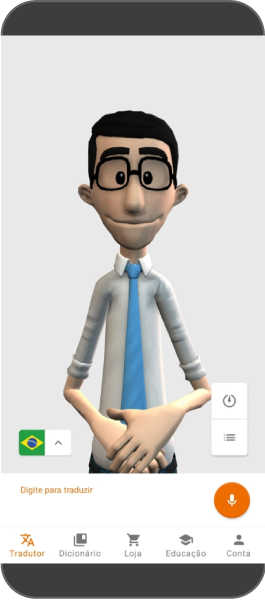
\includegraphics[width=0.275\textwidth]{images/handtalk-01.png} & 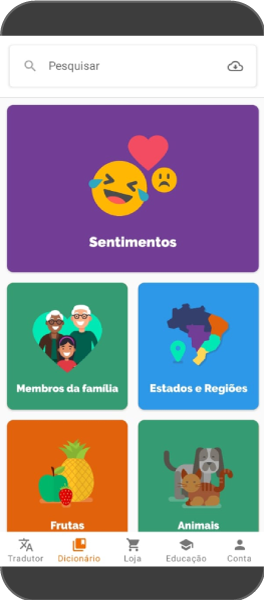
\includegraphics[width=0.275\textwidth]{images/handtalk-02.png} & 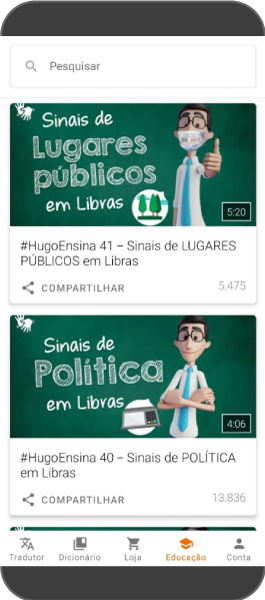
\includegraphics[width=0.275\textwidth]{images/handtalk-03.png}\\
(a) Tradutor & (b) Dicionário & (c) Educação (Vídeos) \\
\end{tabular}
\caption*{Fonte: \url{www.handtalk.me}.}
\end{figure}

Nesse contexto, entende-se que a gama de soluções no domínio educacional é extensa. Sendo assim, para a criação de uma solução baseada na infraestrutura proposta, optou-se por um tópico de ensino comum e fundamental a ambas línguas (Libras e Português), a Matemática. Consequentemente, uma solução bilíngue é desenhada, com a qual falantes e sinalizantes podem interagir através de uma experiência inclusiva. Em termos técnicos, optou-se por uma aplicação educacional móvel, tendo em vista a grande relevância desses dispositivos apresentada nas Seções \ref{chapter:fundamentacao-teorica} e \ref{chapter:mapeamento-sistematico} deste trabalho. Por outro lado, arquiteturalmente, a API é a responsável pela maior parte do esforço computacional da infraestrutura em questão. A seguir, algumas das tarefas de desenvolvimento planejadas são descritas:  %algumas dessas possibilidades estão sendo analisadas quanto a viabilidade de implementação, são elas:

\begin{itemize}
    \item Tradução de máquina: para que seja possível a tradução bidirecional (texto/voz para língua de sinais e língua de sinais para texto/voz) técnicas de IA serão exploradas, principalmente tendo vista algoritmos relacionados a visão computacional (``ler'' os sinais) e redes neurais (tradução);
    \item Internacionalização (I18n) e Localização (L10n): explorando recursos de geolocalização, espera-se que as soluções instanciadas sejam sensíveis ao contexto de seus usuários. Podendo com isso, adaptar-se a uma variação regional de uma das línguas, quando necessário. Além disso, essa estrutura pode viabilizar a tradução entre línguas de sinais, possibilitando a comunicação entre uma pessoa fluente em ASL e outra em Libras, por exemplo;
    \item Criação de conteúdo educacional: uma estratégia colaborativa é idealizada, na qual usuários fluentes (muitas vezes professores) criam as atividades em um painel administrativo. Com isso, seus respectivos alunos são notificados sobre esses novos desafios. Consequentemente, uma base de dados extremamente rica é criada, a qual, com o tempo, proverá recursos educacionais cada vez mais efetivos e adequados ao contexto de seus aprendizes. Além disso, como a infraestrutura idealizada é genérica com relação às línguas de sinais, línguas menos evidentes (como as locais e rurais) também podem ser exploradas, mantendo assim seu legado linguístico. %aqui temos uma série de alternativas, dentre as mais interessantes estão a criação de recursos para o ensino de línguas de sinais ou, visando uma validação inicial, o alfabeto. Além disso, o conceito de gamificação se mostrou bastante presente nos estudos primários, indicando uma linha de pesquisa em evidência.
\end{itemize}

\section{Atividades e cronograma}

Tendo em vista os objetivos pretendidos, esta seção define o plano de trabalho e o cronograma idealizados para a condução das tarefas deste projeto de doutorado. Nesse sentido, uma síntese das principais atividades a serem executadas é apresentada a seguir:

\begin{enumerate}
    \item [A.]\textbf{Levantamento e estudo sobre línguas de sinais e TICs na educação:} esta atividade consiste na investigação de referenciais teóricos para identificação dos principais conceitos e limitações relacionados ao ensino e aprendizagem em dois domínios específicos: (i) línguas de sinais; e (ii) TICs. Sendo assim, os temas inclusão digital e educação inclusiva possuem grande relevância para a criação de ambientes de ensino cada vez mais acessíveis em todos os aspectos;
    
    \item [B.]\textbf{Mapeamento Sistemático sobre tecnologia, educação e línguas de sinais:} visa realizar uma busca sistemática e abrangente com a intenção de selecionar estudos relevantes para extração e análise de informações pertinentes às questões de pesquisa estabelecidas. Com isso, espera-se obter uma visão geral sobre o estado da prática com relação ao uso da tecnologia como ferramenta de apoio na educação baseada em línguas de sinais;
    
    \item [C.]\textbf{Proposição de uma arquitetura SOA para a criação de aplicações educacionais baseadas em línguas de sinais:} a partir dos estudos identificados pelas atividades A e B, esta tarefa consiste em projetar a arquitetura em questão para a validação da mesma.%o desenvolvimento de aplicações com arquitetura e recursos educacionais compartilhados. Desta forma, a solução se beneficia exponencialmente do reuso e colaboração de suas instâncias, criando uma base de conhecimento cada vez mais rica e eficiente em resolver seus problemas de negócio;
    
    \item [D.]\textbf{Avaliação da arquitetura por meio de entrevistas e/ou questionários com especialistas:} esta atividade tem como objetivo avaliar a abstração apresentada através do feedback de especialistas nos domínios da ES, educação e, se possível, línguas de sinais;
    
    \item [E.]\textbf{Refinamento da arquitetura proposta:} a partir das limitações e problemas identificados na atividade anterior, a arquitetura proposta pode ser refinada/evoluída antes de tornar-se um infraestrutura em nuvem. Portanto, quaisquer artefatos e/ou estruturas devem ser devidamente revisados não apenas com viés técnico, mas também nos âmbitos da educação e línguas de sinais;
    
    \item [F.]\textbf{Criação de uma aplicação educacional móvel para o ensino bilíngue de Matemática:} esta atividade consiste no desenvolvimento de uma solução, tendo em vista a infraestrutura disponível. Proposta de modo a gerar uma aplicação educacional móvel com suporte a multilínguas, explorando os conceitos de internacionalização (i18n) e localização (l10n). Mais especificamente, se espera criar uma solução bilíngue, a qual sirva como TA no processo de educação inclusiva;
    
    \item [G.]\textbf{Avaliação da aplicação:} tem como objetivo avaliar o produto criado, por meio da condução de experimentos seguindo as recomendações da engenharia de software experimental. Nesse sentido, a aplicação educacional móvel será avaliada experimentalmente a partir de sua utilização em ambientes reais de ensino e aprendizagem. Para isso, a princípio existem duas alternativas: (i) comparar os resultados dos participantes com um grupo que não utilizou nenhuma outra solução educacional; ou (ii) comparar com outro software de ensino e aprendizagem baseado em línguas de sinais;
    
\end{enumerate}

Adicionalmente, para que os objetivos pretendidos neste projeto sejam concretizados e as exigências para a obtenção do título de Doutorado em Ciências de Computação e Matemática Computacional sejam cumpridas, também se fazem necessárias as seguintes atividades:

\begin{enumerate}
    \item[H.] Obtenção de créditos em disciplinas de pós-graduação. 
    \item[I.] Exame de proficiência no idioma inglês.
    \item[J.] Escrita e apresentação da monografia para o exame de qualificação.
    \item[K.] Divulgação dos principais resultados da pesquisa em nível nacional e internacional, especialmente por meio de publicação de artigos científicos em periódicos e conferências de qualidade e impacto.
    \item[L.] Redação e defesa da tese de doutorado.
\end{enumerate}

O \autoref{quadro:cronograma} resume o plano de trabalho ao longo dos 48 meses estimados para a obtenção do título de doutor. Nele as atividades planejadas são apresentadas em um cronograma.

\newcommand{\y}{\rule{13pt}{5pt}}
\newcommand{\x}{\hspace*{6pt}}
\setlength{\tabcolsep}{0.3pt}
\begin{quadro}[!ht] \scriptsize
\centering
\caption{Cronograma de atividades.}
\vspace{0.2cm}
\begin{tabular}{|c|c|c|c|c|c|c|c|c|c|c|c|c|c|c|c|c|c|c|c|c|c|c|c|c|}
  \cline{2-25}
  \multicolumn{1}{c|}{} & \multicolumn{6}{c|}{2019} & \multicolumn{6}{c|}{2020}  & \multicolumn{6}{c|}{2021} & \multicolumn{6}{c|}{2022}\\
  \cline{2-25}
  \multicolumn{1}{c|}{\textbf{}} &
  \rotatebox{90}{Jan-Fev\hspace{2pt}} &
  \rotatebox{90}{Mar-Abr\hspace{2pt}} &
  \rotatebox{90}{Mai-Jun\hspace{2pt}} &
  \rotatebox{90}{Jul-Ago\hspace{2pt}} &
  \rotatebox{90}{Set-Out\hspace{2pt}} &
  \rotatebox{90}{Nov-Dez\hspace{2pt}} &
  \rotatebox{90}{Jan-Fev\hspace{2pt}} &
  \rotatebox{90}{Mar-Abr\hspace{2pt}} &
  \rotatebox{90}{Mai-Jun\hspace{2pt}} &
  \rotatebox{90}{Jul-Ago\hspace{2pt}} &
  \rotatebox{90}{Set-Out\hspace{2pt}} &
  \rotatebox{90}{Nov-Dez\hspace{2pt}} &
  \rotatebox{90}{Jan-Fev\hspace{2pt}} &
  \rotatebox{90}{Mar-Abr\hspace{2pt}} &
  \rotatebox{90}{Mai-Jun\hspace{2pt}} &
  \rotatebox{90}{Jul-Ago\hspace{2pt}} &
  \rotatebox{90}{Set-Out\hspace{2pt}} &
  \rotatebox{90}{Nov-Dez\hspace{2pt}} &
  \rotatebox{90}{Jan-Fev\hspace{2pt}} &
  \rotatebox{90}{Mar-Abr\hspace{2pt}} &
  \rotatebox{90}{Mai-Jun\hspace{2pt}} &
  \rotatebox{90}{Jul-Ago\hspace{2pt}} &
  \rotatebox{90}{Set-Out\hspace{2pt}} &
  \rotatebox{90}{Nov-Dez\hspace{2pt}} 
  \\

  \hline
  
  \hspace{2mm}A\hspace{2mm}   
  & \y & \y & \y & \y & \y & \y & \y & \y & \y & \y & \y & \y  & \x & \x & \x & \x & \x  & \x & \x & \x & \x & \x & \x & \x\\
  \hline
  B
   & \y & \y & \y & \y & \y & \y & \y & \y & \y & \y & \x & \x  & \x & \x & \x & \x & \x  & \x & \x & \x & \x & \x & \x & \x\\
  \hline
  C
  & \x & \x & \x & \x & \x & \x & \x & \x & \x & \x & \x & \x  & \y & \y & \y & \x & \x  & \x & \x & \x & \x & \x & \x & \x\\
  \hline
  D
  & \x & \x & \x & \x & \x & \x & \x & \x & \x & \x & \x & \x  & \x & \y & \y & \x & \x  & \x & \x & \x & \x & \x & \x & \x\\
  \hline
  E
  & \x & \x & \x & \x & \x & \x & \x & \x & \x & \x & \x & \x  & \x & \x & \y & \y & \x  & \x & \x & \x & \x & \x & \x & \x\\
  \hline
  F
  & \x & \x & \x & \x & \x & \x & \x & \x & \x & \x & \x & \x  & \x & \x & \y & \y & \y  & \y & \y & \y & \y & \x & \x & \x\\
  \hline
  G
  & \x & \x & \x & \x & \x & \x & \x & \x & \x & \x & \x & \x  & \x & \x & \x & \x & \x  & \x & \x & \x & \y & \y & \y & \x\\
  \hline
  H
  & \y & \x & \x & \x & \x & \x & \x & \x & \x & \x & \x & \x  & \x & \x & \x & \x & \x  & \x & \x & \x & \x & \x & \x & \x\\
  \hline
  I
  & \y & \x & \x & \x & \x & \x & \x & \x & \x & \x & \x & \x  & \x & \x & \x & \x & \x  & \x & \x & \x & \x & \x & \x & \x\\
  \hline
  J
  & \x & \x & \x & \x & \x & \x & \y & \y & \y & \y & \y & \y  & \x & \x & \x & \x & \x  & \x & \x & \x & \x & \x & \x & \x\\
  \hline
  K
  & \x & \x & \y & \y & \y & \y & \y & \y & \y & \y & \y & \y  & \y & \y & \y & \y & \y  & \y & \y & \y & \x & \x & \x & \x\\
  \hline
  L
  & \x & \x & \x & \x & \x & \x & \x & \x & \x & \x & \x & \x  & \x & \x & \y & \y & \y  & \y & \y & \y & \y & \y & \y & \y\\
  \hline

\end{tabular}
\label{quadro:cronograma}
\normalsize
\fautor
\end{quadro}

Como atividade obrigatória do Programa de Pós-Graduação em Ciência da Computação e Matemática Computacional do ICMC-USP, está a realização das disciplinas e o cumprimento de créditos. Desse modo, a \autoref{proposal:quadro:student-record} apresenta as disciplinas cursadas pelo aluno, bem como carga horária, créditos, frequências, conceitos etc. Como adendo, cabe ressaltar que o aluno cursou tais disciplinas em regime especial. Sendo assim, sua inscrição como aluno regular teve início apenas em 2019.

\begin{quadro}[htbp]
\def\arraystretch{1.5}
\setlength\tabcolsep{0.1cm}
\centering\scriptsize
\caption{Ficha do aluno, adaptada do Janus}
\label{proposal:quadro:student-record}
\begin{tabular}{|l|m{4.4cm}|c|c|C{1.1cm}|c|c|c|c|c|}
\hline
\multicolumn{1}{|c|}{\textbf{Sigla}} & \multicolumn{1}{c|}{\textbf{Nome da Disciplina}} & \textbf{Início} & \textbf{Término} & \textbf{Carga Horária} & \textbf{Cred.} & \textbf{Freq.} & \textbf{Conc.} & \textbf{Exc.} & \textbf{Situação} \\ \hline
SSC5944-1/1 & Arquitetura de Software & 10/03/16 & 09/05/16 & 90 & 6 & 88 & A & N & Concluída \\ \hline
SCC5900-3/1 & Projeto de Algoritmos & 11/03/16 & 01/07/16 & 180 & 12 & 100 & A & N & Concluída \\ \hline
SCC5912-3/1 & Interação Usuário-Computador I: Fundamentos & 09/08/16 & 04/10/16 & 120 & 8 & 95 & A & N & Concluída \\ \hline
SCC5951-1/1 & Interação Usuário-Computador II: Prática & 11/10/16 & 22/11/16 & 60 & 4 & 100 & A & N & Concluída \\ \hline
SCC5774-4/2 & Inteligência Artificial I & 17/03/17 & 05/05/17 & 90 & 6 & 100 & A & N & Concluída \\ \hline
SSC5916-5/1 & Tópicos em Computação e Matemática Computacional I & 22/03/17 & 05/07/17 & 15 & 1 & 100 & B & N & Concluída \\ \hline
SCC5949-1/2 & Inteligência Artificial II & 12/05/17 & 07/07/17 & 90 & 6 & 100 & A & N & Concluída \\ \hline
SME5919-4/2 & Tópicos Especiais em Computação e Matemática Computacional II & 09/08/17 & 06/12/17 & 15 & 1 & 100 & A & N & Concluída \\ \hline
SCC5933-4/10 & Metodologia de Pesquisa Científica em Computação & 11/08/17 & 06/10/17 & 30 & 2 & 100 & A & N & Concluída \\ \hline
\end{tabular}
\end{quadro}

\begin{quadro}[htbp]
\def\arraystretch{1.5}
\setlength\tabcolsep{0.1cm}
\centering\scriptsize
\begin{tabular}{|l|c|c|c|}
\hline
 & \multicolumn{2}{c|}{\textbf{Créditos mínimos exigidos}} & \textbf{Créditos obtidos} \\ \hline
 & \textbf{Para exame de qualificação} & \textbf{Para depósito de tese} & \textbf{} \\ \hline
\textbf{Disciplinas:} & 0 & 42 & 46 \\ \hline
%\textbf{Estágios:} &  &  &  \\ \hline
\textbf{Total:} & 0 & 42 & 46 \\ \hline
\end{tabular}
\fautor
\end{quadro}

\section{Procedimentos metodológicos}

A partir do problema de pesquisa identificado e os objetivos estabelecidos, buscou-se determinar uma sequência de procedimentos metodológicos, visando a conclusão deste trabalho de doutorado. Os procedimentos metodológicos foram divididos em três blocos: (i) Requisitos; (ii) Projeto e Implementação; e (iii) Avaliação Experimental (em destaque na \autoref{proposal:figure:objectives-methods-results}).

A etapa de \textbf{Requisitos} é aquela que esclarece lacunas para a continuidade da pesquisa, a qual é composta por: revisão bibliográfica e mapeamento sistemático. A revisão bibliográfica foi conduzida com base em livros, artigos científicos, relatórios estatísticos e aporte legal \cite{Gil2016} e buscou fornecer base teórica sobre conceitos relacionados às línguas de sinais e TICs, auxiliando no \textit{Objetivo 1}. Em seguida um MS foi conduzido respeitando as diretrizes de busca sistemática baseada em QGS estabelecidas por \citeonline{Zhang2011}.

O MS se baseou em três QP que buscaram atender aos \textit{Objetivos 2}, \textit{3} e \textit{4}. Sendo assim, esse estudo aferiu a existência de contribuições com potencial de (i) identificar os tipos de soluções investigadas; (ii) classificar os tópicos educacionais mais relevantes; e (iii) apresentar as línguas de sinais mais exploradas. Os resultados desse MS geraram três publicações, a primeira com foco nos resultados internacionais, obtidos através da abordagem baseada em QGS \cite{FalvoJr2020_FIE}, a segunda com foco na busca manual nacional, a qual estendeu nossas discussões sobre a Libras \cite{FalvoJr2020_SBIE} e, por fim, uma discussão estendida sobre os cenários nacional e internacional \cite{FalvoJr2020_RENOTE}.

Mediante a análise dos estudos primários do MS identificou-se que as aplicações educacionais com suporte a línguas de sinais: (i) são frequentemente desenvolvidas de modo \textit{ad hoc}, ocasionando uma diversificação demasiada de técnicas e tecnologias de desenvolvimento, as quais geralmente focam em acessibilidade, mas não em inclusão; (ii) utilizam diferentes estratégias e tópicos de ensino e (iii) em sua maioria, não apresentam possibilidade de compartilhamento de seus recursos educacionais ou tecnológicos. 

Portanto, opta-se pela definição de uma arquitetura SOA para a criação de aplicações educacionais padronizadas no domínio das línguas de sinais, com ênfase na educação inclusiva. Com isso, inicia-se a etapa de \textbf{Projeto e Implementação}, tida como a mais importante deste estudo, a qual contempla a proposição e avaliação da arquitetura (\textit{Objetivo 5}), bem como o desenvolvimento de um produto para o ensino e aprendizagem de Matemática no contexto bilíngue (\textit{Objetivo 6}).

Finalmente, na etapa \textbf{Avaliação Experimental}, métodos difundidos para a condução de avaliações experimentais na ES, tais como os apresentados por \citeonline{Wohlin2012}, serão considerados para avaliar a instância gerada a partir da arquitetura/infraestrutura proposta (\textit{Objetivo 7}). Vale salientar que as avaliações conduzidas pelos \textit{Objetivos 5} e \textit{7} terão estratégias diferentes, a primeira será feita por especialistas nas áreas de ES, educação e línguas de sinais, visando refinamentos/melhorias na abstração proposta. Por outro lado, a avaliação experimental tende a ser mais formal e, nesse caso, terá foco na qualidade e funcionalidade das instâncias.

\section{Resultados esperados}

Como principais resultados esperados a partir da condução das atividades estabelecidas neste plano de trabalho, destacam-se:

\begin{itemize}
  \item Identificação de um conjunto básico de especificações técnicas, características e requisitos de desenvolvimento relacionados à educação inclusiva baseada em línguas de sinais apoiada pelas TICs;
  
  \item Identificação do estado da prática de soluções educacionais com suporte a língua de sinais mediante o uso de tecnologia, tendo como premissa a condução de um MS para a identificação e análise dos estudos primários;
  
  \item Proposição e uma arquitetura SOA para criação de um arcabouço formal que apoie o desenvolvimento de aplicações educacionais baseadas em línguas de sinais. %Como contribuição secundária, espera-se esclarecer o entendimento a respeito de abordagens ambíguas e recorrentemente mal interpretadas na ES, como as seguintes: Arquitetura, Arquitetura de Referência, Framework, Modelo, Metamodelo etc. 
  Para isso, a condução de um relatório técnico deve ser priorizada; 
  
  \item Avaliação com especialistas da arquitetura proposta, tendo em vista o refinamento e evolução da abordagem em função de feedbacks das áreas de ES, educação e línguas de sinais;
  
  \item Desenvolvimento de uma aplicação educacional móvel que instancie a arquitetura proposta e explore a Matemática como ênfase na educação bilíngue. Além disso, é importante ressaltar que as aplicações geradas a partir dessa infraestrutura comum serão sensíveis ao contexto de seus usuários, explorando os conceitos de internacionalização (i18n) e localização (l10n). Com isso, as aplicações educacionais desenvolvidas terão a capacidade de se adequar à variações regionais de seus usuários;
  
  \item Condução de experimentos com aprendizes e tutores, a fim de avaliar estatisticamente a aplicação educacional supracitada e, indiretamente, sua respectiva base de construção;
  
  \item Elaboração de artigos a serem submetidos a congressos e periódicos da área, tanto em nível nacional como internacional.
\end{itemize}

A \autoref{proposal:figure:objectives-methods-results} sintetiza a relação entre objetivos, procedimentos metodológicos/atividades e resultados esperados.

\begin{sidewaysfigure}[htbp]
\caption{Objetivos, procedimentos metodológicos/atividades e resultados esperados.}
\label{proposal:figure:objectives-methods-results}
\centerline{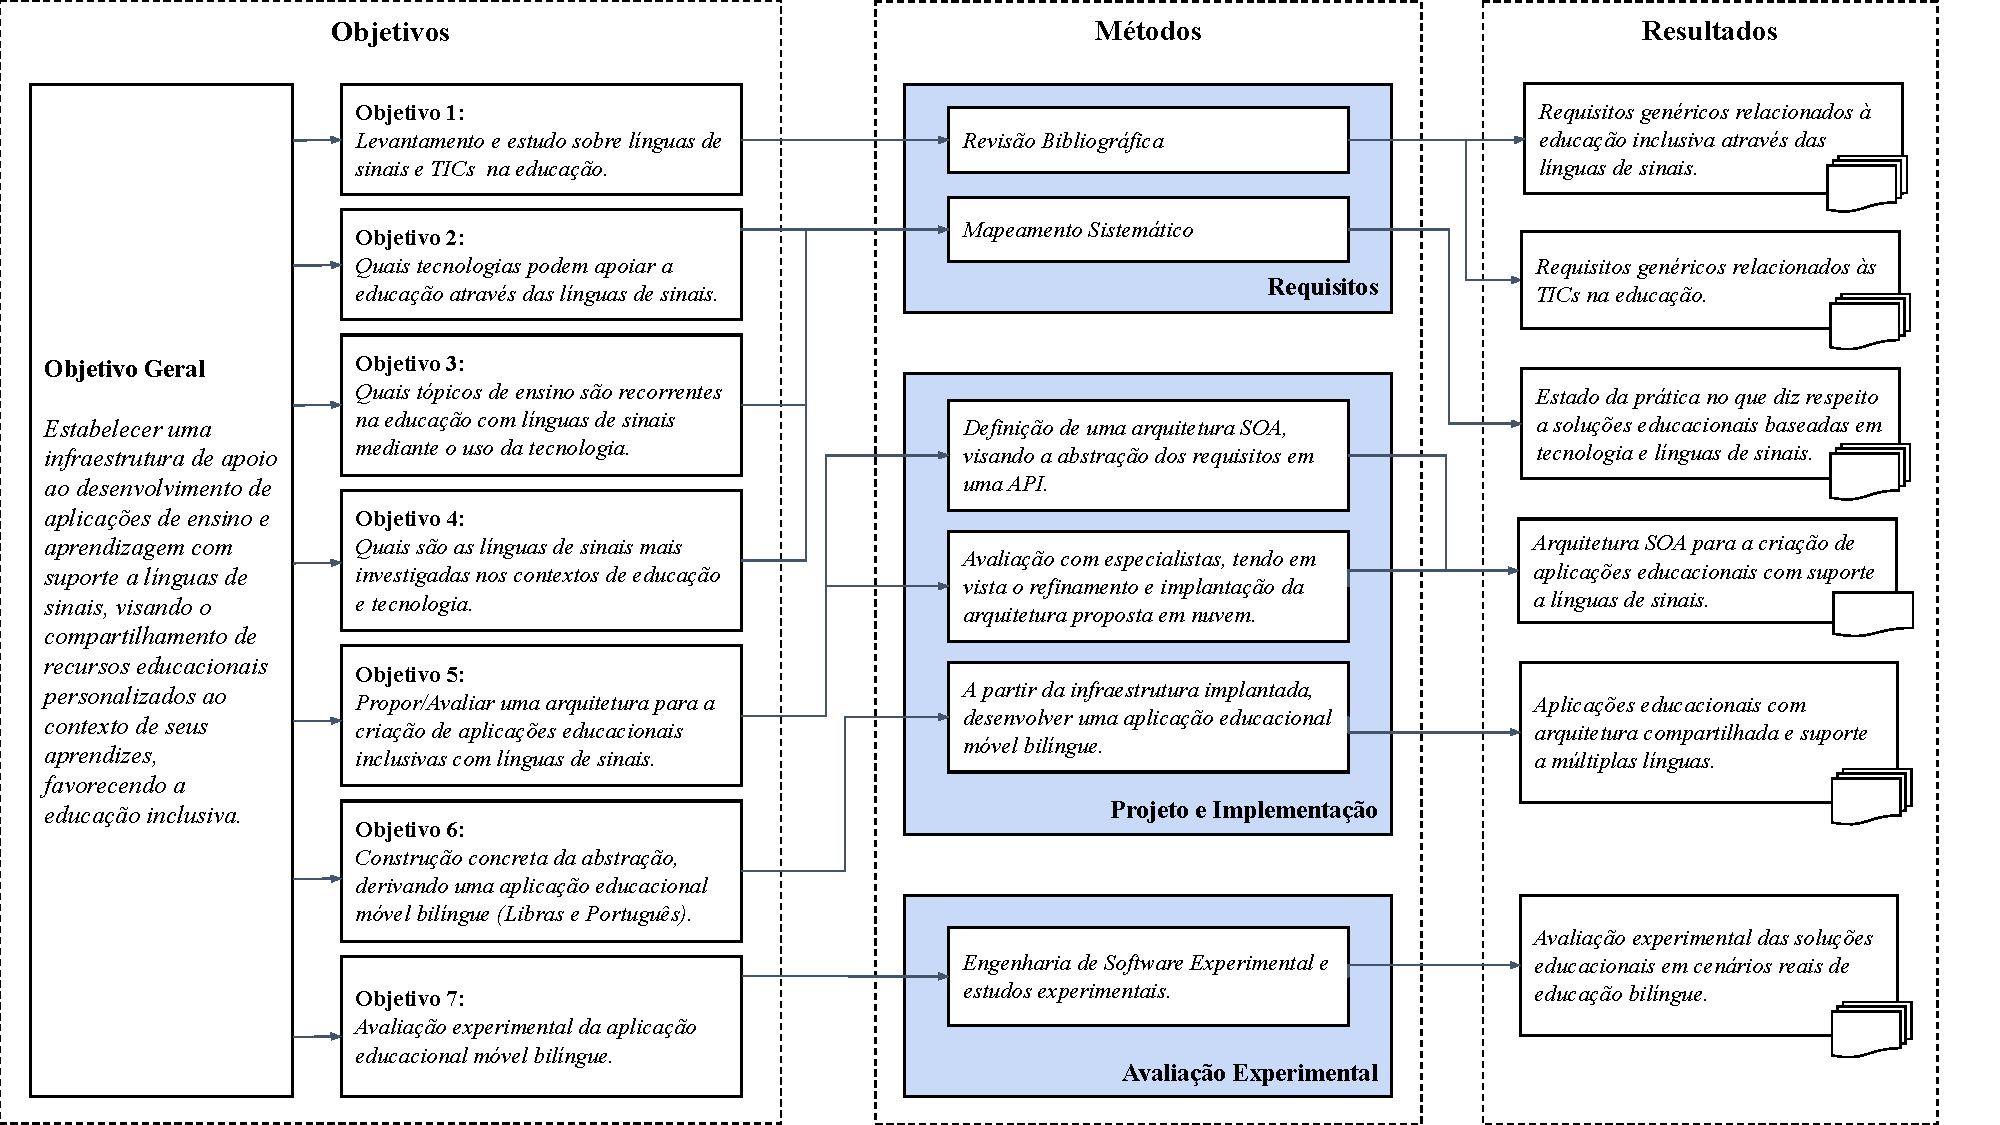
\includegraphics[width=\textwidth]{images/objectives-methods-results.pdf}}
\fautor
\end{sidewaysfigure}

\section{Publicações}

Nesta seção são apresentadas as publicações realizadas no decorrer dos quatro primeiros semestres do doutorando. Algumas delas estão relacionadas a pesquisas conduzidas em seu mestrado. Entretanto, tais publicações são importantes pois têm relação com as temáticas de ensino e aprendizagem, as quais serão exploradas diretamente neste projeto de doutorado.

\begin{itemize}

\item \uppercase{FalvoJr, V.; Martins Falvo, C.; Scatalon, L. P.; and Barbosa, E. F.} \textit{Tecnologia, Educação e Línguas de Sinais: Um Mapeamento Sistemático}. Revista Novas Tecnologias na Educação (RENOTE), 2020 -- \textit{artigo aceito em 09 de Dezembro de 2020}.

\item \uppercase{FalvoJr, V.; Martins Falvo, C.; Scatalon, L. P.; and Barbosa, E. F.} \textit{Tecnologias Aplicadas ao Ensino e Aprendizagem de Libras: Um Mapeamento Sistemático}. Anais do Simpósio Brasileiro de Informática na Educação (SBIE 2020), Natal, RN, 2020 -- \textit{artigo apresentado remotamente pelo autor principal}.

\item \uppercase{FalvoJr, V.; Scatalon, L. P.; and Barbosa, E. F.} \textit{The Role of Technology to Teaching and Learning Sign Languages: A Systematic Mapping}. Proceedings of the 50th Annual Frontiers in Education Conference (FIE 2020), Uppsala, Suécia, 2020 -- \textit{artigo apresentado remotamente pelo autor principal}.

\item \uppercase{FalvoJr, V.; Marcolino, A. S.; Duarte Filho, N. F.; OliveiraJr, E. A.; Barbosa, E. F.} \textit{Variability-based improvement of m-learning applications development}. Journal of Universal Computer Science (J.UCS) -- \textit{artigo em processo de avaliação, submetido em 04 de Fevereiro de 2020}.

\item \uppercase{Oliveira, R.; FalvoJr, V.; Barbosa, E. F.} \textit{Internet das Coisas aplicada à Educação: Um Mapeamento Sistemático}. Anais do Simpósio Brasileiro de Informática na Educação (SBIE 2019), Brasília, DF, 2019 -- \textit{artigo apresentado presencialmente pelo autor principal}.

\end{itemize}

% ---
% Finaliza a parte no bookmark do PDF, para que se inicie o bookmark na raiz
% ---
\bookmarksetup{startatroot}% 
% ---

% ----------------------------------------------------------
% ELEMENTOS PÓS-TEXTUAIS
% ----------------------------------------------------------
\postextual

% ----------------------------------------------------------
% Referências bibliográficas
% ----------------------------------------------------------
\bibliography{references}

% ---------------------------------------------------------------------
% GLOSSÁRIO
% ---------------------------------------------------------------------

%[FalvoJr] Glossário omitido

% Arquivo que contém as definições que vão aparecer no glossário
%% ---
% Glossário
% ---

% Comando para incluir todas as definições do arquivo glossario.tex
%\glsaddall
% Impressão do glossário
\printglossaries

% ----------------------------------------------------------
% Apêndices
% ----------------------------------------------------------

% ---
% Inicia os apêndices
% ---
\begin{apendicesenv}

\chapter{Síntese dos estudos primários discutidos}
\label{apendice:estudos-primarios}

\begin{small}
\setlength\tabcolsep{0.1cm}
\begin{longtable}{|c|>{\centering\arraybackslash}p{2.75cm}|c|p{10cm}|}
\hline
\textbf{Estudo} & \textbf{Tipo de Solução} & \textbf{Avatar} & \textbf{Síntese} \\ \hline
%\textit{BRA2} & Mobile & Não & Jogo baseado em mensagens instantâneas, chamado \textit{LibrasZap}. \\ \hline
\textit{BRA6} & Mobile & Sim & Avaliação das soluções \textit{Hand Talk}, \textit{ProDeaf} e \textit{Rybená}, com foco na acessibilidade linguística para crianças surdas. \\ \hline
\textit{BRA7} & Mobile & Sim & Avaliação dos aplicativos \textit{Hand Talk} e \textit{ProDeaf}, com base na teoria da aprendizagem multimídia e em heurísticas de usabilidade. \\ \hline
\textit{BRA8} & Mobile & Sim & Avaliação dos aplicativos \textit{Hand Talk} e \textit{ProDeaf}, considerando os desafios relacionados à desambiguação. \\ \hline
\textit{BRA10} & Mobile & Sim & Avaliação dos aplicativos \textit{Hand Talk} e \textit{ProDeaf}, ponderando a incidência de traduções baseadas em datilografia. \\ \hline
\textit{BRA11} & Mobile & Sim & Avaliação dos aplicativos \textit{Hand Talk} e \textit{ProDeaf}, sob a perspectiva de surdos e ouvintes no curso de formação continuada de professores. \\ \hline
\textit{BRA12} & Web & Não & Plataforma educacional intitulada \textit{SalaBil}, com ênfase na educação bilíngue (Português e LIBRAS). \\ \hline
\textit{BRA16} & Mobile & Sim & Avaliação dos aplicativos \textit{Hand Talk} e \textit{ProDeaf}, considerando a análise de tradução automática Português-LIBRAS no contexto do edital do ENEM. \\ \hline
\textit{BRA18} & Mobile & Sim & Avaliação dos aplicativos \textit{Hand Talk} e \textit{ProDeaf}, sob três perspectivas: multimidiática; multimodalidade; e quanto à socialização do sujeito surdo. \\ \hline
\textit{BRA22} & Framework & Não & \textit{Framework CAP 1.0}, que visa a criação e uso de arquiteturas pedagógicas. \\ \hline
\textit{BRA23} & Desktop & Não & Jogo idealizado para instigar o pensamento lógico de crianças surdas através de noções iniciais de robótica, denominado \textit{LibrasBot}. \\ \hline
%\textit{BRA24} & Desktop & Não & A \textit{ForcaBRAS} é uma proposta de jogo para o ensino lúdico e intuitivo da representação do alfabeto e números usando LIBRAS. \\ \hline
%\textit{BRA25} & RA & Não & Jogo da memória baseado em RA que visa apoiar usuários da LIBRAS no processo de aprendizagem. \\ \hline
%\textit{BRA27} & Framework & Não & Apresentação da \textit{CAP-APL}, uma plataforma Web que disponibiliza recursos digitais através de APs (Português e LIBRAS). \\ \hline
%\textit{BRA29} & RV & Sim & Dicionário temático visual-gestual baseado em RV para LIBRAS. \\ \hline
\textit{BRA31} & RA/RV & Não & O jogo \textit{LibrAR} utiliza RA e RV para auxiliar no ensino do alfabeto e de algarismos numéricos em LIBRAS. \\ \hline
%\textit{BRA33} & Mobile & Sim & Apresentação do aplicativo \textit{MIDOAA}, que embarca objetos de aprendizagem acessíveis para computação. \\ \hline
%\textit{BRA34} & Mobile & Não & Jogo didático multidisciplinar para alunos surdos da Educação de Jovens e Adultos, chamado \textit{Quiz ClassRoom LIBRAS}. \\ \hline
%\textit{BRA35} & Framework & Não & Plataforma \textit{Construtor de Arquiteturas Pedagógicas (CAP)} para a aprendizagem de LIBRAS. \\ \hline
%\textit{BRA36} & Mobile & Não & Aplicativo educacional móvel baseado em técnicas de gamificação que tem o objetivo de apoiar o ensino-aprendizagem da LIBRAS. \\ \hline
%\textit{BRA37} & Proposta de Design & Não & Modelo para educação inclusiva baseado na semiótica peirceana. \\ \hline
\textit{BRA39} & Web & Não & Jogo \textit{Gestus}, que tem por objetivo apresentar a Libras à crianças ouvintes, com idades entre 7 a 10 anos, de forma lúdica e humanizada. \\ \hline
%\textit{INT17} & Tradução de Máquina & Sim & Processamento de legendas para geração automática de linguagem de sinais. \\ \hline
%\textit{INT34} & RV & Sim & Ambiente de RV com suporte a chats para deficientes auditivos e para o ensino de LIBRAS. \\ \hline
\textit{INT47} & Tradução de Máquina & Sim & Solução baseada em tradução de máquina com suporte a avatares 3D, além de apresentar formalmente a concepção de um corpus com suporte a LIBRAS. \\ \hline
\textit{INT53} & Desktop & Não & Solução embarcada em DVD para o ensino da Língua de Sinais Australiana (Auslan) com possibilidade de configurações regionais. \\ \hline
\textit{INT56} & API & Não & Apresenta a arquitetura BDC-API, que traduz o material didático digital de MOOCs para surdos e cegos. \\ \hline
\textit{INT73} & Web & Não & \textit{SignQuiz}, uma aplicação educacional Web para ensino da Língua de Sinais Indiana (ISL) através de uma técnica de reconhecimento automático de sinais. \\ \hline
\textit{INT79} & Proposta de Design & Não & Proposta inicial de trabalho e metodologia que discorre sobre a criação de uma língua de sinais unificada, visando reduzir as barreiras sociais enfrentadas pelos surdos atualmente. \\ \hline
%\textit{INT80} & Proposta de Design & Sim & Desenvolvimento de um avatar intérprete de LIBRAS. \\ \hline
%\textit{INT92} & Mobile & Não & Jogo de adivinhação multiplayer para aprendizagem e prática da LIBRAS. \\ \hline
\textit{INT86} & Legendas com Línguas de Sinais & Sim & Criação de legendas automáticas em línguas de sinais para recursos educacionais online, com o objetivo de torná-los acessíveis à comunidade de deficientes auditivos. \\ \hline
\textit{INT88} & Óculos Inteligentes & Não & Uso do conceito de RA através de óculos inteligentes no apoio a pessoas com deficiência auditiva. \\ \hline
\textit{INT109} & Desktop & Não & Jogo educacional para o aprendizado de operações matemáticas e números em LIBRAS, denominado \textit{MatLIBRAS Racing}. \\ \hline
\end{longtable}
\end{small}


\end{apendicesenv}
% ---


% ----------------------------------------------------------
% Anexos
% ----------------------------------------------------------

% ---
% Inicia os anexos
% ---
%[FalvoJr] Anexos omitidos
%\begin{anexosenv}
%
%    \chapter{Páginas interessantes na Internet} 
%    \label{chapter:paginas-interessantes}
%    \input{tex/annex/paginas-interessantes}
%
%\end{anexosenv}
% ---

\end{document}